\documentclass[12pt, a4paper, twoside]{book}


%------------------------
% IMPORT PACKAGES
%-----------------------
\usepackage[english ]{babel}
\usepackage[utf8x]{inputenc}
\usepackage{amsmath,amsthm}
\usepackage{amsfonts}
\usepackage{graphicx}
\usepackage{adjustbox}
\usepackage{float,subfloat}
\usepackage{wrapfig}
\usepackage{lipsum}
\usepackage{bbm}
\usepackage{bm}
\usepackage{empheq}
\usepackage{mathtools}
\usepackage{algorithm,algpseudocode}
\usepackage{booktabs,longtable}
\usepackage{array}
\usepackage{hyperref}
\usepackage{siunitx}
\sisetup{output-exponent-marker=\ensuremath{\mathrm{e}}}
\usepackage[acronym,toc,nohypertypes={acronym,notation},nonumberlist,automake]{glossaries}
\usepackage{fancyhdr}
\usepackage[algo2e]{algorithm2e}

%\usepackage{appendix}

%\DeclareMathOperator*{\sup}{sup}
\DeclareMathOperator*{\argmax}{arg\,max} % argmax operator

%% remark theoremstyle
%\newtheoremstyle{break}
%{\topsep}{\topsep}%
%{\itshape}{}%
%{\bfseries}{}%
%{\newline}{}%
%\theoremstyle{break}
%\newtheorem{remark}{Remark}[section]

% problem theoremstyle
\newtheoremstyle{problemstyle}  % <name>
{10pt}  % <space above>
{10pt}  % <space below>
{\normalfont} % <body font>
{}  % <indent amount}
{\bfseries\itshape} % <theorem head font>
{\normalfont\bfseries:} % <punctuation after theorem head>
{.5em} % <space after theorem head>
{} % <theorem head spec (can be left empty, meaning `normal')>
\theoremstyle{problemstyle}
\newtheorem{problem}{Problem}[section] % Comment out [section] toremove section number dependence
\newtheorem{definition}{Definition}[section]
\newtheorem{theorem}{Theorem}[section]
\newtheorem{proposition}{Proposition}[section]
\newtheorem{remark}{Remark}[section]
\newtheorem{lemma}{Lemma}[section]
% create command for variance in math mode
\newcommand{\Var}[1]{\operatorname{Var}\left[#1\right]}


\makeglossaries



\newacronym{GH}{GH}{Generalized Hyperbolic}
\newacronym{ED}{ED}{Event-Driven}
\newacronym{TD}{TD}{Time-driven}
\newacronym{ATM}{ATM}{Air Traffic Management}
\newacronym{DES}{DES}{Discrete Event System}
\newacronym{ODAA}{ODAA}{Optimal Dynamic Asset Allocation}
\newacronym{GBM}{GBM}{Geometric Brownian Motion}
\newacronym{SDE}{SDE}{Stochastic Differential Equations}
\newacronym{CPPI}{CPPI}{Constant-Proportion Portfolio Insurance}
\newacronym{MPT}{MPT}{Modern Portfolio Theory}
\newacronym{CAPM}{CAPM}{Capital Asset Pricing Model}
\newacronym{EMH}{EMH}{Efficient-Market Hypotesis}
\newacronym{BS}{BS}{Black and Scholes}
\newacronym{G}{G}{Gaussian}
\newacronym{GM}{GM}{Gaussian Mixture}

% define environment ABSTRACT
\newenvironment {abstract}%
{\cleardoublepage \null \vfill \begin{center}%
	\bfseries \abstractname \end{center}}%
{\vfill \null }
% define envirnoment SOMMARIO
\newenvironment {sommario}%
{\cleardoublepage \null \vfill \begin{center}%
		\bfseries \abstractname \end{center}}%
{\vfill \null }
\begin{document}


%----------------------------------------------------------------------------------------
% COVER PAGE
%----------------------------------------------------------------------------------------
\pagestyle{empty}
\begin{titlepage}

	\begin{center}
		\normalsize 
			\textsc{Politecnico di Milano}\\
			Scuola di Ingegneria Industriale e dell'Informazione\\
      		Corso di Laurea Magistrale in Ingegneria Matematica\\
	\end{center}
	\vspace{.6cm}
	
	\begin{figure}[htpb]
		\centering
		
\includegraphics[width=4cm]{Cover/polimi}
	\end{figure}
	\vspace{.6cm}
	
	\begin{center}
		\LARGE
			\textsc{A Stochastic Reachability Approach to Asset Allocation}
	\end{center}
	\vspace{1.6cm}

	\begin{flushleft}
		\large
		\begin{tabular}{ll}
		Relatore:    & Prof. Emilio BARUCCI      \\
		Correlatore: & Dott. Gianni POLA
		\end{tabular}
		\vspace{1cm}
	\end{flushleft}
	
	\begin{flushright}
		\large
		Tesi di Laurea di:\\
		Andrea SCHIAVON\\
		Matr. 852559\\		
	\end{flushright}
	
	\vspace*{\fill}
	\begin{center}
		Anno Accademico 2016-2017
	\end{center}
	
\end{titlepage}


%----------------------------------------------------------------------------------------
% ABSTRACT
%---------------------------------------------------------------------------------------

%% Set page numbers of the introduction to roman  
\frontmatter
\pagestyle{plain}

\begin{abstract}
	Before the 1950s, managing other people's money was a discipline as far away from being scientifically dictated as it could ever get. For instance, before Markowitz's revolutionary paper \textit{Portfolio Selection}, diversification was not a universally recognized practice in Asset Allocation. Markowitz's work paved the way for new ideas from different scientific and academical fields to influence Finance and Asset Allocation in particular.
	
	Continuing along this line, in this thesis cutting-edge results in Stochastic Reachability (which is a concept belonging to the theory of Control Systems) are employed to tackle the Asset Allocation problem. In particular, once an investor has specified his risk profile (through a value-at-risk specification) and a target return, the model will output an optimal investment strategy having the feature of maximizing the probability of reaching the target return while keeping the risk under control. This strategy will exhibit a \textit{contrarian} behavior, namely it prescribes to buy risky assets (in order to achieve a riskier position) when performance is down and to sell them when performance is up.
	
	
	What are the drivers that lead a portfolio manager to rebalance portfolio weights? In Part I, the case where time triggers a portfolio rebalancing will be explored. Although this Time-Driven approach is the most intuitive, it might incur in non-negligible transaction costs if the rebalancing frequency is high. On the other hand, in Part II, what causes the portfolio mix to be readjusted will be the fact that the risky asset cumulative return hits a lower or upper barrier. This portfolio rebalancing mechanics leads to the so-called Event-Driven approach to Asset Allocation.
	
	\vspace{0.5cm}
	\noindent
	\textbf{Keywords}: Asset Allocation, Stochastic Reachability, Time-Driven approach, Event-Driven approach.

\end{abstract}



\begin{otherlanguage}{italian}
	\begin{abstract}
		Contrariamente a quanto accade oggi per i maggiori investitori istituzionali, prima degli anni '50 chi investiva in borsa lo faceva senza adottare un metodo rigorosamente scientifico. Il cambio di rotta avvenne nel 1952, quando Harry Markowitz, fondatore della moderna teoria del portafoglio, pubblicò \textit{Portfolio Selection}, un articolo che aprì la strada ad un flusso di nuove idee provenienti dall'accademia e da svariate discipline scientifiche, idee che saranno destinate a rivoluzionare il modo di investire nei decenni successivi. 
		
		Proseguendo in questa direzione, nel nostro lavoro vengono utilizzati recenti risultati in Stochastic Reachability (concetto sviluppato nella teoria dei Sistemi di Controllo) per riadattarli in un contesto di Asset Allocation. In particolare, una volta individuato un adeguato profilo di rischio (tramite un'indicazione di value-at-risk) e un rendimento da raggiungere, il modello produrrà una strategia di investimento che massimizza la probabilità di raggiungere tale rendimento tenendo allo stesso tempo sotto controllo il rischio. Questa strategia avrà la caratteristica di essere \textit{Contrarian}, cioè prescrive di acquistare titoli rischiosi quando la performance del portafoglio è buona mentre prescriverà di venderli, in favore di titoli privi di rischio, se la performance è bassa.
		
		Con che criterio dunque, un gestore decide di ribilanciare i pesi di portafoglio? Nella prima parte del lavoro verrà presentato l'approccio Time-Driven, in cui è il tempo a dettare la riallocazione dei pesi (e.g. settimanalmente). Nonostante questo sia il metodo più intuitivo, ha come svantaggio gli elevati costi di transazione nel caso di frequenza di riallocazione alta. Nella seconda parte invece, l'approccio che si segue è quello Event-Driven. Ciò significa che una riallocazione di portafoglio viene effettuata solo quando il valore assoluto del rendimento cumulato dell'asset rischioso supera una certa soglia.
		
		
		\vspace{0.5cm}
		\noindent
		\textbf{Parole chiave}: Asset Allocation, Stochastic Reachability, Time-Driven approach, Event-Driven approach.
		
		
	\end{abstract}
\end{otherlanguage}



%----------------------------------------------------------------------------------------
%	LIST OF CONTENTS/FIGURES/TABLES PAGES
%----------------------------------------------------------------------------------------

\tableofcontents
\listoftables
\addcontentsline{toc}{chapter}{List of Tables}
\listoffigures
\addcontentsline{toc}{chapter}{List of Figures}
\listofalgorithms
\addcontentsline{toc}{chapter}{List of Algorithms}
\printglossaries


%----------------------------------------------------------------------------------------
%	THESIS CONTENT - CHAPTERS
%----------------------------------------------------------------------------------------

\mainmatter

\begin{frame}{Che cos'è l'Asset Allocation?}
	
    \begin{definition}
			L’\textbf{asset allocation} è il processo con il quale si decide in che modo distribuire le risorse fra diversi i possibili investimenti
    \end{definition}
	\begin{figure}
		\centering
		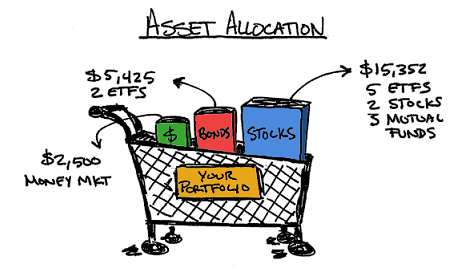
\includegraphics[width=.6\linewidth]{Images/AA}
	\end{figure}
\end{frame}


\begin{frame}{Raggiungibilità Stocastica: un esempio di applicazione}
	\begin{block}{Gestione del Traffico Aereo}
		\begin{figure}
			\centering
			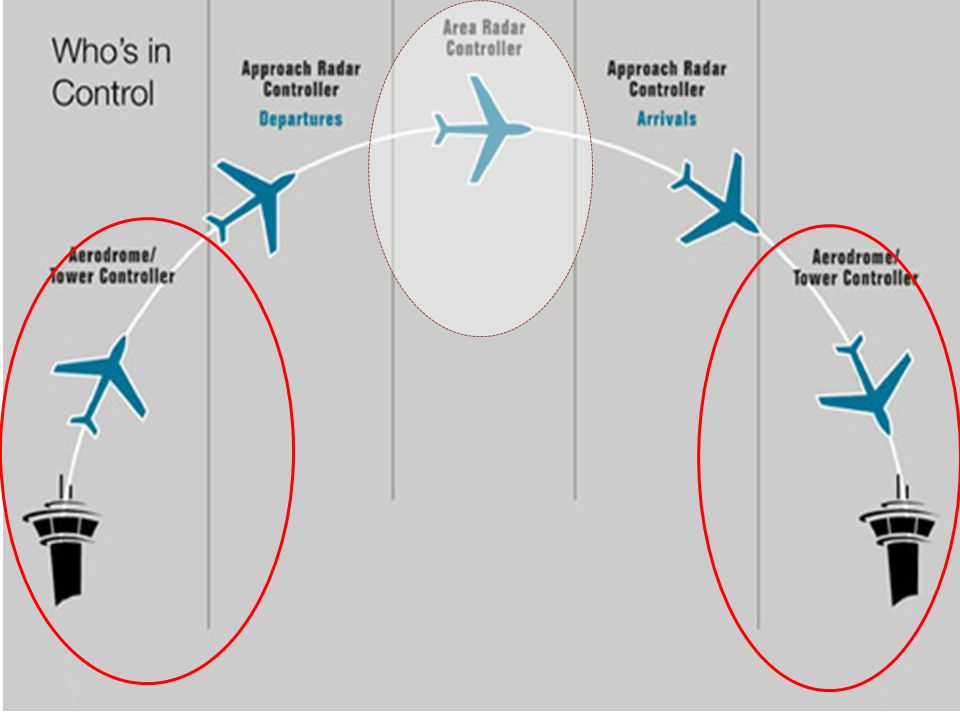
\includegraphics[width=0.7\linewidth]{Images/ATM}
		\end{figure}
	\end{block}
\end{frame}
\begin{frame}{Raggiungibilità Stocastica in Finanza}
	
		\begin{figure}
			\centering
			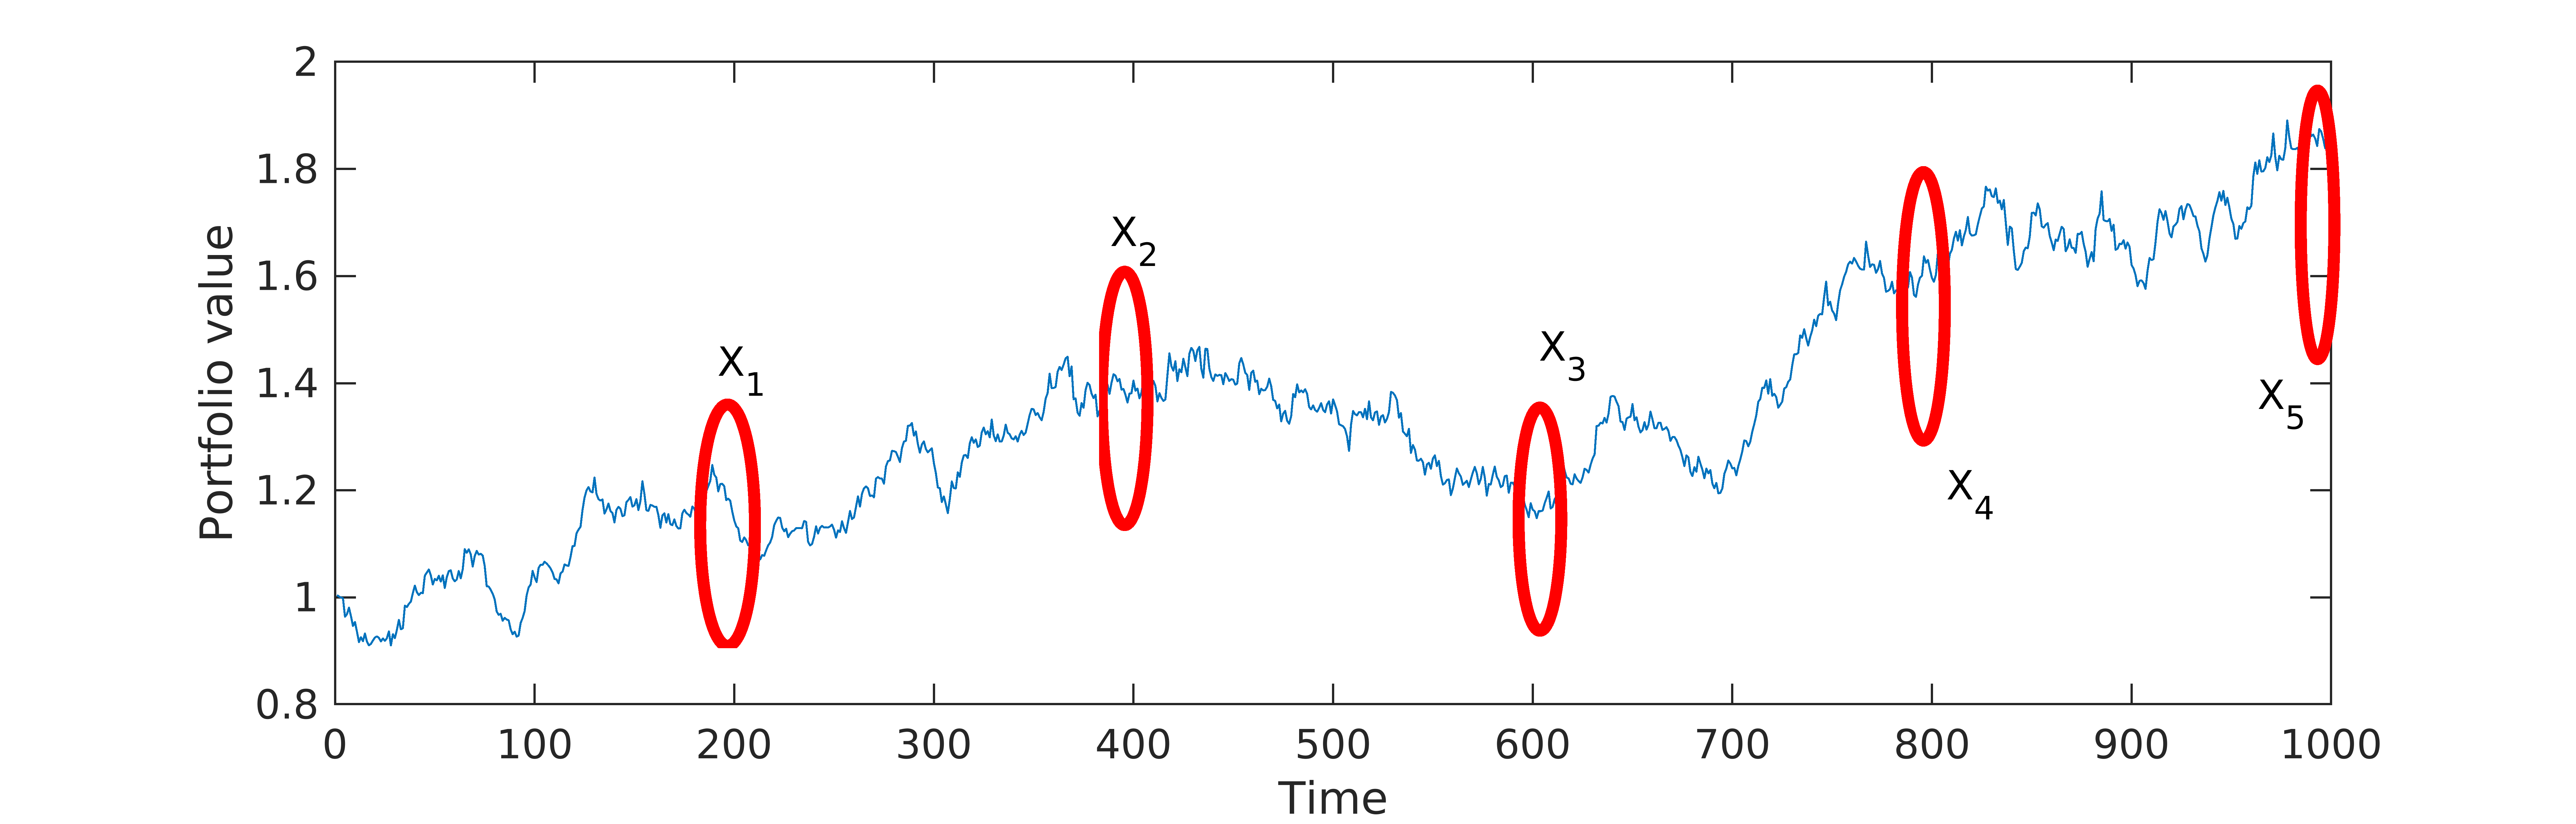
\includegraphics[width=1.1\linewidth]{Images/Reachability}
		\end{figure}

\end{frame}





\part{Time-driven approach}\label{part:1}

\chapter{Model Description}\label{chpt:Model_Description}
\glsresetall
In this chapter, first the basic financial quantities are introduced and the asset allocation problem is stated, then the same problem will be embedded in a dynamical control system framework which will allows us to develop the stochastic reachability approach to portfolio construction. We closely follow \cite{Pola12},\cite{Pola06} and \cite{Pola}.
\section{Portfolio construction}
In the financial industry, a group of securities that exhibits similar characteristics in the market place and is subject to the same regulation is called \textbf{asset class}. Typical asset classes include stocks, bonds, real estate, cash and commodities. The discipline consisting in allocating investor's wealth among different asset classes is called \textbf{asset allocation}. We will now introduce the financial quantities and a formal mathematical setting suitable for describing the asset allocation problem. Let $(\Omega,\mathcal{F},\mathbb{P})$ be the underlying  probability space and consider a discrete set of time indexed by $k \in \mathbb{N}$. Moreover, let us consider a universe of $m \in \mathbb{N}$ asset classes. Asset classes' performance at period $k$ is described by a $m$-dimensional random vector 
$\bm{w}_k = \begin{bmatrix} w_k(1),\ldots,w_k(m)\end{bmatrix}^T $ 
where 
$$ w_k(i) = \frac{z_k(i)-z_{k-1}(i)}{z_{k-1}(i)}, \quad i = 1,\ldots,m$$
is the rate of return of the $i$-th asset class and $\{z_k(i)\}_{k \in \mathbb{N}}$ the $i$-th asset class price process. In general, the correlation of $\bm{w}_k$ can be of two kinds:
\begin{itemize}
	\item \textit{synchronous} correlation, that is the correlation among different asset class at the same time period (i.e. correlation between $w_k(i)$ and $w_k(j)$ for $i,j=1,\ldots,m$)
	\item \textit{time-lagged} correlation, that is the correlation among different asset class at different time period (i.e. correlation between $w_k(i)$ and $w_{k'}(j)$, with $k\neq k'$ for $i,j=1,\ldots,m$).
\end{itemize}
As the time-lagged correlation is usually negligible for short time period, $\bm{w}_k$ is a synchronous-correlated random vector. Standard notation is used for Expected Returns and Covariance Matrix 

\begin{align*}
\mu_k(i) & = \mathbb{E}\big[w_k(i)\big], \quad i = 1,\ldots,m \quad k \in \mathbb{N} \\[1.5ex]
\Sigma_k(i,j) &  = \mathbb{E}\bigg[\Big(w_k(i)-\mu_k(i)\Big)\Big(w_k(j)-\mu_k(j)\Big)\bigg], \quad i,j = 1,\ldots,m \quad k \in \mathbb{N}.
\end{align*}

 An asset allocation at period $k \in \mathbb{N}$ is a vector $\bm{u}_k \in \mathbb{R}^m$ whose $i$-th element indicates the percentage of wealth to be invested in asset class $i$. This vector is the leverage the asset manager has at his disposal for driving the portfolio value towards his goals. The portfolio performance over the period $[k-1,k]$ is measured by the portfolio return $$r_{k+1}=\frac{x_{k+1}-x_{k}}{x_k}$$ where $\{x_k\}_{k \in \mathbb{N}}$ is the portfolio value process. The portfolio return can also be expressed as a weighted average of each asset class return  as $$ r_{k+1} = \bm{u}_k^T \bm{w}_{k+1}.$$
 By combining the two previous relations we get the following recursive equation 
 \begin{equation}
 \boxed{x_{k+1} = x_k (1 + \bm{u}_k^T \bm{w}_{k+1})}
 \end{equation}
 which describes the time evolution of portfolio value. In plain words, the \textbf{asset allocation problem} consists in choosing the vector $\bm{u}_k$ at each time period $k \in \mathbb{N}$ (called \textbf{rebalancing time}) so as to achieve the  investor's goal. If the investor is mainly concerned about the final return, the allocation strategy is called \textbf{total-return allocation}. On the other hand, if his objective is beating a benchmark (index created to include multiple securities representing some aspect of the total market), the strategy is called \textbf{benchmark allocation}. In the following, we will consider only total-return portfolios.
 
 As well as setting the target return, the investor specifies other requirements that the portfolio manager must take into consideration. This means that  the asset allocation vector $\bm{u}_k$ is bound to stay within a feasible set $U_k$, for each $k \in \mathbb{N}$. In this work, the feasible set $U_k$ is obtained by imposing the following set of constraints
 \begin{itemize}
 	\item \textit{budget} constraint: $\sum_{i=1}^{m}u_k(i)=1$, all the wealth is invested in the portfolio
 	\item \textit{long-only} constraint: $u_k(i) \geq 0,\quad i = 1,\ldots,m$, no short-selling is allowed
 	\item \textit{risk} constraint: the metric value-at-risk ($V@R$) is used to limit portfolio risk. 
 \end{itemize}
The form of the \textit{risk} constraint will actually depend on the model used to describe the probabilistic properties of vector $\bm{w}_k$. In Chapter \ref{chpt:assetclass_returns} we will tackle this issue.
\section{Stochastic Reachability Approach}
In the previous section the financial setting has been laid, now it will be embedded in a more general framework by employing the theory of dynamical systems. We will see that this formalism will allow us to formulate the asset allocation problem as a \textbf{stochastic reachability} problem which will be solved by using \textbf{dynamic programming} (DP) techniques.
\subsection{The concept of Stochastic Reachability}
"In general terms, a reachability problem consists of determining if a given system trajectory will eventually enter a prespecified set starting from some initial state" \cite{Boj2012}. For deterministic systems, reachability analysis amounts to compute the set of states that can be reached by system trajectories. However, most of real-life problem are non-deterministic and uncertainty must be taken into account. In these cases, the main concern is determining the probability that the system reaches a prespecified set. "Typically, a certain part of the state space is "unsafe" and the control input of the system has to be chosen so as to keep the state away from it" \cite{Boj2012}. One of the most successful application of stochastic reachability techniques has been \gls{ATM}. "Within the \gls{ATM} context, safety-critical situation arise during flight when an aircraft comes closer than a minimum allowed distance to another aircraft or enters a forbidden region of the airspace. In the current \gls{ATM} system, air traffic controllers are in charge of guaranteeing safety by issuing to pilots corrective actions on their flight plans when a safety-critical situation is predicted" \cite{Boj2012}.

Conversely, when Stochastic Reachability is applied to the financial asset allocation problem, a dual viewpoint is taken. In this context, the focus is on driving the system state (the value of a portfolio of securities) into a "safe" set, and computing the probability that this occurs. The air traffic controller becomes a portfolio manager and signals issued to the pilot turns into orders to traders to buy or sell assets so as to adjust the portfolio mix.
\subsection{Mathematical Formulation}
 Let us introduce the following stochastic discrete-time dynamic control system
\begin{equation}
\label{eq:state_equation}
x_{k+1} = f(x_k,\bm{u}_k,\bm{w}_{k+1}) = x_k (1 + \bm{u}_k^T \bm{w}_{k+1}) 
\end{equation}
where, for any $k \in \mathbb{N}$
\begin{itemize}
	\item $x_k \in \mathcal{X} = \mathbb{R}$ is the system state, $\mathcal{X}$ the system space
	\item $\bm{u}_k \in U \subset \mathbb{R}^m$ is the control input, $U$ the control input space
	\item $\bm{w}_{k}$ is a $m$-dimensional random vector with density function $p_{\bm{w}_k}$
\end{itemize}

Let $\mathcal{U} = \big\{ \mu : \mathcal{X} \times \mathbb{N} \rightarrow U \big\}$ be the class of controls we focus on. Any $\mu \in \mathcal{U}$ is a map such that for any $x \in \mathcal{X}$ and any $k \in \mathbb{N}$, it associates an asset allocation vector $\bm{u}_k \in U$.
Given $N \in \mathbb{N}$ we define the set of control sequences as \[\mathcal{U}_N = \Big\{\pi = \{\mu_k\}_{k=0,\ldots,N}  : \mu_k \in \mathcal{U} \Big\}\] and call any $\pi \in \mathcal{U}_N$ a \textbf{control policy}. Moreover, let us denote by $\pi^k$ a control policy starting at period $k$, that is $\pi^k=\{\mu_k,\ldots,\mu_N\}$. We have all the ingredients to formulate the asset allocation problem in stochastic reachability terms.
\begin{problem}[Optimal Dynamic Asset Allocation]\label{prb:ODAA}
Given a finite time horizon $N \in \mathbb{N}$ and a sequence of target sets $\{X_1,\ldots,X_N \} $ such that each target set is a subset of the state space $\mathcal{X}$, find the optimal control policy $\pi^{\star} \in \mathcal{U}_{N-1}$ that maximizes the following objective function 
\begin{equation}\label{eq:obj_fun_ODAA}
\mathbb{P}\Big(\big\{\omega \in \Omega : x_0 \in X_0,\ldots,x_N \in X_N \big\} \Big).
\end{equation}
\end{problem}
The target sets $\{X_1,\ldots,X_N \}$ represent the investor's goal and we can think of them as the "good" states where we want the portfolio value to belongs to. For instance, a target set could be $X_k = [\underline{x}_k,\infty)$. Problem (\ref{prb:ODAA}) is going to be solved by resorting to dynamic programming. However, before doing that, we need to make explicit the dependence of (\ref{eq:obj_fun_ODAA}) on the control policy $\pi$. To this end, let $p_{f(x,\bm{u},\bm{w}_{k+1})}$ be the density of random variable (\ref{eq:state_equation}) and let us introduce the following function.
\begin{definition}[Value function]
	Given a sequence of target sets $\{X_k\}_{k\geq0}$, the \textbf{value function} associated with Problem \ref{prb:ODAA} is the following real map
	\begin{align*}
	V \colon \mathbb{N}\times \mathcal{X}\times \mathcal{U} & \rightarrow [0,1]\\
	(k,x,\pi^k) & \mapsto V(k,x,\pi^k)
	\end{align*}
	such that 
	\[V(k,x,\pi^k)=
	\begin{cases}
	    \mathbbm{1}_{X_N}(x) & \quad \text{if} \quad k = N \\
	    \int_{X_{k+1}}V(k+1,z,\pi^{k+1})p_{f(x,\bm{u},\bm{w}_{k+1})}(z)\mathrm{d}z & \quad \text{if} \quad k = N-1,\ldots,0.
	\end{cases}
	\]
	\end{definition}
It is now possible to link the objective function (\ref{eq:obj_fun_ODAA}) to the value function in the following way (see \cite{Pola}) \[\mathbb{P}\big(\{\omega \in \Omega : x_0 \in X_0,\ldots,x_N \in X_N \} \big) = V(0,x_0,\pi). \]
This result is extremely important since it allows us to rewrite the ODAA problem in terms of the value function as follows
\begin{problem}[Optimal Dynamic Asset Allocation 2]\label{prb:ODAA2}
  Given a finite time horizon $N \in \mathbb{N}$ and a sequence of target sets $\{X_1,\ldots,X_N \}$, find $$\pi^{\star} = \argmax_{\pi \in \mathcal{U}_{N-1}}V(0,x_0,\pi). $$	
\end{problem}
So far, we have reached an intermediate point where the ODAA problem has been restated in terms of a value function $V$. In this way, we can directly apply dynamic programming tools and solve it. The result is given in the following theorem, that is the cornerstone on which this work is based on.
\begin{theorem}[ODAA algorithm]\label{thm:rec_algo}
	the optimal value of the \gls{ODAA} Problem \ref{prb:ODAA2} is \[p^{\star} = J_0(x_0),\] where for any $x \in \mathcal{X},$ $J_0(x)$ is the final step of the following algorithm
	\begin{empheq}[box=\fbox]{align} \label{eq:rec_algo}
	J_N(x) & = \mathbbm{1}_{X_N}(x) \nonumber \\
	J_k(x) & = \sup_{\bm{u}_k \in U_k}\int_{X_{k+1}}J_{k+1}(z)p_{f(x,\bm{u}_k,\bm{w}_{k+1})}(z)\mathrm{dz} \\
	& k = N-1,\ldots,1,0. \nonumber
	\end{empheq}
\end{theorem}
The previous result provides us with a backward procedure (it starts at time $N$ and ends at time $0$) whose outputs are the optimal control policy $\pi^{\star}=\{\mu_0^{\star},\ldots,\mu_{N-1}^{\star}\}$ and the optimal joint probability $p^{\star}$ of reaching the target sets. It is worth pointing out some interesting features of algorithm in (\ref{eq:rec_algo}):
\begin{itemize}
	\item $J_k(x)$ is a function of portfolio realization $x \in \mathcal{X}$ at time $k$. This dependence is hidden behind the probability density function $p_{f(x,\bm{u}_k,\bm{w}_{k+1})}$
	\item the constrained optimization must be numerically carried out in a space ($U_k$) of dimension $m \in \mathbb{N}$. At each iteration $k = N-1,\ldots,1,0$, the optimization has to be repeated for each $x$ belonging to a suitable discretized grid
	\item the algorithm presented in theorem (\ref{thm:rec_algo}) does not depend on the particular distribution of random variable $f(x,\bm{u}_k,\bm{w}_{k+1})$. This fact gives us enough freedom to look outside the usual Guassian world
	\item given a period $k \in \mathbb{N}$ and a portfolio value realization $x \in \mathcal{X}$, $\mu_k^{\star}(x) \in U_k$ tells us which is the optimal allocation mix of our portfolio.
\end{itemize}

We now ask ourselves which probability distributions are suitable for vector $\bm{w}_{k+1}$; the answer to this question is the main objective of the next chapter.


\chapter{Asset Class Returns modeling}\label{chpt:assetclass_returns}
	
In this chapter, we address the asset class returns modeling issue. As it was noted above, the ODAA algorithm does not depend on a particular distribution for the asset class returns vector $\bm{w}_{k+1}$. However, by looking at equation  (\ref{eq:rec_algo}) we see that we need the explicit analytical form for the density function $p_{f(x,\bm{u}_k,\bm{w}_{k+1})}$. For this reason, we will be dealing exclusively with probability distributions closed under linear combination. In this work, we propose three such distributions:
\begin{itemize}
	\item Gaussian
	\item Gaussian Mixture
	\item Generelized Hyperbolic
\end{itemize}
For each of them, first we will give a theoretical introduction, secondly derive the portfolio value density function $p_{f(x,\bm{u}_k,\bm{w}_{k+1})}$ and an expression for the risk constraint (which depends on the distribution chosen).
\section{Gaussian model}
The first probability distribution we considered is the Gaussian 
\begin{definition}[Gaussian random vector]\label{def:gauss_rv}
	A $m$-dimensional random vector $\bm{w} = [w_1,\ldots,w_m]^T$ is \textbf{Gaussian} if every linear combination $\sum_{i=0}^{m}u_iw_i = \bm{u}^T \bm{w}$ has a one-dimensional Gaussian distribution.
\end{definition}
Let the asset class returns random vector $\bm{w}_{k+1}$ follow a Gaussian distribution with mean $\bm{\mu}$ and covariance matrix $\bm{\Sigma}$  $\big(\bm{w}_{k+1} \sim \mathcal{N}(\bm{\mu},\bm{\Sigma})\big)$. By definition we have \[x(1 + \bm{u}_k^T \bm{w}_{k+1}) \sim \mathcal{N}\Big(\underbrace{x(1 + \bm{u}_k^T \bm{\mu})}_{\tilde{\mu}}, \underbrace{x^2\bm{u}_k^T \Sigma \bm{u}_k}_{\tilde{\sigma}^2}\Big)\]
hence
\begin{equation}
\boxed{p_{f(x,\bm{u}_k,\bm{w}_{k+1})}(z) =  \frac{1}{\sqrt{2\pi}\tilde{\sigma}}\exp\big\{ -\frac{1}{2}\frac{(z-\tilde{\mu})^2}{\tilde{\sigma}^2}\big\}, \quad z \in \mathbb{R}.}
\end{equation}
 

Let us now introduce the two important concepts of loss function and value-at-risk that we will use to derive the portfolio risk constraint
\begin{definition}[loss function]\label{def:loss_function}
	Denoting the value of our portfolio at time $k \in \mathbb{N}$ by $x_{k+1}$, the \textbf{loss function} of the portfolio over the period $[k,k+1]$ is given by \[ L_{k+1}:= -\frac{(x_{k+1}-x_k)}{x_k}= -r_{k+1} = -\bm{u}_k^T \bm{w}_{k+1}.  \]
\end{definition}
\begin{definition}[Value-at-risk]
	Given some confidence level $1-\alpha \in (0,1) $ the \textbf{value-at-risk} ($V@R_{1-\alpha}$) of our portfolio is \[ V@R_{1-\alpha} = \inf\{l\in \mathbb{R} : \mathbb{P}\big(L_{k+1} \leq l \big) \geq 1-\alpha \}. \]
\end{definition}
	

The V@R is a risk measure commonly use by financial institutions to asses the risk they run to carry a portfolio for a specified period of time (the portfolio must be kept constant during this time period). For instance, if our portfolio has a $V@R_{0.99} = 7\%$, this means that with a confidence level of $99\%$ our portfolio does not suffer a loss greater or equal than $7\%$ over per period $[k,k+1]$ (e.g. a month). In our case, we receive the V@R specification ($V@R_{0.99} = 7\%$) in input by the investor (it is an indicator of its risk-aversion) and we will construct an asset allocation $\bm{u}_k$ that satisfies this risk constraint at each $k \in \mathbb{N}$.

Using definition (\ref{def:gauss_rv}) we have \[ L_{k+1} \sim \mathcal{N}\big(\underbrace{-\bm{u}_k^T \bm{\mu}}_{\mu_p},\underbrace{\bm{u}_k^T \bm{\Sigma} \bm{u}_k}_{\sigma^2_p} \big)\] therefore
\begin{align*}
\mathbb{P}\big(L_{k+1} \leq V@R_{1-\alpha}\big) 
& = \mathbb{P}\Big(Z \leq \frac{V@R_{1-\alpha} - \mu_p}{\sigma_p}  \Big) \\
& = 1 - \alpha
\end{align*}
\begin{equation}\label{eq:var_const_gaussian}
\implies \boxed{V@R_{1-\alpha} \geq -\bm{u}_k^T\bm{\mu} + z_{1-\alpha} \sqrt{\bm{u}_k^T \bm{\Sigma} \bm{u}_k}}
\end{equation}
where $Z$ is a standard normal random variable and $z_{1-\alpha}$ is the $1-\alpha$ quantile of the standard normal distribution. The \textit{risk} constraint in equation (\ref{eq:var_const_gaussian}), together with the \textit{budget} and \textit{long-only} constraint, define the control space $U_k$ which is the feasible set of the constrained optimization problem given in theorem (\ref{thm:rec_algo}).
\section{Gaussian Mixture model}
In this section we present the second asset class returns model, the \textbf{Gaussian Mixture model} (GM). After introducing the GM distribution we will derive the density and the \textit{risk} constraint, as we did for the Gaussian model. We closely follow \cite{BUCKLEY2008}.

The standard assumption that asset returns have a multivariate Gaussian distribution is a reasonable first approximation to reality and it usually has the big advantage of generating analytically tractable theories (e.g. Markowitz portfolio theory). However, the Gaussian model does not capture two important key features of asset returns which are observed in the market real data:
\begin{enumerate}
	\item the skewed (asymmetric around the mean) and leptokurtic (more fat-tailed than the Gaussian) nature of marginal probability density function
	\item the asymmetric correlation between asset returns, that is the tendency of volatilities and correlations to depend on the prevailing market conditions.
\end{enumerate}
To overcome this shortcomings, the Gaussian Mixture distribution is a validate alternative to the Gaussian one. Loosely speaking, the pdf of a GM random vector id a linear combination of Gaussian pdfs (called Gaussian regimes or mixing components). This closeness to the Normal distribution offers a good trade-off between analytical tractability and parsimony in the number of parameters. By adopting a GM model, it is possible to represent protuberances on the probability iso-density contour, as can be seen in the following figure
\begin{figure}[H]
	\caption{Example of a GM density contour plot with two mixing components.}
	\centering
	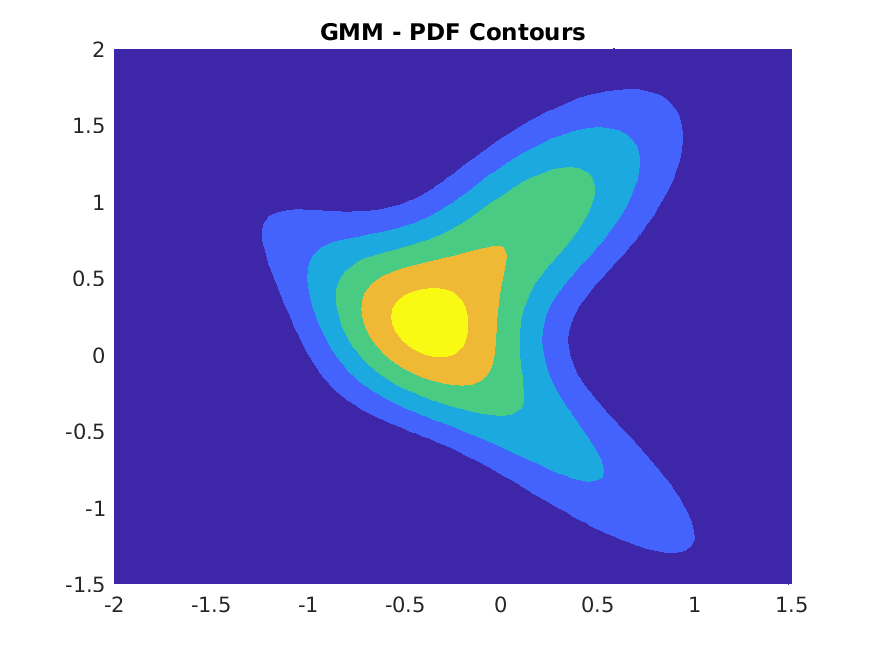
\includegraphics[width=0.7\textwidth]{Images/GMdensity.png}
\end{figure}
To obtain this highly non-linear dependence structure, we would usually need cross-moments of all order; a big advantage of the GM distribution is that its dependence structure is fully and conveniently captured by the means, covariance matrices and weights of each Gaussian regime (as we will see in the following).

We start the more formal introduction on the GM distribution giving its definition
\begin{definition}[GM distribution]
	An $m$-dimensional random vector $\bm{Z}$ has a \textbf{multivariate GM distribution} if its probability density function is of the form
	\[ p_{\bm{Z}}(\bm{z}) = \sum_{i=1}^{n} \lambda_i \varphi_{(\bm{\mu}_i,\bm{\Sigma}_i)}(\bm{z}), \quad \bm{z} \in \mathbb{R}^m, \] 
	where $\varphi_{(\bm{\mu}_i,\bm{\Sigma}_i)}$ is the multivariate Gaussian density with mean vector $\bm{\mu}_i$ and covariance matrix $\bm{\Sigma}_i$ and $\lambda_i$ are positive mixing weights summing to one.	
\end{definition}
The following proposition is crucial for our purposes since it tells us that linear combinations of GM random vector have a one-dimensional GM distribution
\begin{proposition}\label{prop:GM_lin_comb}
	Linear combinations of GM random vectors follow a univariate GM distribution. In particular, if $\bm{Z} \sim GM$ then $Y=\bm{\theta}^T \bm{Z}$,  $\forall \bm{\theta} \in \mathbb{R}^m$, has a GM distribution with probability density function \[ p_Y(y) = \sum_{i=1}^{n}\lambda_i \varphi_{(\mu_i,\sigma_i^2)}(y),\quad y \in \mathbb{R} \] where
	\[
	\begin{cases}
	\mu_i & = \bm{\theta}^T \bm{\mu}_i \quad i = 1,\ldots,m \\
	\sigma_i^2 & = \bm{\theta}^T \bm{\Sigma}_i \bm{\theta} \quad i = 1,\ldots,m
	\end{cases} \]
\end{proposition}
\begin{proof}
	The characteristic function (CF) of a GM random vector is the linear combination of the CF of the Gaussian mixing components. Indeed 
	\begin{align*}
	\phi_{\bm{Z}}(\bm{u}) &= \mathbb{E}[\exp\{i \bm{u}^T \bm{Z}\} ] = \int_{\mathbb{R}^m}\exp\{i \bm{u}^T \bm{z}\}p_{\bm{Z}}(\bm{z})\mathrm{d}\bm{z} = \\
	& = \int_{\mathbb{R}^m}\exp\{i \bm{u}^T \bm{z}\}\sum_{i=1}^{n}\lambda_i \varphi_{(\bm{\mu}_i,\bm{\Sigma}_i)}(\bm{z})\mathrm{d}\bm{z} = \\
	& = \sum_{i=1}^{n}\lambda_i \phi_{\bm{X}_i}(\bm{u}), \quad \bm{u} \in \mathbb{R}^m
	\end{align*}
	where $\bm{X}_i \sim \mathcal{N}\big(\bm{\mu}_i,\bm{\Sigma}_i\big)$. Therefore, $\forall \bm{\theta} \in \mathbb{R}^m$ we have
	\begin{align*}
	\phi_{\bm{\theta}^T \bm{Z}}(u) & = \mathbb{E}[\exp\{iu(\bm{\theta}^T\bm{Z})\}] = \mathbb{E}[\exp\{i(u\bm{\theta}^T)\bm{Z}\}] = 
    \phi_{\bm{Z}}(u\bm{\theta}) = \\
    & = \sum_{i=1}^{n}\lambda_i \phi_{X_i}(u\bm{\theta}) = \sum_{i=1}^{n}\lambda_i \exp\{iu\underbrace{\bm{\theta}^T\bm{\mu}_i}_{\mu_i}-\frac{1}{2}u^2\underbrace{\bm{\theta}^T\bm{\Sigma}_i\bm{\theta}}_{\sigma_i^2}\} = \\
	& = \sum_{i=1}^{n}\lambda_i \phi_{\widetilde{X}_i}(u), \quad u \in \mathbb{R}
	\end{align*}
	where $\widetilde{X}_i \sim \mathcal{N}\big(\mu_i,\sigma_i^2 \big)$. Since the CF completely characterizes the distribution (see theorem 14.1 in \cite{jacod2000probability}) we have the result.
\end{proof}
Suppose the asset class returns vector\footnote{for the sake of clarity we drop the subscript $k+1$ when it is not needed} $\bm{w}$ follow a Gaussian Mixture distribution ($\bm{w} \sim GM $). We want to compute the density of random variable $f(x,\bm{u},\bm{w}) = x(1 + \bm{u}^T\bm{w})$. Thanks to proposition (\ref{prop:GM_lin_comb}) we know that the random variable $\bm{u}^T\bm{w}$ follows itself a GM (univariate) distribution. Moreover, by integration we easily derive its cumulative distribution function (CDF) allowing us to write
\begin{align*}
F_{f(x,\bm{u},\bm{w})}(z) & = \mathbb{P}\big(x(1+\bm{u}^T\bm{w})\leq z \big) = F_{x\bm{u}^T\bm{w}}(z-x)\\
& = \sum_{i=1}^{n}\lambda_i \Phi\Big(\frac{z - x(1+\bm{u}^T\bm{\mu}_i)}{\sqrt{x^2\bm{u}^T\bm{\Sigma}_i\bm{u}}}\Big), \quad z \in \mathbb{R}
\end{align*}
where $\Phi$ is the standard normal CDF. Differentiating with respect to $z$, we have
\begin{equation}
\boxed{p_{f(x,\bm{u},\bm{w})}(z) = \sum_{i=1}^{n}\lambda_i \varphi_{(\mu_i,\sigma_i^2)}(z), \quad z \in \mathbb{R}}
\end{equation}
where 
\[
\begin{cases}
	\mu_i &= x(1+\bm{u}^T \bm{\mu}_i) \\
	\sigma_i^2 & = x^2\bm{u}^T\bm{\Sigma}_i \bm{u}.
\end{cases}
\]


We now turn to the problem of computing the \textit{risk} constraint under the GM distribution assumption. We will follow two different approaches. Suppose we are given the $V@R_{1-\alpha}$ specification (e.g. $7\%$); by using definition (\ref{def:loss_function}) we have \[ \mathbb{P}\big(L \leq V@R_{1-\alpha} \big) = F_L(V@R_{1-\alpha}) \geq 1-\alpha \] as noted above, the CDF of $L = -\bm{u}^T \bm{w}$ is known, therefore \[\sum_{i=1}^{n}\lambda_i \Phi\Big(\frac{V@R_{1-\alpha} - \mu_i}{\sigma_i}\Big) \geq 1-\alpha \quad \implies \quad\]
\begin{equation}
 \boxed{\sum_{i=1}^{n}\lambda_i \Phi\Big(-\Big\{\frac{V@R_{1-\alpha} - \mu_i}{\sigma_i} \Big\} \Big) \leq \alpha}  
\end{equation}
where \[
\begin{cases}
\mu_i & = -\bm{u}^T \bm{\mu}_i \\
\sigma_i^2 & = \bm{u}^T \bm{\Sigma}_i \bm{u}.
\end{cases}\]
We present also an alternative method to limit the risk exposure of our portfolio which turns out to be less computationally intensive. The idea is to set an upper bound to portfolio return volatility in the following way 
\begin{equation}\label{eq:risk_upperbnd}
(\Var{r_{k+1}})^{\frac{1}{2}} = (\bm{u}_k^T \bm{\Lambda} \bm{u}_k)^{\frac{1}{2}} \leq \sigma_{max}
\end{equation}
where $\bm{\Lambda}$ is the covariance matrix of vector $\bm{w}_{k+1}$. Two questions are left open: how to compute $\bm{\Lambda}$ and how to link the upper bound $\sigma_{max}$ to the $V@R_{1-\alpha}$ specification given in input by the investor. As far as the former is concerned, the following proposition gives us the answer
\begin{proposition}
	The covariance matrix of a random vector with the GM distribution can be expressed in terms of mean vectors, covariance matrices and weights of the mixing components in the following way
	\[ \bm{\Lambda} = \sum_{i=1}^{n}\lambda_i\bm{\Sigma}_i + \sum_{i=1,j<i}^{n,n} \lambda_i\lambda_j(\bm{\mu}_i-\bm{\mu}_j)(\bm{\mu}_i-\bm{\mu}_j)^T.\]
\end{proposition}
To answer the latter, we use a Guassian approximation and the fact that if the rebalancing frequency is relatively small (e.g. weekly) the portfolio return mean is negligible. In the end, the obtain
\[ \sigma_{max} = \frac{V@R_{1-\alpha}}{z_{1-\alpha}}. \] 
\section{Generelized Hyperbolic model}
The last distribution we propose for our asset class returns modeling purposes is the Generalized Hyperbolic (GH). Like the GM, in its general form also the GH presents a non-elliptical behaviour with asymmetric and fat-tailed marginals. We proceed to give the formal definition and then derive the density of $f(x,\bm{u}_k,\bm{w}_{k+1})$
and the \textit{risk} constraint.
\begin{definition}[GH distribution]\label{def:GH}
	A $m$-dimensional random vector $\bm{X}$ is said to follow a \textbf{multivariate GH distribution} ($\bm{X} \sim GM_m(\lambda,\chi,\psi,\bm{\mu},\bm{\Sigma},\bm{\gamma})$) if \[ \bm{X} = \bm{\mu}+W\bm{\gamma}+\sqrt{W}A\bm{Z} \] where 
	\begin{itemize}
		\item $\bm{Z} \sim \mathcal{N}\big(\bm{0},I_d\big)$
		\item $A \in \mathbb{R}^{m \times d} $ is the Cholesky factor of dispersion matrix $\bm{\Sigma}$ ($A^TA = \bm{\Sigma}$)
		\item $\bm{\mu}, \bm{\gamma} \in \mathbb{R}^m$
		\item $W \sim \mathcal{N}^-(\lambda,\chi,\psi)$, $W \geq 0$ and $W \perp \bm{Z}$ (see Appendix \ref{app:B} for the definition of the GIG distribution). $W$ is sometimes called mixing random variable.
	\end{itemize}
\end{definition}
\begin{remark}
	\begin{itemize}
		\item $\lambda,\chi,\psi$ are shape parameters; the larger these parameters the closer the distribution is to the Gaussian
		\item $\bm{\gamma}$ is the skewness parameter. If $\bm{\gamma}= \bm{0}$ the distribution is symmetric around the mean
		\item $\bm{X}\lvert W = w \sim \mathcal{N}\big(\bm{\mu}+w\bm{\gamma},w\bm{\Sigma}\big)$
	\end{itemize}
\end{remark}
The GH distribution contains some special cases:
\begin{itemize}
	\item If $\lambda=\frac{m+1}{2}$ we have a \textit{Hyperbolic} distribution
	\item If $\lambda=-\frac{1}{2}$ the distribution is called \textit{Normal Inverse Gaussian} (NIG)
	\item If $\chi = 0$ and $\lambda > 0$ we have the limiting case of the \textit{Variance Gamma} (VG) distribution
	\item If $\psi = 0$ and $\lambda < 0$ the resulting distribution is called \textit{Student-t}.
\end{itemize}
	
The following proposition gives us the closeness under linear transformation that we need for our modeling purposes
\begin{proposition}
	If $\bm{X} \sim GH_m(\lambda,\chi,\psi,\bm{\mu},\bm{\Sigma},\bm{\gamma})$ and $\bm{Y}=B\bm{X}+\bm{b}$, where $B \in \mathbb{R}^{d\times m}$ and $\bm{b} \in \mathbb{R}^d$, then
	\[ \bm{Y} \sim GH_d(\lambda,\chi,\psi,B\bm{\mu}+b,B\bm{\Sigma}B^T,B\bm{\gamma}). \]
\end{proposition}
Suppose $\bm{w}_{k+1} \sim GH_m(\lambda,\chi,\psi,\bm{\mu},\bm{\Sigma},\bm{\gamma})$. Applying the previous result to our case $\big(Y = f(x,\bm{u}_k, \bm{w}_{k+1}),\quad B=x\bm{u}_k^T,\quad b = x\big)$ we have \[ f(x,\bm{u}_k,\bm{w}_{k+1}) \sim GH_1(\lambda,\chi,\psi,\underbrace{x(1+\bm{u}_k^T\bm{\mu})}_{\widetilde{\mu}},\underbrace{x^2\bm{u}_k^T\bm{\Sigma}\bm{u}_k}_{\widetilde{\Sigma}},\underbrace{x\bm{u}_k^T\bm{\gamma}}_{\widetilde{\gamma}}) \] and the density reads as (see Appendix  \ref{app:B})
\begin{equation}\label{eq:GHdensity}
\boxed{p_{f(x,\bm{u}_k, \bm{w}_{k+1})}(z) = c \frac{K_{\lambda-\frac{1}{2}}\Big(\sqrt{\big(\chi+\widetilde{Q}(z) \big)\big(\psi+\widetilde{\gamma}^2/\widetilde{\Sigma} \big)\exp\big\{(z-\widetilde{\mu})\widetilde{\gamma}/\widetilde{\Sigma} \big\}}\Big)}{\Big(\sqrt{\big(\chi+\widetilde{Q}(z) \big)\big(\psi+\widetilde{\gamma}^2/\widetilde{\Sigma} \big)}\Big)^{\frac{1}{2}-\lambda}}}
\end{equation}
where \[ c = \frac{\big(\sqrt{\chi\psi}\big)^{-\lambda}\psi^{\lambda}\big(\psi+\widetilde{\gamma}^2/\widetilde{\Sigma}\big)^{\frac{1}{2}-\lambda}}{(2\pi\widetilde{\Sigma})^{\frac{1}{2}}K_{\lambda}(\sqrt{\chi\psi})} \]
and $\widetilde{Q}(z)= (z-\widetilde{\mu})/\widetilde{\Sigma}$.


As far as the \textit{risk} constraint is concerned, we adopt here the alternative approach expressed in Equation (\ref{eq:risk_upperbnd}). The covariance matrix $\bm{\Lambda}$ is easily derived from the definition of a GH random vector (Definition (\ref{def:GH})) and Equation (\ref{eq:GIG_moment}) in Appendix \ref{app:B}; in the end we obtain
\begin{equation}
\bm{\Lambda} = \Var{W}\bm{\gamma}\bm{\gamma}^T+\mathbb{E}[W]\bm{\Sigma}
\end{equation}
where
\begin{align*}
\mathbb{E}[W] & = \Big(\frac{\chi}{\psi}\Big)^{\frac{1}{2}}\frac{K_{\lambda+1}(\sqrt{\chi\psi})}{K_{\lambda}(\sqrt{\chi\psi})}\\
\Var{W} & = \Big(\frac{\chi}{\psi}\Big)\frac{1}{K_{\lambda}(\sqrt{\chi\psi})}\Big\{K_{\lambda+2}(\sqrt{\chi\psi})-\frac{K_{\lambda+1}^2(\sqrt{\chi\psi})}{K_{\lambda}(\sqrt{\chi\psi})} \Big\}.
\end{align*}





\chapter{Model Calibration}
In this chapter we show how to calibrate the models introduced in Chapter \ref{chpt:assetclass_returns} to market data. The asset class menu we will consider consists in equity, bond and cash and a suitable index will be used to represent each of these markets (the dataset is discussed in Section \ref{}). We focus our attention only on GM and GH since calibrating the Gaussian model is trivial (it amounts to compute the sample mean and covariance matrix). As far as the GM model is concerned, we set the number of mixing Gaussian components to 2. In financial terms, the two mixing components could be interpreted as economic regimes, namely a \textit{tranquil} regime and a \text{distressed} one (see \cite{Brey2013}). Different calibration methods are available, namely the \textbf{Method of Moments} (MM), \textbf{Maximum Likelihood} (ML) estimation  and the \textbf{Expectation-Maximization} (EM) algorithm. Each of them will be discussed in Section \ref{sec:GM_calibration} and also a comparison between them will be provided. Finally, in Section \ref{sec:GH_calibration} the GH model will be fitted to data using the multi-cycle expectation conditional estimation (MCECM) algorithm. 
\section{GM calibration} \label{sec:GM_calibration}
The problem of estimating the parameters of a Gaussian Mixture distribution dates back to \cite{Pearson1894} and still nowadays it raises in a wide spectrum of different disciplines (Finance and Classification just to name a few). Thanks to the computational power available today, the EM algorithm is considered to be the state-of-the-art method for fitting the GM distribution. Nevertheless, MM and ML are worth studying as they shed light on different aspect of the problem at hand and they could provide the starting point for the EM algorithm. The main reference for the MM method is \cite{Everitt81}, for the ML \cite{casella2002} and for EM \cite{McNeil2005}.
\subsection{Method of Moments}\label{subsec:MM}
In this subsection we present the Method of Moments for calibrating a 3-dimensional Gaussian Mixture distribution with $n=2$ mixing component. The idea behind MM is to match observed and theoretical moments; this translates into a system of polynomial equations that most of the times, for real-size problems, has to be solved numerically. Since we need to fit a 3-dimensional distribution, we will work component-wise: moment-matching equations will be written  for each component together with unimodality on each marginal. In order to keep the number of parameters to a reasonable degree, we will suppose a common correlation matrix between the two Gaussian mixing components.

Let $\{\bm{X}_1,\ldots,\bm{X}_n \}$ be a random sample from a GM distribution whose density function is 
\begin{equation}\label{eq:calibration_density}
f(\bm{z}) = \lambda \varphi_{(\bm{\mu}_1,\bm{\Sigma}_1)}(\bm{z}) + (1-\lambda)\varphi_{(\bm{\mu}_2,\bm{\Sigma}_2)}(\bm{z}),\quad \bm{z} \in \mathbb{R}^3
\end{equation}
Our goal is to estimate $\{\lambda,\bm{\mu}_1,\bm{\Sigma}_1,\bm{\mu}_2,\bm{\Sigma}_2 \}$ from the random sample. Due to the assumption of a shared correlation matrix, the number of actual parameters to estimate is 16: $\lambda$, 6 means, 6 standard deviations and 3 correlations.
To set the notation we give the following definition
\begin{definition}[theoretical and sample moments]
	Let $X$ be a random variable and $\{x_1,\ldots,x_n\} $ a realization of a random sample. The first four theoretical and sample moments are:
	\begin{align*}
	\mu_X & = \mathbb{E}[X] \quad & \bar{x} &= \frac{1}{n}\sum_{j=1}^{n}x_j\\
	\sigma^2_X & = \mathbb{E}\big[(X-\mu_X)^2\big] \quad & s^2 &= \frac{1}{n}\sum_{j=1}^{n}(x_j-\bar{x})^2\\
	\gamma_X & = \frac{1}{\sigma_X^3}\mathbb{E}\big[(X-\mu_X)^3\big] \quad & \widehat{\gamma} & = \frac{\frac{1}{n}\sum_{j=1}^{n}(x_j-\bar{x})^3}{\Big(\sqrt{\frac{1}{n}\sum_{j=1}^{n}(x_j-\bar{x})^2} \Big)^3}\\
	\kappa_X & = \frac{1}{\sigma_X^4}\mathbb{E}\big[ (X-\mu_X)^4\big] \quad & \widehat{\kappa}&= \frac{\frac{1}{n}\sum_{j=1}^{n}(x_j-\bar{x})^4}{s^4}
	\end{align*}
\end{definition}
Let $\bm{X}$ be a random vector with density (\ref{eq:calibration_density}), its $i$-th marginal is \[f_{X_i}(z) = \varphi_{(\mu_{1i},\sigma^2_{1i})}(z)+(1-\lambda)\varphi_{(\mu_{2i},\sigma^2_{2i})}(z), \quad z \in \mathbb{R} \quad  i \in \{1,2,3\} \]
where $\mu_{ji}$ and $\sigma^2_{ji}$ denote respectively the $j$-th element of the $i$-th mixing component mean vector  and the $j$-th diagonal entry of the $i$-th mixing component covariance matrix, $i \in \{1,2,3\}$, $j \in \{1,2\}$ (namely the first subscripts indicates the dimension, the second the mixing component). Computing explicitly the theoretical moments we obtain
\begin{align*}
\mu_{X_i} & = \lambda\mu_{1i}+(1-\lambda)\mu_{2i}\\[15pt] 
\sigma^2_{X_i} & = \lambda(\sigma^2_{1i}+\mu^2_{1i})+(1-\lambda)(\sigma^2_{2i}+\mu^2_{2i})\\[15pt]
\gamma_{X_i} & = \frac{1}{\sigma^3_{X_i}}\Big\{\big[\lambda(\mu^3_{1i}+3\mu_{1i}\sigma^2_{1i}) + (1-\lambda)(\mu^3_{2i}+3\mu_{2i}\sigma^2_{2i})\big] -3\mu_{X_i}\sigma^2_{X_i}-\mu^3_{X_i} \Big\}\\[15pt]
\kappa_{X_i}&= \frac{1}{\sigma^4_{X_i}}\Big\{\big[\lambda(\mu^4_{1i}+6\mu^2_{1i}\sigma^2_{1i}+3\sigma^4_{1i})+(1-\lambda)(\mu^4_{2i}+6\mu^2_{2i}\sigma^2_{2i}+3\sigma^4_{2i}) \big] +\\
& \quad -\mu^4_{X_i} -6\mu^2_{X_i}\sigma^2_{X_i}-4\gamma_{X_i}\sigma^3_{X_i}\mu_{X_i} \Big\}
\end{align*}
where $i \in \{1,2,3\}$. Equating them with their sample counterparts gives us the first twelve moment equations. The three correlation equations are derived equating the theoretical covariances (written as a function of correlation coefficients $\rho_{ij}$)
\[ \sigma_{X_iX_j}= \lambda\rho_{ij}\sigma_{1i}\sigma_{1j}+(1-\lambda)\rho_{ij}\sigma_{2i}\sigma_{2j}+\lambda(1-\lambda)(\mu_{1i}-\mu_{2i})(\mu_{1j}-\mu_{2j})   \] and the sample ones \[ \widehat{\sigma}_{X_iX_j} = \frac{1}{n}\sum_{s=1,t=1}^{n,n}(x_s-\bar{x})(x_t-\bar{x})
\]
 $i \in \{1,2,3\} \quad j<i.$ So far, we have derived 15 equations in 16 unknown parameters. In order to have as many equations as unknown parameters, we solve the moment equation system by numerically minimizing the sum of square differences between theoretical and sample moments for different values of $\lambda$ in a discretized grid of the interval $[0,1]$. The optimal $\lambda$ will the one giving the smallest residual. Moreover, in the optimization process we also imposed the following uni-modality constraints on each marginal\footnote{see \cite{Eisenberg64} for the proof of this sufficient condition for uni-modality for a 2-mixing-component GM density}
 \[ (\mu_{2i} - \mu_{1i})^2 \leq \frac{27}{4}(\sigma^2_{2i}\sigma^2_{1i})/(\sigma^2_{1i}+\sigma^2_{2i}) \quad i \in \{1,2,3\}\]
 and positive-definiteness constraints on the standard deviation and correlation parameters. The uni-modality constraint is required  since bi-modal return distributions are not observed in the market.

\subsection{Expectation-Maximization}
In this section we introduce the EM algorithm for calibrating a GM model. Before diving into it, we need to define the maximum-likelihood estimator since the EM algorithm comes into play to solve difficulties in the ML method.
\begin{definition}[Likelihood function]
	Let $\bm{x}=\{x_1,\ldots,x_N\}$ be a realization of a random sample from a population with pdf $f(x\lvert\bm{\theta})$ parametrized by $\bm{\theta}=[\theta_1,\ldots,\theta_k]^T$. The \textbf{likelihood function} is defined by \[ L(\bm{\theta}\lvert\bm{x}) = L(\theta_1,\ldots,\theta_N\lvert x_1,\ldots,x_k) = \prod_{i=1}^{N}f(x_i\lvert\bm{\theta}). \]	
\end{definition}
The following definition of a maximum likelihood estimator is taken from \cite{casella2002}
\begin{definition}[maximum-likelihood estimator]
	For each sample point $\bm{x}$, let $\widehat{\bm{\theta}}(\bm{x})$ be the parameters value at which $L(\bm{\theta}\lvert\bm{x})$  attains its maximum as a function of $\bm{\theta}$, with $\bm{x}$ held fixed. A \textbf{maximum-likelihood estimator} (MLE) of the parameters vector $\bm{\theta}$ based on a random sample $\bm{X}$ is $\widehat{\bm{\theta}}(\bm{X})$
\end{definition}
Intuitively, the MLE is a reasonable estimator since is the parameter point for which the observed sample is most likely. However, its main drawback is that finding the maximum of the likelihood function (or its logarithmic transformation) might be difficult both analytically and numerically. Consequently, the idea is to adopt an iterative procedure that converges to a local maximum.
In order to focus on the idea behind the EM algorithm and not on technical details, we will present it in the simpler case of a uni-variate GM distribution with 2 mixing components (as presented in \cite{hastie2009}). The interested reader can refer to \cite{hastie2009} for the general case or \cite{Plasse2013} for a more throughout discussion.

Consider a mixture of two Gaussian random variables
\[X = (1-\Delta)X_1 + \Delta X_2 \] where $X_1 \sim \mathcal{N}\big(\mu_1,\sigma^2_1\big)$, $X_2 \sim \mathcal{N}\big(\mu_2,\sigma^2_2\big)$ and $\Delta \sim B(\lambda)$ is the mixing random variable. The density function of $X$, parametrized by $\bm{\theta} = [\lambda,\mu_1,\sigma^2_1,\mu_2,\sigma^2_2]^T$, is
\[f_X(x) = (1-\lambda)\varphi_{(\mu_1,\sigma^2_1)}(x)+\lambda \varphi_{(\mu_2,\sigma^2_2)}(x), \quad x \in \mathbb{R}. \] Our objective is to find an estimate $\widehat{\bm{\theta}}$ of $\bm{\theta}$. Let $\bm{x} = \{x_1,\ldots,x_N\}$ be a realization of a random sample (our data at hand), the log-likelihood function is
\begin{equation}\label{eq:log-likelihood}
l(\bm{\theta};\bm{x}) = \sum_{i=1}^{N}\log\big[(1-\lambda)\varphi_{(\mu_1,\sigma^2_1)}(x_i)+\lambda\varphi_{(\mu_2,\sigma^2_2)}(x_i) \big]
\end{equation}
In higher dimensions, the direct maximization of (\ref{eq:log-likelihood}) is difficult and prevent the ML method from being successful. Let us suppose to know the following latent random variables
\[ \Delta_i = 
\begin{cases*}
1 \quad  \text{if $X_i$ comes from model 2}\\
0 \quad \text{if $X_i$ comes from model 1}
\end{cases*}
\]
for $i = 1,\ldots,N$. Model 1 or 2 is intended the population whose density is the first or second Gaussian component. In this hypothetical case, the log-likelihood function would be 
\begin{align*}
l_0(\bm{\theta};\bm{x},\bm{\Delta}) & = \sum_{i=1}^{N}\big[(1-\Delta_i)\log\big(\varphi_{(\mu_1,\sigma^2_1)}(x_i)\big)+\Delta_i\log\big(\varphi_{(\mu_2,\sigma^2_2)}(x_i)\big)\big]+\\
& \quad + \sum_{i=1}^{N}\big[(1-\Delta_i)\log(1-\lambda)+\Delta_i \log(\lambda) \big].
\end{align*}
If the $\Delta_i$'s were known, the maximum-likelihood estimate for $\mu_1$ and $\sigma^2_1$ would be the sample mean and sample variance from the observations with $\Delta_i = 0$. The same holds true for $\mu_2,\sigma^2_2$ and $\Delta_i=1$. The estimate for $\lambda$ would be the proportion of $\Delta_i = 1$. However, as the 
$\Delta_i$'s are not known, we use as their surrogates the conditional expectations \[ \gamma_i(\bm{\theta}) = \mathbb{E}[\Delta_i \lvert \bm{\theta},\bm{x}]= \mathbb{P}\big(\Delta_i= 1 \lvert\bm{\theta},\bm{x} \big) \quad i = 1,\ldots,N \] called \textit{responsability} of model 2 for observation $i$. The iterative procedure called EM algorithm consists in alternating an \textit{expectation} step in which we assign to each observation the probability to come from each model, and a \textit{maximization} step where these responsabilities are used to update ML estimates.
\begin{algorithm}[H]
	\caption{Expectation-Maximization (EM) for 2-component GM}
	\begin{algorithmic}[1]
		\State take initial guesses for parameters $\widehat{\mu_1},\widehat{\mu_2},\widehat{\sigma}^2_1,\widehat{\sigma}^2_2, \widehat{\lambda}$
		\State\label{state:2} \textit{Expectation} step:  compute responsabilities
		\[ \widehat{\gamma}_i = \dfrac{\widehat{\lambda}\varphi_{(\widehat{\mu}_2,\widehat{\sigma}^2_2)}(x_i)}{(1-\widehat{\lambda})\varphi_{(\widehat{\mu}_1,\widehat{\sigma}^2_1)}(x_i) + \widehat{\lambda}\varphi_{(\widehat{\mu}_2,\widehat{\sigma}^2_2)}(x_i)},\quad i=1,\ldots,N  \]
		\State\label{state:3} \textit{Maximization} step: compute weighted means and standard deviations
		\begin{align*}
		\widehat{\mu}_1 & = \frac{\sum_{i=1}^{N}(1-\widehat{\gamma}_i)x_i}{\sum_{i=1}^{N}(1-\widehat{\gamma}_i)}, \qquad & \widehat{\sigma}^2_1 & = \frac{\sum_{i=1}^{N}(1-\widehat{\gamma}_i)(x_i-\widehat{\mu}_1)^2}{\sum_{i=1}^{N}(1-\widehat{\gamma}_i)}\\
		\widehat{\mu}_2 & = \frac{\sum_{i=1}^{N}\widehat{\gamma}_ix_i}{\sum_{i=1}^{N}\widehat{\gamma}_i}, \qquad & \widehat{\sigma}^2_2 & = \frac{\sum_{i=1}^{N}\widehat{\gamma}_i(x_i-\widehat{\mu}_2)^2}{\sum_{i=1}^{N}\widehat{\gamma}_i}
		\end{align*}
		\State Iterate \ref{state:2} and \ref{state:3} until convergence.
	\end{algorithmic}
\end{algorithm}
A reasonable starting value for $\widehat{\mu}_1$ and $\widehat{\mu}_2$ is a random sample point $x_i$, both $\widehat{\sigma}_1, \widehat{\sigma}_2$ can be set equal to the sample variance and $\widehat{\lambda} = 0.5$. A full implementation of the EM algorithm is available in MATLAB.

\subsection{MM vs ML vs EM}
In this subsection we put the calibration methods into practice to see which one is better at recovering the parameters of a GM distribution. To this end, we simulated $10^4$ observations from a GM distribution with the following parameters
\begin{align*}
\bm{\mu}_1 & = 
\begin{bmatrix}
\num{6.11e-4} &  \num{1.373e-3} &  \num{2.34e-3}
\end{bmatrix}
\quad & \bm{\Sigma}_1 &= 
\begin{bmatrix}
\num{4.761e-9} & \num{2.474e-8} & \num{2.731e-8} \\
               & \num{3.21e-5}  & \num{-2.55e-6} \\
               &                & \num{3.656e-4}
\end{bmatrix} \\
\bm{\mu}_2 & = \begin{bmatrix}
\num{6.83e-4} &  \num{-1.61e-2} &  \num{-1.75e-2}
\end{bmatrix}
\quad & \bm{\Sigma}_2 &= 
\begin{bmatrix}
\num{3.844e-9} & \num{2.42e-8} & \num{6.739e-8} \\
               & \num{3.804e-5}  & \num{-7.644e-6} \\
               &                & \num{2.757e-3}
\end{bmatrix}
\end{align*}
and $\lambda = 0.98$. In order to have a fair comparison, the two Gaussian regimes have a common correlation matrix \[ R = 
\begin{bmatrix}
\num{1} & \num{6.33e-2} & \num{2.07e-8} \\
        & \num{1}       & \num{-2.36e-2} \\
        &                & \num{1}
\end{bmatrix}\]

The result is summarized in the following tables

% first table
\begin{longtable}{@{}lcccccc@{}} \toprule
	
	Parameter & MM & $e_{MM}$ (\%) & ML & $e_{ML}$ (\%) & EM & $e_{EM}$ (\%) \\ \midrule
	$\widehat{\mu}_{1}$  & $\num{6.167e-4}$ & $0.94$ &  & & $\num{6.11e-4}$ & 0.0264 \\ 
	\addlinespace[0.5em]
	$\widehat{\mu}_{2}$  & $\num{1.578e-3}$ & $14.98$ &  & & $\num{1.368e-3}$ & 0.366\\
	\addlinespace[0.5em]
	$\widehat{\mu}_{3}$  & $\num{2.396e-3}$ & $2.40$ &  & & $\num{2.174e-3}$ & 7.066\\
	\addlinespace[0.5em]
	$\widehat{\Sigma}_{11}$ &  $\num{2.757e-8}$ & $479.2$ &  & & $\num{4.704e-9}$ & 1.189   \\
	\addlinespace[0.5em]
	$\widehat{\Sigma}_{22}$ & $\num{3.215e-5}$ & $0.14$ &  & & $\num{3.155e-5}$ & 1.699   \\
	\addlinespace[0.5em]
	$\widehat{\Sigma}_{33}$ & $\num{3.092e-4}$  & $15.4$ &   & & $\num{3.661e-4}$ & 0.146  \\
	\addlinespace[0.5em]
	$\widehat{\Sigma}_{12}$ & $\num{-3.554e-8}$ & $243.6$  &  & & $\num{2.249e-8}$ & 9.123 \\
	\addlinespace[0.5em]
	$\widehat{\Sigma}_{13}$ & $\num{-3.1e-8}$  & $213.5$  &  & & $\num{3.487e-8}$ & 27.68  \\
	\addlinespace[0.5em]
	$\widehat{\Sigma}_{23}$ & $\num{-4.805e-7}$ & $81.20$  &  & & $\num{-2.756e-4}$ & 7.788  \\\bottomrule
	\addlinespace[0.5em]
	\caption{estimates for the first mixing component and respective estimation errors}
\end{longtable}
% second table
\begin{longtable}{@{}lcccccr@{}} \toprule
	Parameter & MM & $e_{MM}$ (\%) & ML & $e_{ML}$ (\%) & EM & $e_{EM}$ (\%) \\ \midrule
	$\widehat{\mu}_{1}$  & $\num{5.461e-4}$  & 20.03 & & & $\num{6.843e-4}$ & 0.193 \\ \addlinespace[0.5em]
	$\widehat{\mu}_{2}$  & $\num{-7.26e-3}$     & 54.91 & & & $\num{-1.554e-2}$ & 3.481\\
	\addlinespace[0.5em]
	$\widehat{\mu}_{3}$  & $\num{-8.11e-3}$   & 53.65 & & & $\num{-1.953e-2}$ & 11.605 \\
	\addlinespace[0.5em]
	$\widehat{\Sigma}_{11}$ & $\num{1.157e-8}$ & 201.07 & & & $\num{3.223e-9}$ & 16.131  \\
	\addlinespace[0.5em]
	$\widehat{\Sigma}_{22}$ & $\num{8.133e-5}$ & 113.79  & & & $\num{4.156e-5}$ & 9.254    \\
	\addlinespace[0.5em]
	$\widehat{\Sigma}_{33}$ & $\num{2.108e-3}$ & 23.52   & & & $\num{2.941e-3}$ & 6.674   \\
	\addlinespace[0.5em]
	$\widehat{\Sigma}_{12}$ & $\num{-3.662e-8}$ & 251.31 & & & $\num{1.545e-8}$  & 36.164 \\
	\addlinespace[0.5em]
	$\widehat{\Sigma}_{13}$ & $\num{-5.244e-8}$ & 177.81 & & & $\num{2.693e-7}$ & 299.6  \\
	\addlinespace[0.5em]
	$\widehat{\Sigma}_{23}$ & $\num{-1.996e-6}$ & 73.88  & & & $\num{3.435e-5}$ & 549.4  \\\bottomrule
	\addlinespace[0.5em]
	\caption{estimates for the second mixing component and respective estimation errors}
\end{longtable}
\begin{table}
	\centering
	\begin{tabular}{@{}lcccccr@{}} \toprule
		Parameter & MM & $e_{MM}$ & ML & $e_{ML} (\%)$ & EM & $e_{EM}$ (\%)\\ \midrule
		$\widetilde{\lambda}$  & 0.94  & 4.08 & & & 0.9812 & 0.119 \\
		\addlinespace[0.5em]
		$\log L^{\star}$ & $\num{1.3903e+5}$ & & & & $\num{1.438e+5}$ & \\ \bottomrule
		\addlinespace[0.5em]
	\end{tabular}
	\caption{mixing proportion estimate and log-likelihood}
\end{table}
From the tables above we see that the EM method is definitely the most accurate one. Therefore, we decide to adopt it for calibrating the GM model to market data. As far as the MM method is concerned, the formulation given in Section \ref{subsec:MM} relies on the assumption of a common correlation matrix between the two Gaussian regimes. Although this assumption reduces the number of parameter to be estimated, there is empirical evidence (see \cite{Campbell2002}) that this is not the case in global financial markets where correlation between asset classes is actually increased during bear markets. Nonetheless, even if MM is not as accurate as EM, it is still a valuable method since it does require full time series but only their sample statistics. This turns out to be particularly useful when distribution parameters are set via market hypothesis and economic views (e.g. bull market in the next investment period) instead of using historical data.
\section{GH calibration} \label{sec:GH_calibration}
In this section we present a modified EM scheme (the MCECM algorithm) for fitting a GH model to data. In Definition (\ref{def:GH}) we introduced the GH distribution using the so-called $(\lambda,\chi,\psi,\bm{\mu},\bm{\Sigma},\bm{\gamma})$-parametrization. Although this is the most convenient one from a modeling perspective, it comes with an identification issue: the distributions $GH(\lambda,\chi,\psi,\bm{\mu},\bm{\Sigma},\bm{\gamma})$ and $GH(\lambda,\chi /k,k\psi,\bm{\mu},k\bm{\Sigma},k\bm{\gamma})$ are the same (it is easily seen by writing the density (\ref{eq:GHdensity}) in the two cases). To solve this problem, we require the mixing random variable $W$ (see Definition (\ref{def:GH})) to have expectation equal to 1. From Equation (\ref{eq:GIG_moment}) we have 
\[ \mathbb{E}[W]=\sqrt{\dfrac{\chi}{\psi}}\frac{K_{\lambda+1}\big(\sqrt{\chi\psi}\big)}{K_{\lambda}\big(\sqrt{\chi\psi}\big)} = 1  \] 
and if we set $\bar{\alpha} = \sqrt{\chi\psi}$ it follows that 
\begin{equation}\label{eq:PsiChi_function_alpha}
\psi=\bar{\alpha}\frac{K_{\lambda+1}\big(\bar{\alpha}\big)}{K_{\lambda}\big(\bar{\alpha}\big)}, \qquad \chi = \frac{\bar{\alpha}^2}{\psi} = \bar{\alpha}\frac{K_{\lambda}\big(\bar{\alpha}\big)}{K_{\lambda+1}\big(\bar{\alpha}\big)}
\end{equation}
The relations above define the $(\lambda,\bar{\alpha},\bm{\mu},\bm{\Sigma},\bm{\gamma})$-parametrization, which will be used in the MCECM algorithm.

Let $\bm{X} \sim GH_m(\lambda,\chi,\psi,\bm{\mu},\bm{\Sigma},\bm{\gamma})$ and $\{\bm{x}_1,\ldots,\bm{x}_n\}$ be a realization of an iid random sample. Our objective is to find an estimate of the parameters represented by $\bm{\theta}=[\lambda,\chi,\psi,\bm{\mu},\bm{\Sigma},\bm{\gamma}]^T$. The log-likelihood function to be maximized is
\begin{equation}\label{eq:ML_function}
\log L(\bm{\theta};\bm{x}) = \log L(\bm{\theta};\bm{x}_1,\ldots,\bm{x}_n) = \sum_{i=1}^{n}\log f_{\bm{X}}(\bm{x}_i;\theta)
\end{equation}
where $f_{\bm{X}}$ is the function in (\ref{eq:GHdensity}). It well-known that finding a maximizer of (\ref{eq:ML_function}) might be difficult, therefore we resort to a different approach. The situation would look much better if we could observe the latent mixing variables $W_1,\ldots,W_n$. Let us suppose to be in this fortunate situation and define the augmented log-likelihood function
\begin{align}\label{eq:augmentedMLfunction}
\log \widetilde{L}(\bm{\theta};\bm{x}_1,\ldots,\bm{x}_n,W_1,\ldots,W_n)& = \sum_{i=1}^{n}\log f_{\bm{X}\lvert W}(\bm{x}_i\lvert W_i;\bm{\mu},\bm{\Sigma},\bm{\gamma}) + \\\nonumber
& \quad + \sum_{i=1}^{n}\log h_{W}(W_i;\lambda,\chi,\psi)
\end{align}
where we used the fact that $f_{(\bm{X}_i,W_i)}(\bm{x},w;\bm{\theta})= f_{\bm{X}_i\lvert W_i}(\bm{x}\lvert w;\bm{\mu},\bm{\Sigma},\bm{\gamma})h_{W_i} (w;\lambda,\chi,\psi) $ and $h_{W_i}$ is the density in (\ref{eq:GIGdensity}). The advantage of this augmented formulation is that the two terms in (\ref{eq:augmentedMLfunction}) can be maximized separately. Although counter-intuitive, the first term involving the difficult parameters (e.g. a matrix), is the easiest to maximize and it is done analytically; the second term has to be treated numerically instead. To overcome the latency of the mixing variables $W_i$'s, the MCECM algorithm is used. The algorithm consists in alternating an \textit{expectation} step (in which the $W_i$'s are replaced by an estimate deducted from the data and the current parameters estimate) and a \textit{maximization} step (where parameters estimates are updated). Suppose we are at iteration $k$ and $\bm{\theta}^{(k)}$ is the current parameters estimate, the two steps are as follows
\begin{itemize}
	\item \textbf{E-step}: compute the conditional expectation of the augmented log-likelihood function given the data and the current parameters estimate 
	\begin{equation}\label{eq:Q}
	Q(\bm{\theta};\bm{\theta}^{(k)}) = \mathbb{E}[\log \widetilde{L}(\bm{\theta};\bm{x},\bm{W})\lvert \bm{x},\bm{\theta}^{(k)}]
	\end{equation}
	\item \textbf{M-step}: maximize $Q(\bm{\theta};\bm{\theta}^{(k)})$ to get $\bm{\theta}^{(k+1)}$.
\end{itemize}

In practice, the E-step amounts to numerically maximize the second term in (\ref{eq:Q}), which is
\begin{align}\label{eq:ML_function_second_term}
&\mathbb{E}\bigg[\sum_{i=1}^{n}\log h_{W_i}(W_i;\lambda,\chi,\psi)\Big| \bm{x},\bm{\theta}\bigg]  = \sum_{i=1}^{n} -\lambda\log \chi + \lambda\log \sqrt{\chi\psi}+ \\\nonumber
&  -\log 2K_{\lambda}(\sqrt{\chi\psi}) + (\lambda-1)\underbrace{\mathbb{E}\big[\log W_i \lvert \bm{x},\bm{\theta}^{(k)}\big]}_{\xi_i}-\tfrac{1}{2}\chi\underbrace{\mathbb{E}\big[W_i^{-1} \lvert \bm{x},\bm{\theta}^{(k)}\big]}_{\delta_i} + \\\nonumber
& -\tfrac{1}{2}\psi\underbrace{\mathbb{E}\big[W_i \lvert \bm{x},\bm{\theta}^{(k)}\big]}_{\eta_i} = n\big(-\lambda\log \chi + \lambda\log \sqrt{\chi\psi}-\log 2K_{\lambda}(\sqrt{\chi\psi})\big) + \\\nonumber
&+(\lambda-1)\sum_{i=1}^{n}\xi_i-\tfrac{1}{2}\chi\sum_{i=1}^{n}\delta_i-\tfrac{1}{2}\sum_{i=1}^{n}\eta_i.
\end{align}
In order to proceed further, we need to compute the conditional expectations $\xi_i,\delta_i$ and $\eta_i$. Thankfully, the following results holds (see Appendix E.1 in \cite{Brey2013})
\[  W_i\lvert \bm{x}_i \sim \mathcal{N}^-\big(\underbrace{\lambda-\tfrac{1}{2}d}_{\widetilde{\lambda}},\underbrace{\chi + (\bm{x}_i-\bm{\mu})^T \bm{\Sigma}^{-1}(\bm{x}_i-\bm{\mu})}_{\widetilde{\chi}},\underbrace{\psi+\bm{\gamma}^T\bm{\Sigma}^{-1}\bm{\gamma}}_{\widetilde{\psi}}\big). \]
By using Equations (\ref{eq:GIG_moment}) and (\ref{eq:GIG_log}) we end up with
\begin{align}\label{eq:delta}
\delta_i & = \mathbb{E}[W_i^{-1}\lvert \bm{x},\bm{\theta}^{(k)}] = \Big(\frac{\widetilde{\chi}}{\widetilde{\psi}}\Big)^{-\frac{1}{2}}\frac{K_{\lambda-1}(\sqrt{\widetilde{\chi}\widetilde{\psi}})}{K_{\lambda}(\sqrt{\widetilde{\chi}\widetilde{\psi}})} \\[20pt]
\label{eq:eta}
\eta_i & = \mathbb{E}[W_i\lvert \bm{x},\bm{\theta}^{(k)}] = \Big(\frac{\widetilde{\chi}}{\widetilde{\psi}}\Big)^{\frac{1}{2}}\frac{K_{\lambda+1}(\sqrt{\widetilde{\chi}\widetilde{\psi}})}{K_{\lambda}(\sqrt{\widetilde{\chi}\widetilde{\psi}})}\\[20pt]
\label{eq:csi}
\xi_i & = \mathbb{E}[\log W_i\lvert \bm{x},\bm{\theta}^{(k)}]= \frac{\mathrm{d}}{\mathrm{d}\alpha}\Bigg\{\Big(\frac{\widetilde{\chi}}{\widetilde{\psi}}\Big)^{\frac{\alpha}{2}}\frac{K_{\lambda+\alpha}(\sqrt{\widetilde{\chi}\widetilde{\psi}})}{K_{\lambda}(\sqrt{\widetilde{\chi}\widetilde{\psi}})}\Bigg\}_{\alpha=0}
\end{align}
We have now all the ingredients to present the MCECM algorithm as exposed in \cite{Brey2013}
\begin{algorithm}[H]
	\caption{MCECM}
	\begin{algorithmic}[1]
		\State Select reasonable starting points. For instance $\lambda^{(1)}=1,\bar{\alpha}^{(1)}=1$, $\bm{\mu}^{(1)}=$ sample mean, $\bm{\Sigma}^{(1)}=$ sample covariance and $\bm{\gamma}^{(1)} = \bm{0}$
		\State Compute $\chi^{(k)}$ and $\psi^{(k)}$ using (\ref{eq:PsiChi_function_alpha})
		\State Compute the weights $\eta_i$ and $\delta_i$ using (\ref{eq:delta}) and (\ref{eq:eta}). Average the weights to get \[ \bar{\eta}^{(k)}=\frac{1}{n}\sum_{i=1}^{n}\eta_i \quad  \quad \bar{\delta}^{(k)}=\frac{1}{n}\sum_{i=1}^{n}\delta_i \]
		\State If a symmetric model is to be fitted set $\bm{\gamma} = \bm{0}$, else \[ \bm{\gamma}^{(k+1)} = \frac{1}{n}\frac{\sum_{i=1}^{n}(\delta_i^{(k)}(\bar{\bm{x}}-\bm{x}_i)}{\bar{\eta}^{(k)}\bar{\delta}^{(k)}-1} \]
		\State Update $\bm{\mu}^{(k)}$ and $\bm{\Sigma}^{(k)}$ \[ \bm{\mu}^{(k+1)} = \frac{1}{n}\frac{\sum_{i=1}^{n}\delta_i^{(k)}(\bm{x}_i-\bm{\gamma}^{(k+1)})}{\bar{\delta}^{(k)}} \]
		\[ \bm{\Sigma}^{(k+1)}=\frac{1}{n}\sum_{i=1}^{n}\delta_i^{(k)}(\bm{x}_i-\bm{\mu}^{(k+1)})(\bm{x}_i-\bm{\mu}^{(k+1)})^T-\bar{\eta}^{(k)}\bm{\gamma}^{(k+1)} \bm{\gamma}^{(k+1)T}   \]
		\State Set $\bm{\theta}^{(k,2)}=[\lambda^{(k)},\bar{\alpha}^{(k)}\bm{\mu}^{(k+1)},\bm{\Sigma}^{(k+1)},\bm{\gamma}^{(k+1)}]$ and compute $\eta_i^{(k,2)},\delta_i^{(k,2)}$ and $\xi_i^{(k,2)}$ using (\ref{eq:eta}),(\ref{eq:delta}) and (\ref{eq:csi})
		\State Maximize (\ref{eq:ML_function_second_term}) with respect to $\lambda$ and $\bar{\alpha}$ (using relation (\ref{eq:PsiChi_function_alpha})) to complete the calculation of $\bm{\theta}^{(k,2)}$. Go to step 2
	\end{algorithmic}
\end{algorithm}






\chapter{Numerical Results in the Time-Driven Approach}\label{chpt:NumResTD}
This chapter is dedicated to presenting the results obtained by applying the Stochastic Reachability approach (discussed in Chapter \ref{chpt:Model_Description}) to the asset allocation problem. We recall that the output of the ODAA algorithm (see Theorem (\ref{thm:rec_algo})) is a sequence of allocation maps $\pi^{\star}=\{\mu_0^{\star},\ldots,\mu_{N-1}^{\star}\}$. For any portfolio realization $x \in \mathbb{R}$ at time $k \in \mathbb{N}$, the maps $\mu_k^{\star}$ provides us with the optimal asset allocation $\mu_k^{\star}(x)=\bm{u}_k^{\star}$; for instance, if $\bm{u}_k^{\star}= \begin{bmatrix}
0.2 & 0.2 & 0.6
\end{bmatrix}^T$, this means that 20\% of investor's wealth should be allocated to the first asset class, 20\% to the second one and the remaining 60\% to the third one. Objective of this chapter is to see what form these maps have at different time instant. The chapter unfolds as follows: in Section \ref{sec:The_Dataset} the dataset is presented and summarized by some sample statistics, in Section \ref{sec:Allocation_Maps} the parameters of the asset allocation problems are set and the allocation maps for the different models discussed in Chapter \ref{chpt:assetclass_returns} are reported. Moreover, the ODAA strategy will be compared with other famous asset allocation strategies such as the Constant-Mix and the \gls{CPPI}.

\section{The Dataset}\label{sec:The_Dataset}
Our asset class menu consists of cash, bond and equity. To represent these markets we adopt the indexes presented in Table \ref{tab:indexes}.
\begin{table}[]
	\centering
	\begin{tabular}{@{}lll@{}} \toprule
		Label & Asset Class & Index\\ \midrule
		C & Money Market & iShares Short Treasury Bond ETF\\
		\addlinespace[0.5em]
		B & US Bond  & Northern US Treasury Index \\
		\addlinespace[0.5em]
	    E &	US Equity &  {S\&P 500}\\ \bottomrule
		\addlinespace[0.5em]
	\end{tabular}
	\caption{Asset class and relative index}
	\label{tab:indexes}
\end{table}
The dataset is composed of weekly time series from 23 January 2010 to 15 April 2016. The data is downloaded from Yahoo Finance which is also where the reader is referred for more details of index composition. Asset class statistical indicators are summarized in Figure \ref{fig:assetclassReturns} and Table \ref{tab:sampleStatistics}. By comparing the annualized Mean return, it is clear that asset class Equity leads to higher performance than Bond and Bond, in turn, ensures higher performance than Cash. The annualized volatility tells us that the same hierarchy holds true also in terms of riskiness, being Equity the riskiest investment and Cash the least risky. Higher sample moments (Skewness and Kurtosis) suggest that the multivariate return distribution diverges significantly from a Gaussian one. Indeed, a quantitaive proof of this fact is given us from the Henze-Zirkler multivariate normality test which exhibits a zero p-value. 
\begin{figure}[h]\label{fig:assetclassReturns}
	\centering
	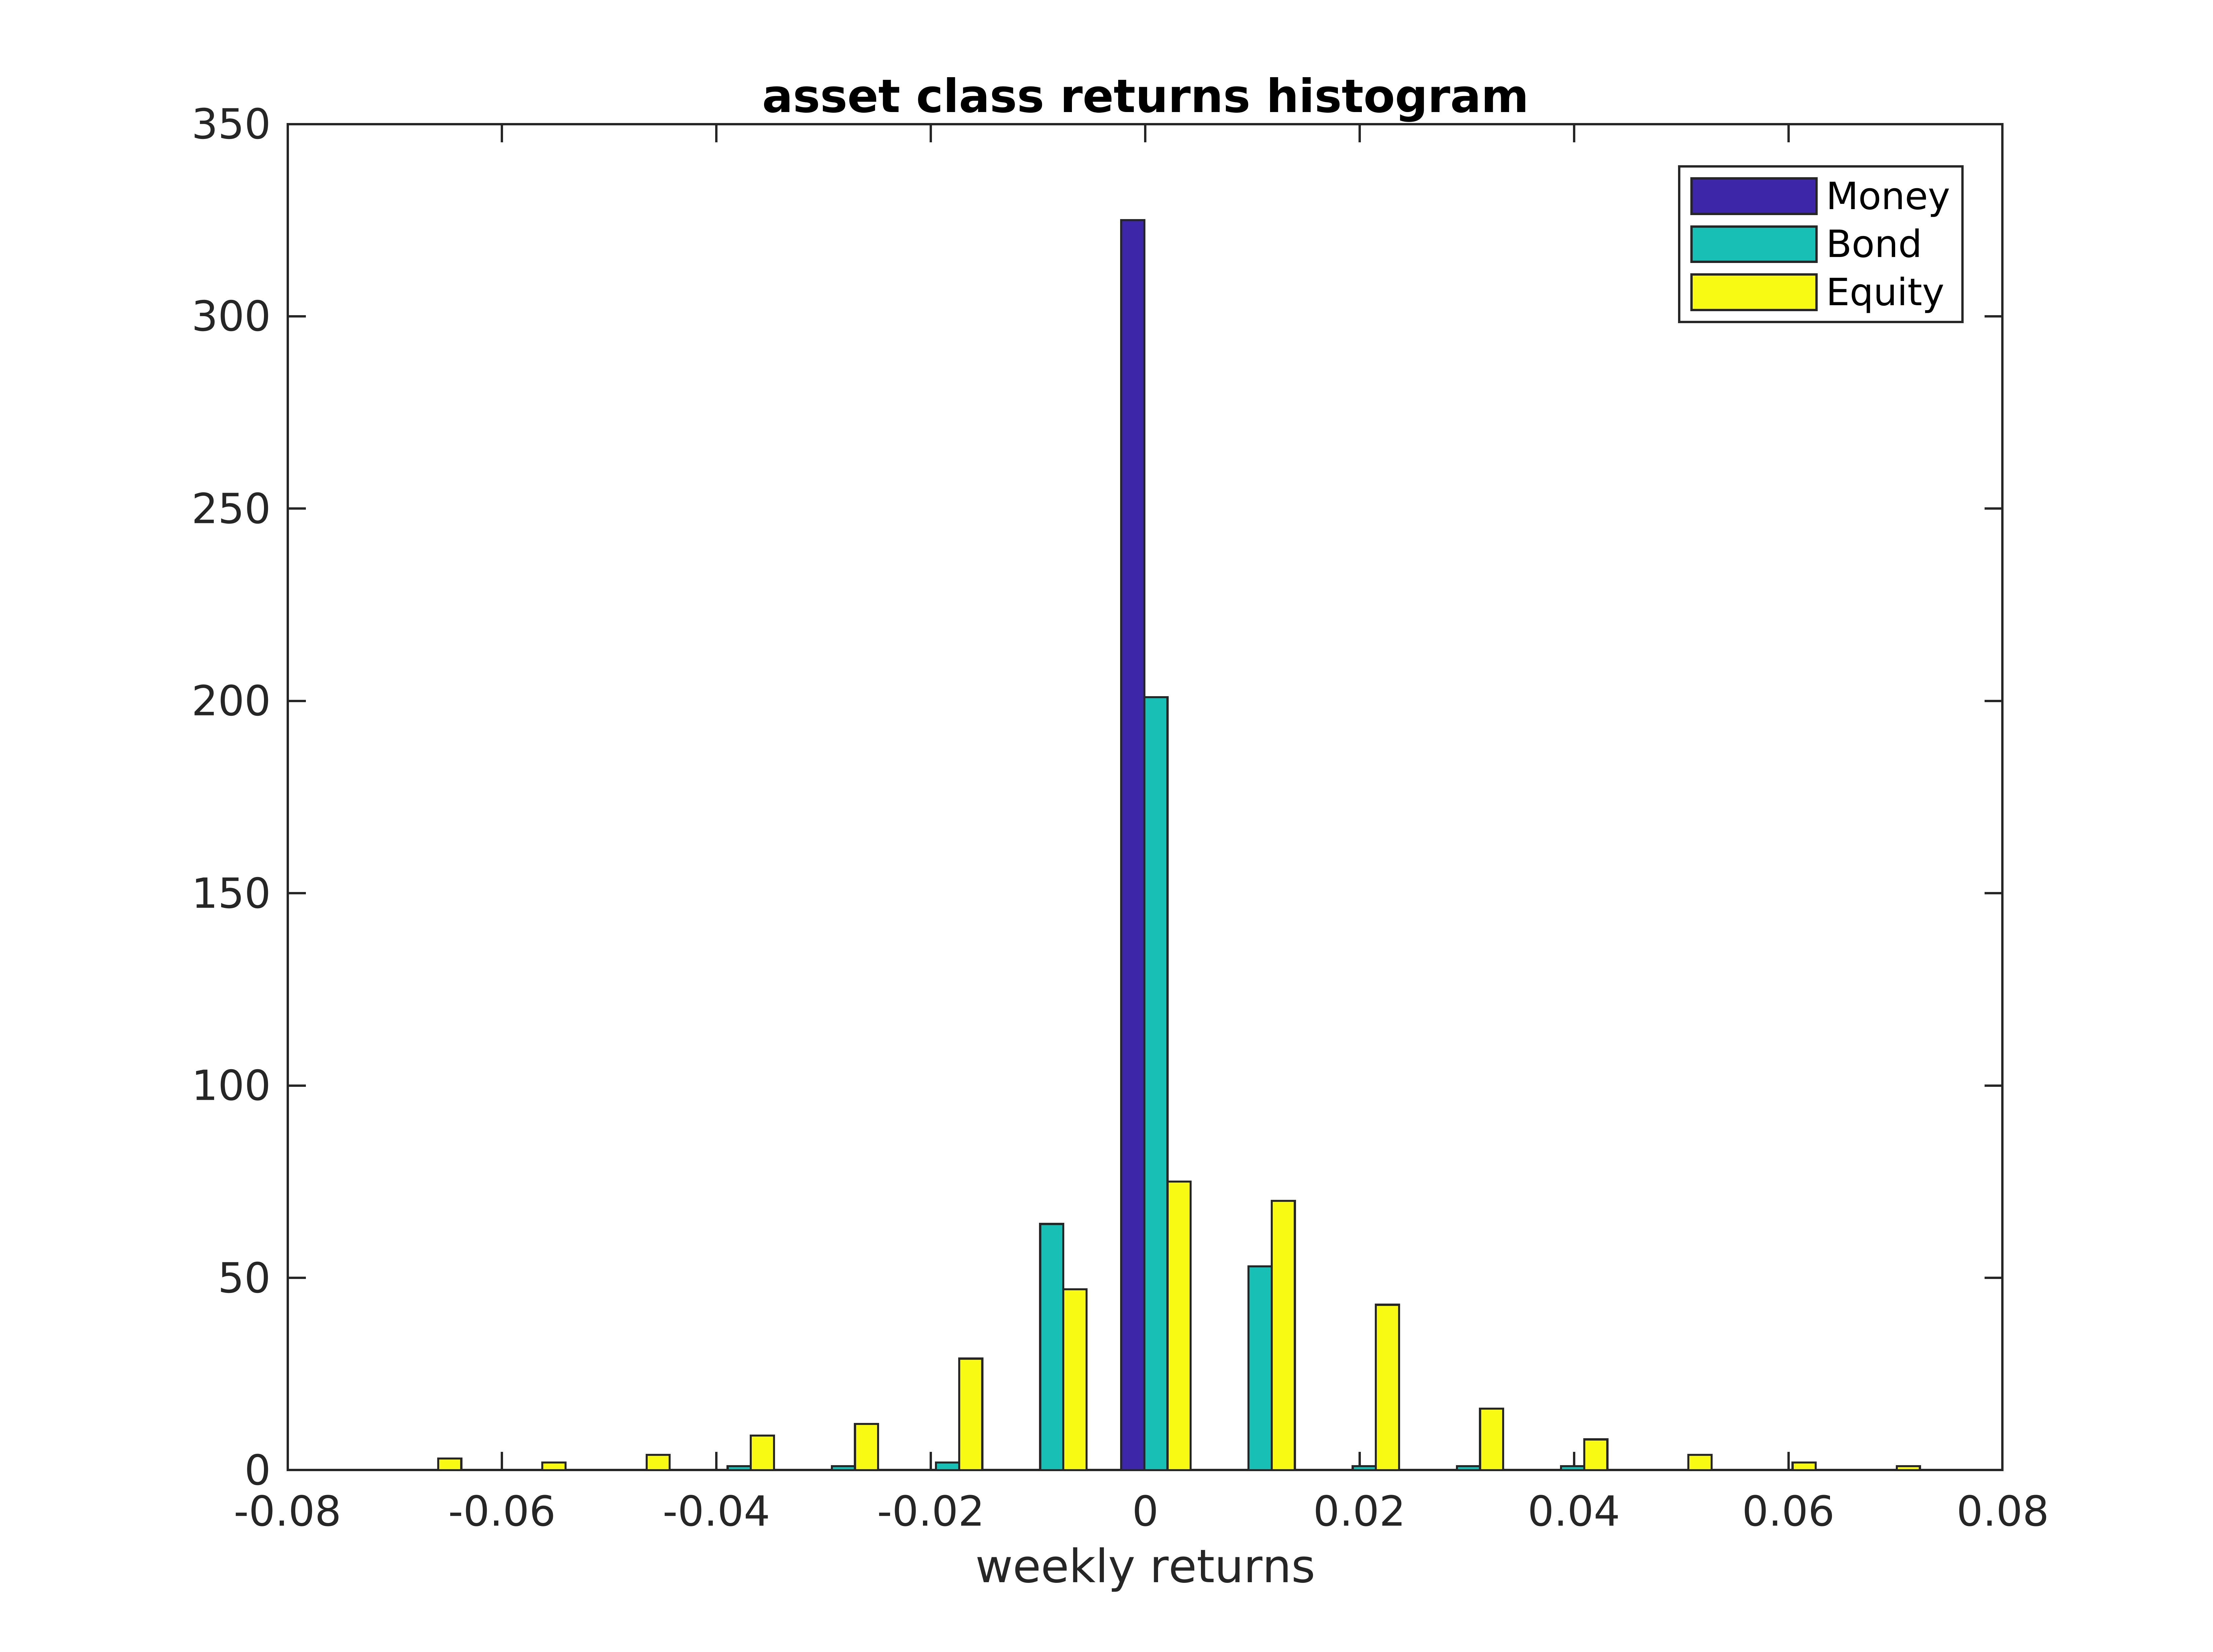
\includegraphics[scale=0.6]{Images/ReturnsHist.png}
	\caption{Weekly asset class returns histogram.}
\end{figure}
\begin{table}[h]
	\centering
	\begin{tabular}{@{}llll@{}} \toprule
		Statistic & C & B & E \\ \midrule
		Mean Return (ann) & 0.064\%  & 3.46\% & 12.11\%\\
		\addlinespace[0.5em]
		Volatility (ann) & 0.113\%  & 4.81\% & 14.81\% \\
		\addlinespace[0.5em]
		Median (ann) &	0\% & 4.58\% & 17.74\% \\
		\addlinespace[0.5em]
		Skewnwss & 0.262 & -0.0621 & -0.36 \\
		\addlinespace[0.5em]
		Kurtosis & 3.90 & 10.62 & 4.42 \\
		\addlinespace[0.5em]
		Monthly $V@R_{0.95}$ & 0.0808\% & 3.73\% & 14.95\%\\
		\addlinespace[0.5em]
		Max Drawdown & 0.106\% & 5.87\% & 23.98\% \\
		\addlinespace[0.5em]
		Mean Drawdown & 0.020\% & 1.5\% & 4.62\% \\
		\addlinespace[0.5em]
		Sharpe ratio & 0 & 0.692 & 0.767 \\ \bottomrule
		\addlinespace[0.5em]
	\end{tabular}
	\caption{Asset class returns sample statistics}
	\label{tab:sampleStatistics}
\end{table}

Finally, the sample correlation matrix is  
\[ 
\begin{bmatrix}
1 & 0.166 & -0.075 \\
  &  1    & -0.454 \\
  &       &  1
\end{bmatrix}.
\]

\section{Optimal Allocation Maps}\label{sec:Allocation_Maps}
Let us consider an asset allocation problem characterized by the following parameters:
\begin{itemize}
	\item 2-year investment horizon
	\item weekly rebalancing frequency, which means $N=104$ portfolio rebalancings
	\item monthly value-at-risk equals to 7\%
	\item target return $\theta=7\%$ per year
	\item initial wealth $x_0 = 1$
\end{itemize}
The target sets we want our portfolio value to stay within are 
\begin{align*}
X_0 & = \{1\}\\
X_k & = [0,\infty) \quad k = 1,\ldots,103 \\
X_{104} & = [(1+\theta)^2,\infty) = [1.07^2,\infty)
\end{align*}
In practice, these sets are discretized with a discretization step of $10^{-3}$ and truncated where the probability measure is negligible; the actual sets used in the implementation thus are $X_k = [0.5,1.9]$ $k=1,\ldots,103$, $X_{104}=[(1.07)^2,1.9]$. As stated in Problem \ref{prb:ODAA}, we are looking for a sequence of allocation maps which maximize the following joint probability
\[ \mathbb{P}\big(\{\omega \in \Omega : x_0 \in X_0,\ldots,x_{104} \in X_N \} \big).\]
The final choice to be made before running the algorithm is picking a model for the asset class returns. As a first example, we opt for the GM model which has been fitted to data applying the Expectation-Maximization method (see Subsection \ref{subsec:EM}). The parameter estimates are:

\begin{align}
\label{eq:GMparam1}
\bm{\mu}_1 & = 
\begin{bmatrix}
\num{1.054e-5} \\
\num{3.713e-4} \\
\num{2.298e-3}
\end{bmatrix}
\quad & \bm{\Sigma}_1 &= 
\begin{bmatrix}
\num{2.437e-8} & \num{1.266e-7} & \num{-2.365e-7} \\
& \num{3.596e-5}  & \num{-5.944e-5} \\
&                & \num{4.232e-4}
\end{bmatrix} \\
\bm{\mu}_2 & = \begin{bmatrix}
\num{2.115e-4} \\
\num{3.105e-2} \\
\num{-8.266e-3}
\end{bmatrix}
\quad & \bm{\Sigma}_2 &= 
\begin{bmatrix}
\num{2.372e-8} & \num{-7.961e-7} & \num{1.277e-6} \\
& \num{2.9e-5}  & \num{-4.411e-5} \\
&                & \num{6.949e-5}
\end{bmatrix}
\label{eq:GMparam2}
\end{align}
and $\lambda = 0.9908$.
By applying the backward algorithm enunciated in Theorem \ref{thm:rec_algo} we obtained 103 allocation maps, some of which are reported in Figure \ref{fig:mapsMixture}.
\begin{figure}[]
	\makebox[\textwidth][c]{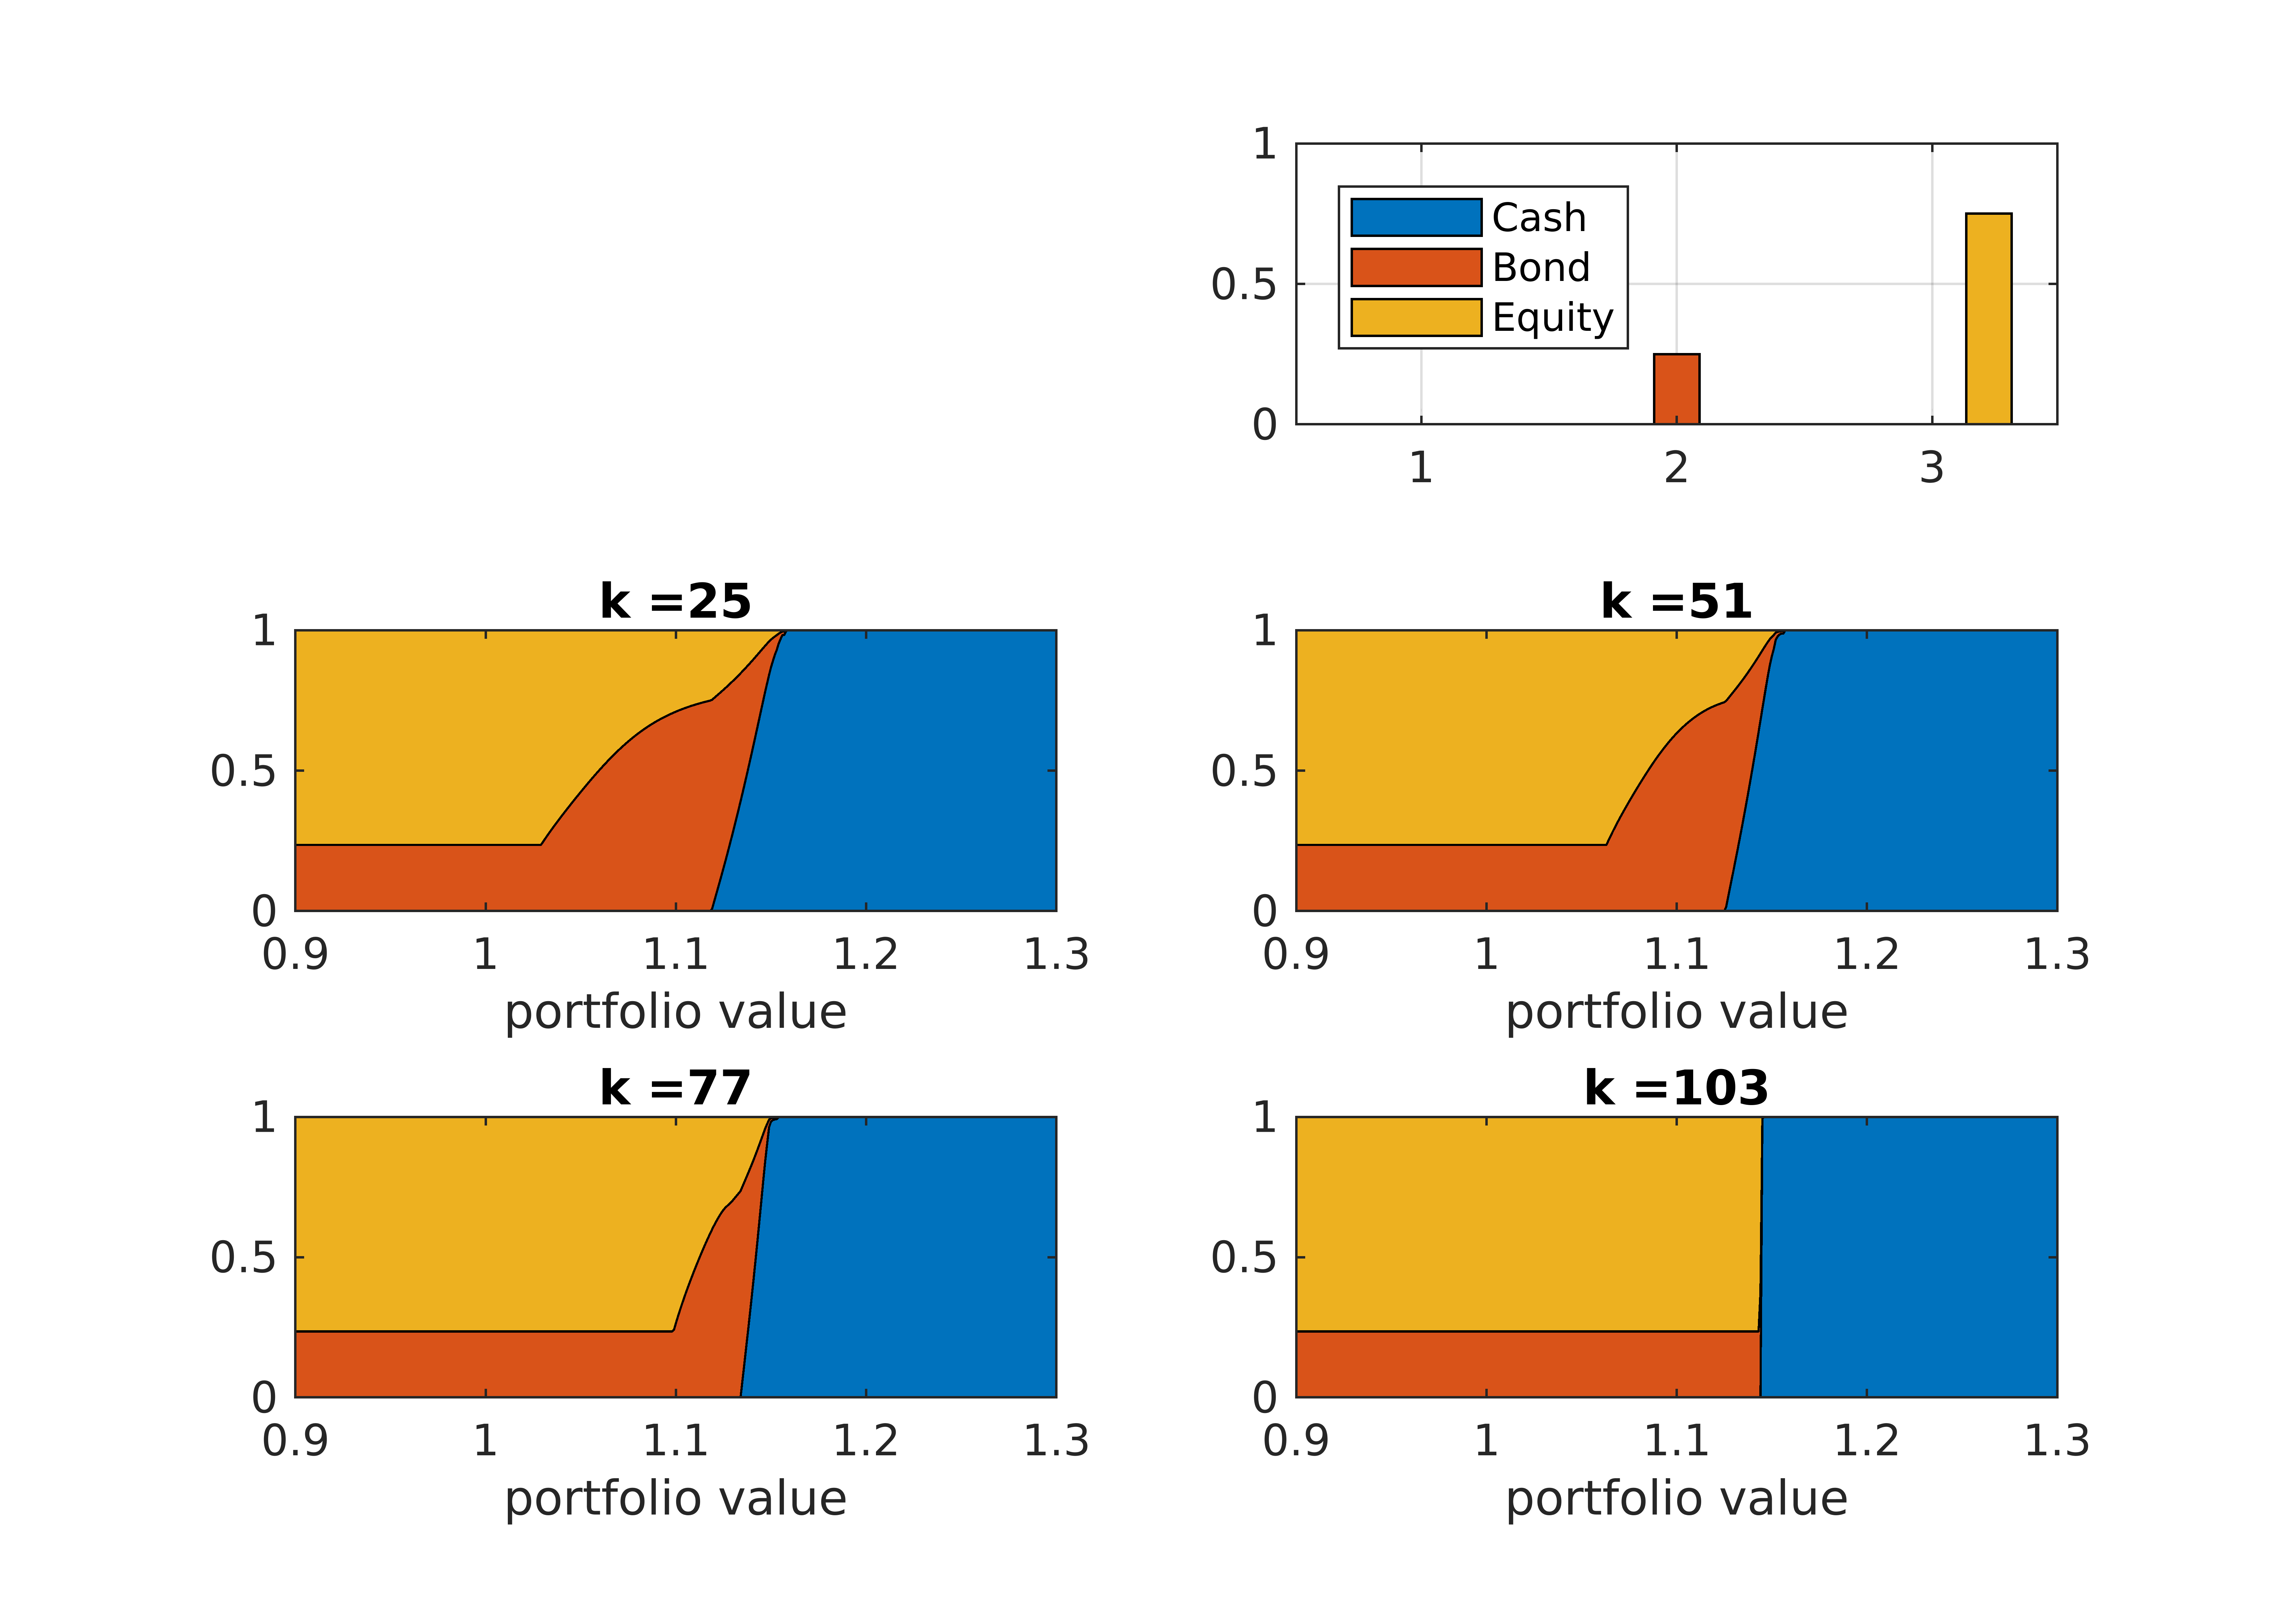
\includegraphics[scale =1]{Images/mapsMixturewk.png}}
	\caption{Optimal allocation maps, weekly rebalancing, GM model}
	\label{fig:mapsMixture}
\end{figure}


Let us now take the time to analyze the kind of investment strategy these maps imply. At the beginning of the investment ($k=0$), the optimal strategy prescribes that 25\% of investor's wealth be invested in Bond and 75\% in Equity. After 25 weeks, depending on the realization of portfolio value (x-axis in Figure \ref{fig:mapsMixture}), the optimal strategy tells us to allocate wealth as follows: if the portfolio is underperforming (e.g. its value is approximately below 1.029), the optimal allocation is a mix of Equity and Bond, that is the riskiest mix allowed (a 100\% allocation in Equity is not permitted due to the \text{risk} constraint). As soon as performance gets better (i.e. from \$1.029 to \$1.16) the Equity weight decreases in favor of more Bond and from a certain point on also Cash. When the portfolio is outperforming (i.e. above \$ 1.16), the whole wealth is invested in Cash, namely the least risky of the three asset classes. This kind of investing strategy is known in the literature with the name of \textit{contrarian} strategy. The name stems from the fact that contrarian investors bet against the prevailing market trend, namely they try to sell "high" and buy "low". Contrarian strategies perform well in volatile markets and poorly in trending market due to their \textbf{concave} nature (see \cite{Perold1988}). The optimal strategy obtained by the ODAA algorithm exhibits the same pattern also at successive rebalancing times, the only difference is that it becomes more extreme while approaching the investment end; for instance, at time $k=103$ there is no transition from the riskiest allocation to the least risky one. This behavior could be synthesized by saying that if the target has not been reached before the last week, the strategy will do whatever it takes to get there by assuming the riskiest exposure.

 The joint probability of reaching investor's goal is $J(x_0) = p^{\star} = 78.72\%$. This result is verified by running a Monte-Carlo simulation with $10^5$ draws at each rebalancing period from a GM distribution with parameters \ref{eq:GMparam1} and \ref{eq:GMparam2}, the joint probability obtained is $p_{MC} = 78.73\%$. Another interesting feature of the ODAA strategy is that $p^{\star}$ increases as the rebalancing frequency decreases. By looking at Table \ref{tab:ODAA_results}, it can be seen that as we move from a quarterly rebalancing frequancy\footnote{the problem of switching from a rebalancing frequency to another has been tackled as follows: the model is calibrated to weekly data, then linear returns are approximated by log-returns enabling us to write additive relations such as $w_{monthly} = w_{wk1}+\ldots+w_{wk4}$. Finally, using the hypothesis if iid returns we analytically derive the distribution of monthly and quarterly returns for the G, GM and NIG model. All this models are closed under convolution. } to a monthly one the optimal probability goes from 69.52\% to 73.35\%, and the same happens from monthly to weekly. This fact is rather intuitive since the more rebalancings the more chances to steer the portfolio within the target sets. It should be noted however, that in practice transaction costs have not a negligible impact on portfolio profitability when rebalancing is frequent. This is the reason why investment policies that update portfolio weights only when an "event" occurs are particularly appealing (they will be treated in Part \ref{part:2}).
 
 
\begin{table}[]
	%\renewcommand{\arraystretch}{0.5}
	\centering
	\resizebox{\textwidth}{!}{\begin{tabular}{@{}*{10}{c}@{}}
		\toprule
		& \multicolumn{3}{c}{G} & \multicolumn{3}{c}{GM} & \multicolumn{3}{c}{NIG} \\
		\addlinespace[0.5em]
		\cmidrule(l){2-4} \cmidrule(l){5-7} \cmidrule(l){8-10} 
		& wk & m & q 	& wk & m & q 	& wk & m & q\\
		\addlinespace[0.5em]
	$p^{\star}$ & 79.67\% & 75.56\% & 73.26\% & 78.59\%  & 73.20\% & 69.44\% & 78.53\% & 73.24\% &69.47\%  \\
	\addlinespace[0.5em]
	$p_{MC}$ & 79.77\% & 75.56\% & 73.28\% & 78.82\%  & 73.21\% & 69.58\% & 78.76\% & 73.30\% &69.32\%  \\
	\addlinespace[0.5em]	
	time[h] & 0.712 & 0.157 & 0.050 & 0.857  & 0.316 & 0.283 & 6.131 & 1.467 &0.371  \\	\bottomrule
	\end{tabular}}
	\caption{Probability of reaching the target set obtained via  ODAA algorithm ($p^{\star}$) and Monte-Carlo simulation ($p_{MC}$) for the Gaussian (GM), Gaussian Mixture (GM) and Normal Inverse Gaussian (NIG) model. Time is the computational time of the ODAA algorithm in hours.}
	\label{tab:ODAA_results}
\end{table}

\begin{table}[]
	\centering
	\begin{tabular}{@{}*{4}{c}@{}}
		\toprule
		& G & GM & NIG \\
		%\addlinespace[0.5em]
		\midrule	
		$\log L^{\star}$ & 4396.2& 4455.0  & 4481.4\\
		\addlinespace[0.5em]	
		\bottomrule
	\end{tabular}
	\caption{Log-likelihood for G, GM and NIG model}
	\label{tab:LogL_models}
\end{table}

Next, we used also the Gaussian and the NIG model to describe the asset class returns distribution. From Table (\ref{tab:LogL_models}) we see that the best fitting is provided by the GM model since it exhibits the highest Log-likelihood function value, nonetheless the NIG comes right after it. It is not surprising that the Gaussian model is ranked last as we were well-aware that the data considered deviates from a multivariate Gaussian sample (see Table \ref{tab:sampleStatistics}).
%\begin{wraptable}{l}{6cm}
%	\centering
%	\begin{tabular}{@{}*{5}{c}@{}}
%		\toprule
%	Moment	& G & GM & NIG & Empirical\\
%		\addlinespace[0.5em]
%		\midrule	
%	$\mu_{x_{k+1}}$	& & & \\
%	\addlinespace[0.5em]	
%	$\sigma_{x_{k+1}}$	& & & \\
%	\addlinespace[0.5em]
%	$\gamma_{x_{k+1}}$	& & & \\
%	\addlinespace[0.5em]
%	$\kappa_{x_{k+1}}$	& & & \\
%	\addlinespace[0.5em]
%	\bottomrule
%	\end{tabular}
%\end{wraptable}


\subsection{ODAA vs CPPI vs Constant-Mix}
Within the class of asset allocation strategies, the \gls{CPPI} and the Constant-Mix are among the most popular ones (see \cite{Perold1988}). After briefly discussing how they work, we will compare their performance to the ODAA's one.
\paragraph{CPPI}
The idea behind the \gls{CPPI} is to maintain the portfolio \textbf{exposure} to the risky asset, $E_k$, a constant multiple $m$ of the portfolio \textbf{cushion}, $C_k$. The risky asset is assume to be a mix of Bond and Equity. The cushion at time $k$ is defined as
\[
C_k = \max\big\{x_k-F_k,0 \big\}
\]
where $x_k$ is the portfolio value at time $k$ and $F_k$ is the so-called portfolio \textbf{floor}. The floor is a value below which the investor does not want the portfolio value to fall. In our case, the floor is a risk-free asset which grows deterministically at the Cash rate. Therefore, once the investor has specified 
\begin{itemize}
	\item an initial allocation $\bm{u}_0$ 
	\item the initial floor $F_0$ 
	\item a cushion multiplier $m$
	\item the maximum value-at-risk ($V@R_{1-\alpha}$) according to his risk profile,
\end{itemize}
he can synthesized the \gls{CPPI} strategy as follows
\begin{equation*}
\begin{aligned}
& \underset{\bm{u}_k}{\text{maximize}} & &  A\bm{u}_k \\
& \text{subject to} & & \bm{u}_k^T\bm{1}=1, \\
& & & u_i \geq 0 \qquad \forall i \in \{1,2,3\},\\
& & &\bm{u}_k\bm{\Lambda}\bm{u}_k \leq \sigma_{max}^2,\\
& & & \underbrace{xA\bm{u}_k}_{E_k} \leq mC_k.
\end{aligned}
\end{equation*}
where $A=\begin{bmatrix}0 & 1 & 1\end{bmatrix}$, $\sigma_{max}=\frac{V@R_{1-\alpha}}{z_{1-\alpha}}$, $x \in X_k$ and $k = 1,\ldots,N$. From this formulation we see that the investor aims at maximizing the allocation in the risky asset (matrix $A$ selects the allocation in Bond and Equity) while keeping under control the riskiness of the overall allocation and limiting the risky exposure to $m$ times the cushion. The covariance matrix $\bm{\Lambda}$ depends on the model chosen to describe the asset class returns distribution. In our analysis, we set $m=6$, $\bm{u}_0$ equal to the initial ODAA allocation, $F_0$ is chosen in such a way that also the initial exposure is $m$ times the cushion and the asset class return random vector follows a GM distribution with parameters (\ref{eq:GMparam1}) and (\ref{eq:GMparam2}). The others investment parameters are equal to the ones in the ODAA case. The CPPI allocation maps are reported in Figure \ref{fig:mapsMixtureCPPI}.



\paragraph{Constant-Mix}
Following a Constant-Mix strategy means maintaining an exposure to the risky asset that is a constant proportion of wealth. For instance, suppose one decides to keep a 60/40 proportion between risky ans risk-free asset. After a rebalancing time, asset prices change causing the portfolio proportion to change as well. Let us suppose that the risky asset has increased its price while the risk-free has fall. At the next rebalancing time, the Constant-Mix policy prescribes to sell shares of the risky asset and buy shares of the risk-free in order to recover the 60/40 mix. The constant mix is chosen by solving the following equivalent formulation of the Markowitz problem
\begin{equation*}
\begin{aligned}
& \underset{\bm{u}}{\text{maximize}} & &  \bm{u}^T\bm{\mu} \\
& \text{subject to} & & \bm{u}^T\bm{1}=1, \\
& & & u_i \geq 0 \qquad \forall i \in \{1,2,3\},\\
& & &\bm{u}\bm{\Lambda}\bm{u} \leq \sigma_{max}^2.\\
\end{aligned}
\end{equation*}
where $\sigma_{max}=\frac{V@R_{1-\alpha}}{z_{1-\alpha}}$ and $\bm{\mu}$ and $\bm{\Lambda}$ are the mean and the covariance matrix of the random vector $\bm{w}_{k+1}$ which represents the asset class returns.
The distribution of $\bm{w}_{k+1}$ could be any of the ones discussed in Chapter \ref{chpt:assetclass_returns}. The optimization problem has been solves assuming a GM distribution with parameters (\ref{eq:GMparam1}) and (\ref{eq:GMparam2}); the optimal constant mix is
\[ \bm{u}^{\star} = \begin{bmatrix} 0 & 0.2352 & 0.7648 \end{bmatrix}^T.\]


The ODAA and Constant-Mix belongs to the \textbf{concave} allocations strategies (see \cite{Plasse2013}). This means that their policy is to buy risky assets (Equity and Bond) when they fall and sell them when they raise. Concave strategies perform well in oscillating markets. Conversely, the \gls{CPPI} is an example of a \textbf{convex} strategy: risky assets are bought when they raise and sold when they fall. This behavior is clear from the allocation maps in Figure \ref{fig:mapsMixtureCPPI}. When portfolio performance is up, a more risky position is taken, when it is down, risky assets are sold and a more covered position is taken. Convex strategies perform well in trending markets.

In order to compare the performance of this three different strategies we ran a Monte-Carlo simulation. Starting from an initial wealth $x_0=1$, $\num{2e5}$ portfolio trajectories are drawn assuming a GM distribution with parameters (\ref{eq:GMparam1}) and (\ref{eq:GMparam2}) for vectors $\bm{w}_{k+1}$. Performance and risk figures are reported in table \ref{tab:MC_statistics}. The empirical density function of the 2-year investment return is reported in Figure \ref{fig:epirical_densities}.








\begin{figure}[]
	\makebox[\textwidth][c]{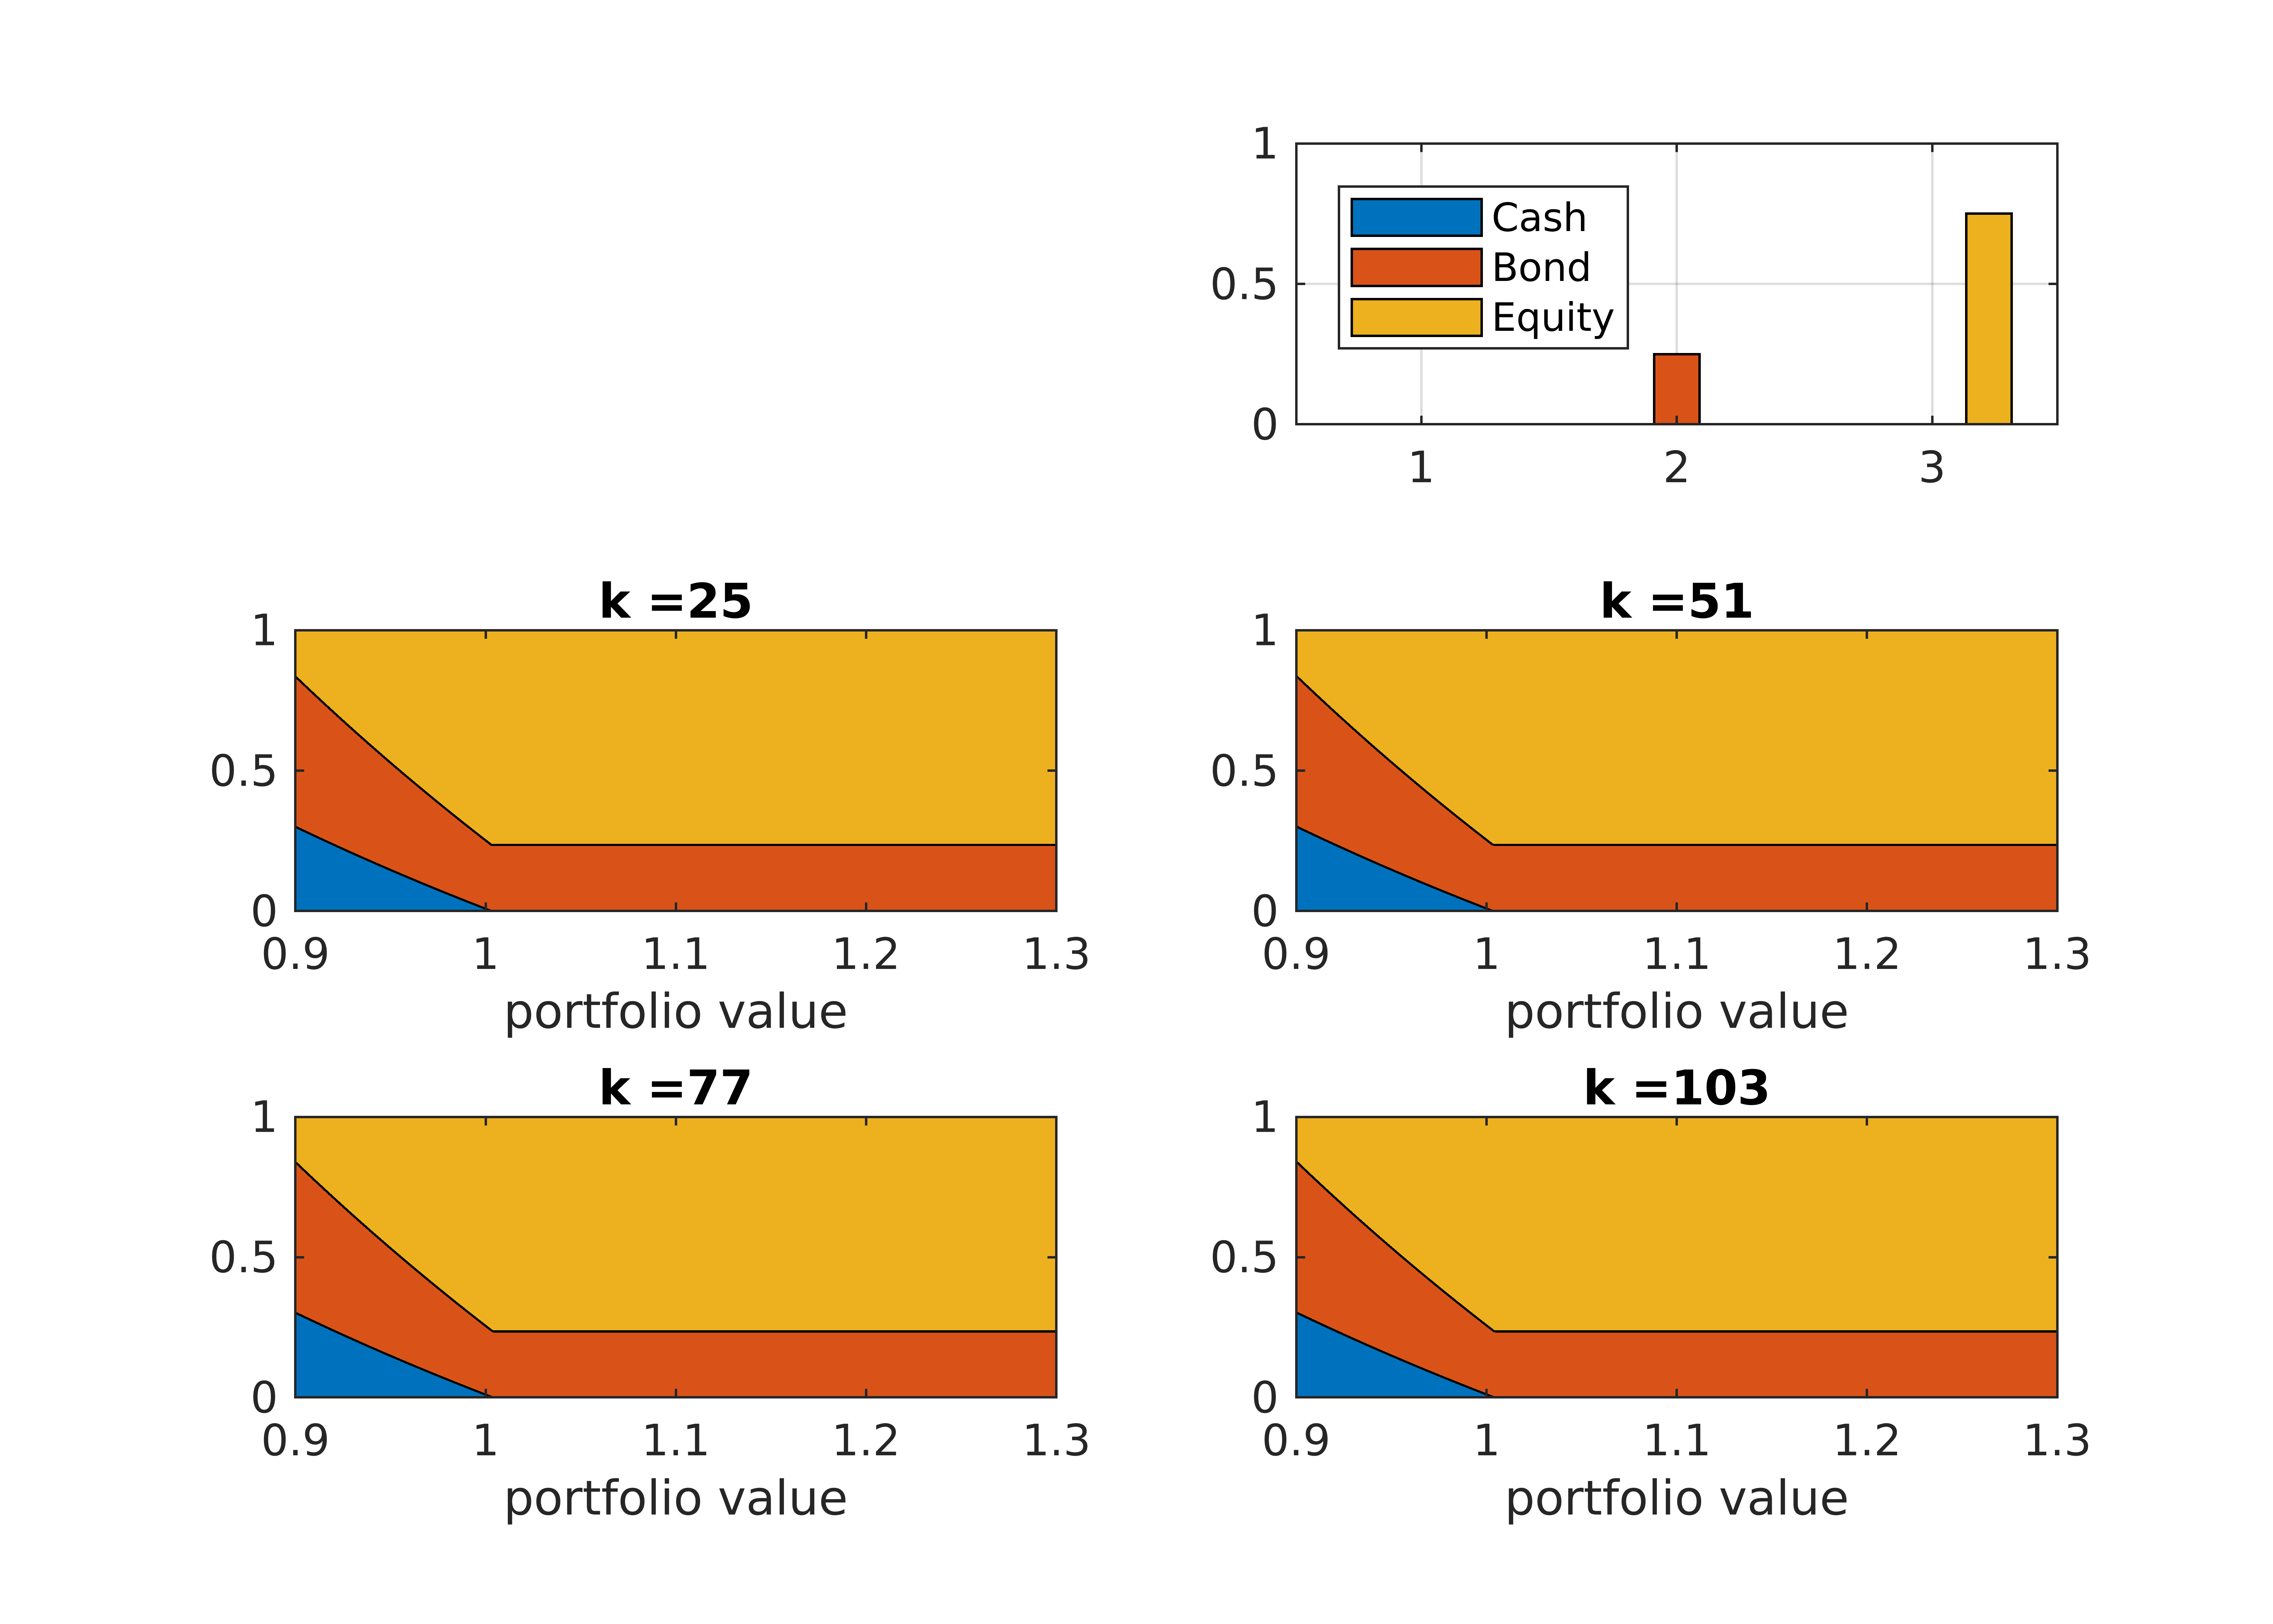
\includegraphics[scale = 0.8]{Images/mapsCPPIMixturewk.png}}
	\caption{Optimal CPPI allocation maps, weekly rebalancing, GM model. An example of a convex strategy.}
	\label{fig:mapsMixtureCPPI}
\end{figure}


\begin{table}[]
	\centering
	\begin{tabular}{@{}lccc@{}} \toprule
		Statistic & ODAA & CPPI & Constant-mix \\ \midrule
		$p_{MC}$ &  78.93\%    &  52.70\%    &  61.41\%    \\
		\addlinespace[0.5em]
		Mean Return (ann) & 5.82\%  & 7.55\% & 10.05\%\\
		\addlinespace[0.5em]
		Volatility (ann) & 5.00\%  & 7.93\% & 13.21\% \\
		\addlinespace[0.5em]
		Median (ann) &	7.20\% & 7.35\% & 9.41\% \\
		\addlinespace[0.5em]
		Skewnwss & 0.700 & -0.010 & 0.0146 \\
		\addlinespace[0.5em]
		Kurtosis & 6.700 & 3.052 & 3.012 \\
		\addlinespace[0.5em]
		Monthly $V@R_{0.95}$ & 5.49\% & 5.51\% & 9.42\%\\
		\addlinespace[0.5em]
		Max Drawdown & 43.39\% & 25.77\% & 45.80\% \\
		\addlinespace[0.5em]
		Mean Drawdown & 1.97\% & 2.12\% & 4.20\% \\
		\addlinespace[0.5em]
		Sharpe ratio & 1.163 & 0.951 & 0.760 \\ \bottomrule
		\addlinespace[0.5em]
	\end{tabular}
	\caption{Investment performance for strategies ODAA, CPPI and Constant-mix obtained via Monte-Carlo simulation ($\num{2e5}$ replications).}
	\label{tab:MC_statistics}
\end{table}



\begin{figure}[]
	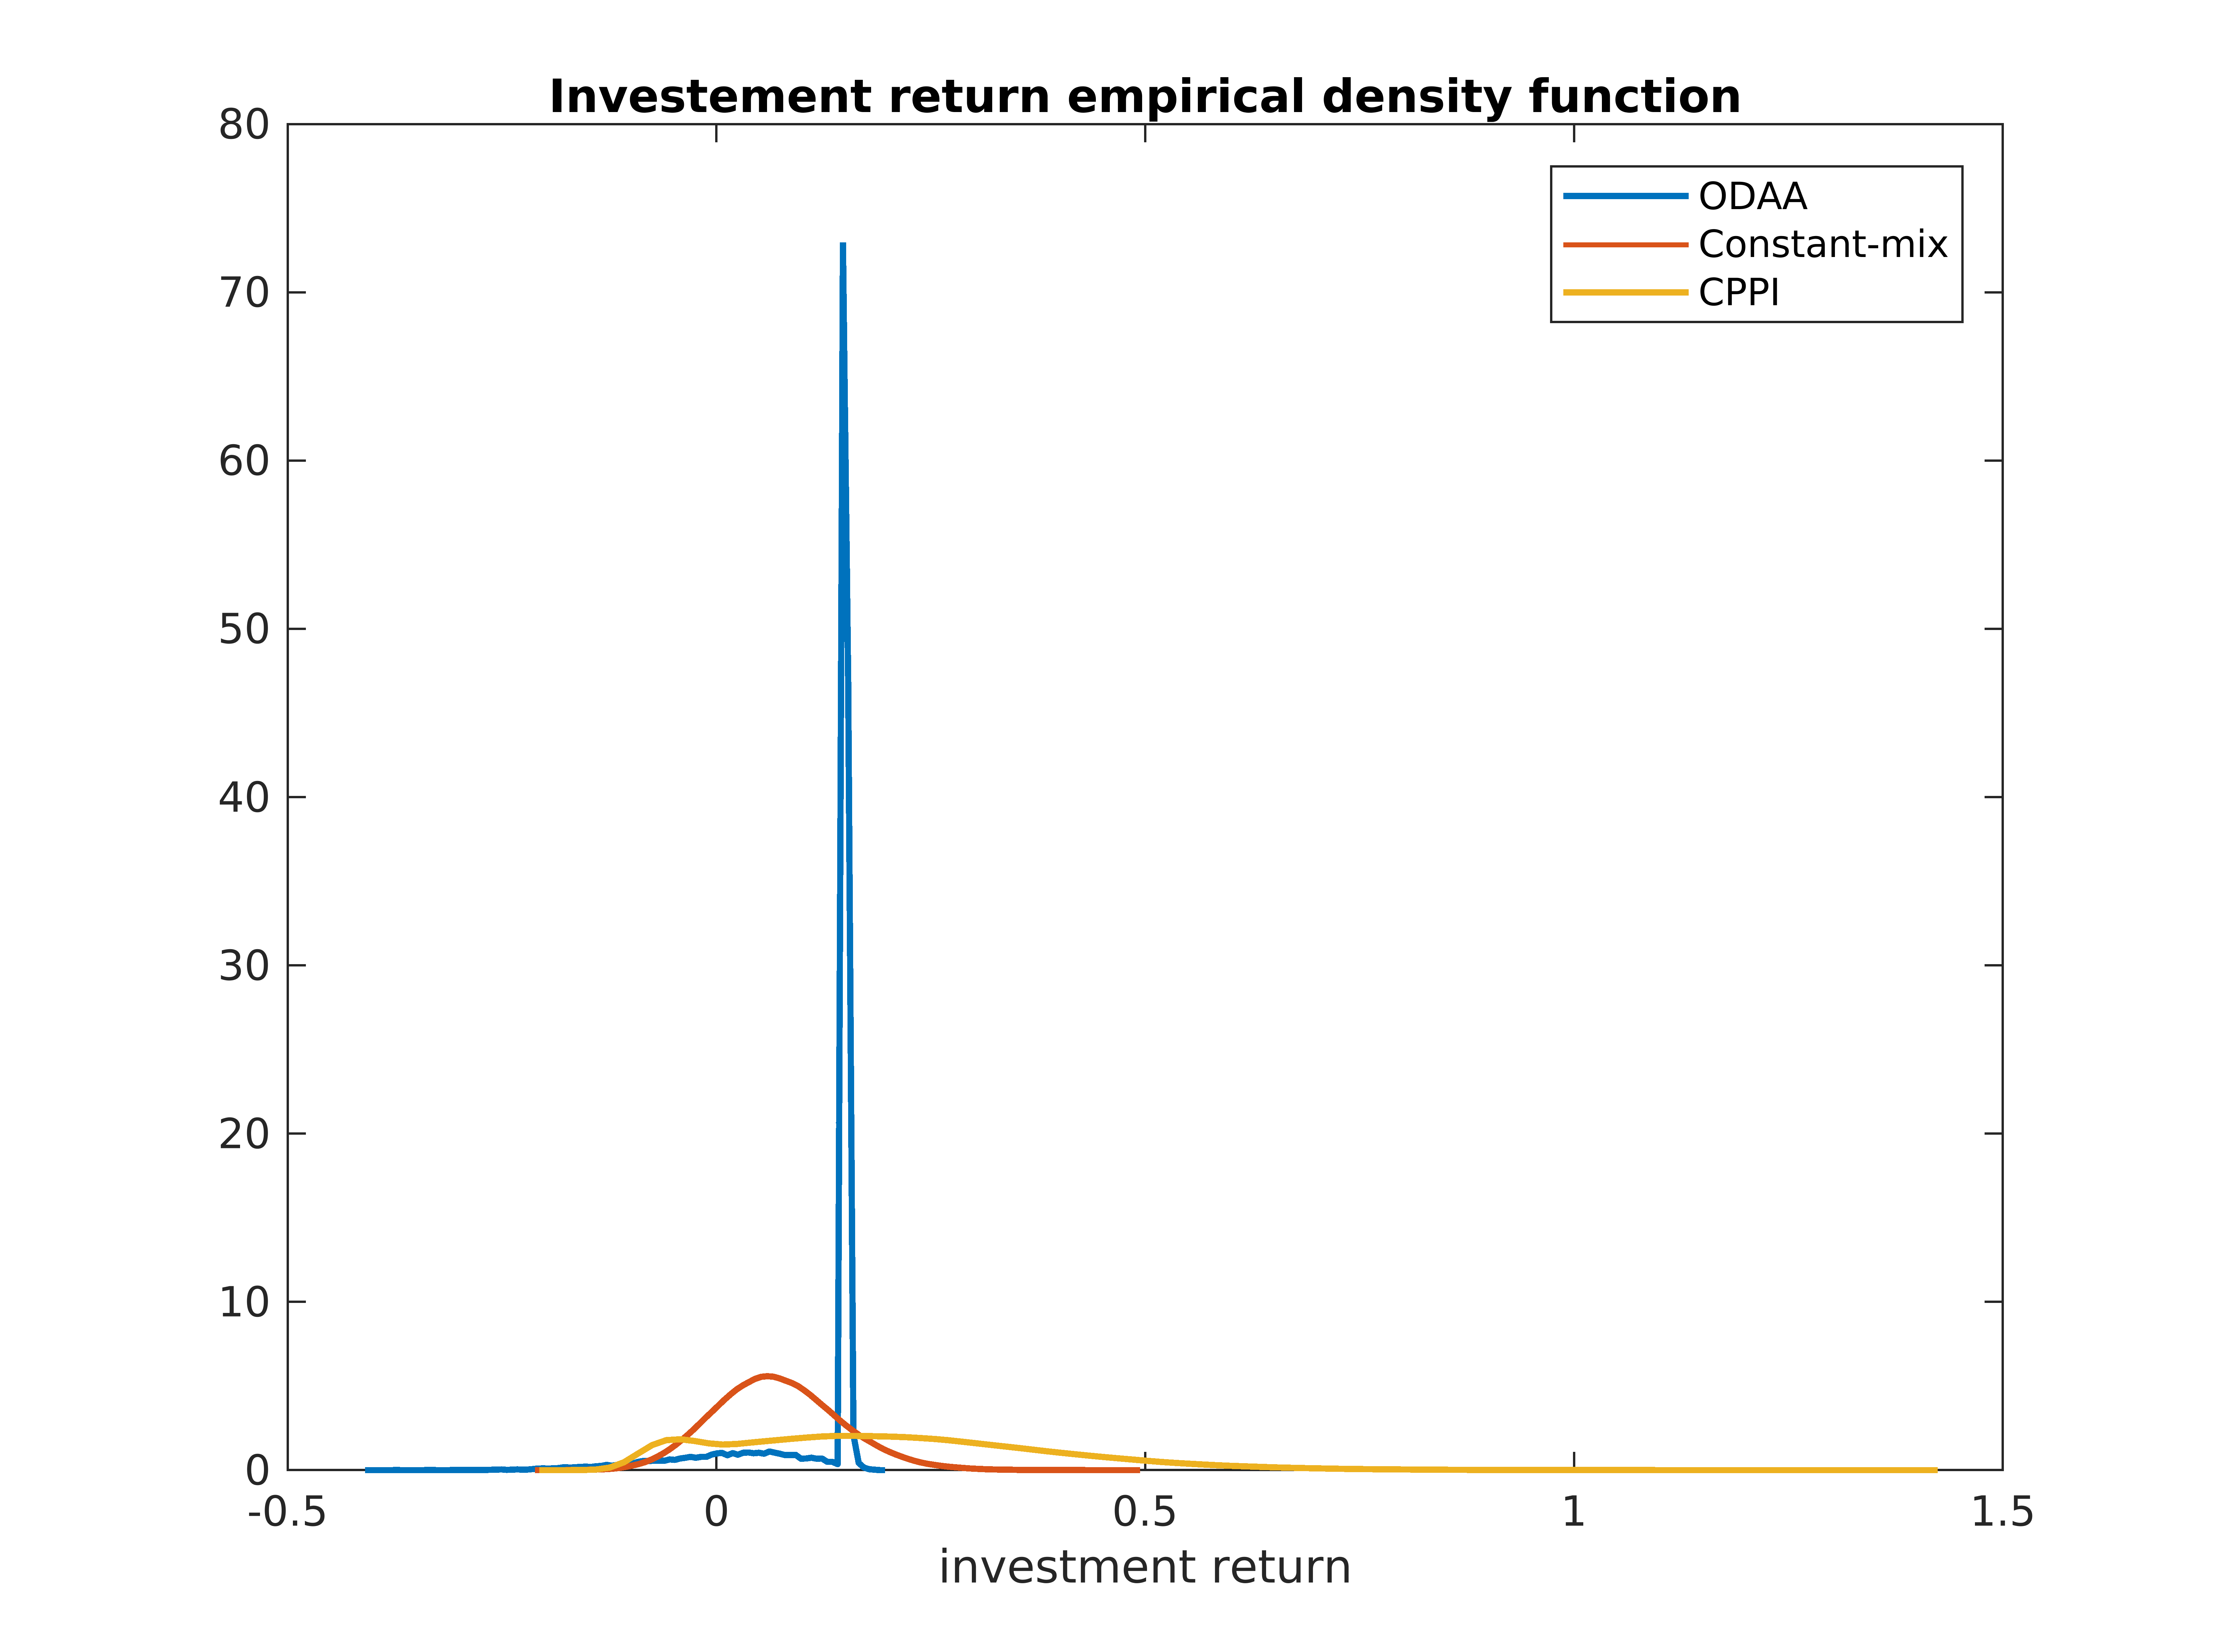
\includegraphics[scale = 0.6]{Images/DensitiesMixturewk}
	\caption{Empirical density functions of the 2-year return for the ODAA, CPPI and Constant-ix strategy.}
	\label{fig:epirical_densities}
\end{figure}

\part{Event-Driven approach}\label{part:2}

\chapter{Discrete Event Systems and Asset Allocation}\label{chpt:ED}
From this chapter on, we will adopt a different approach to the asset allocation problem: time will no longer be the driver of portfolio rebalancing but instead portfolio weights  will be updated whenever a predefined \textbf{event} occurs. This new point of view stems from the fact that when developing the stochastic reachability approach in Chapter \ref{chpt:Model_Description}, we let the system dynamics be indexed by an independent variable $k \in \mathbb{N}$ which we interpreted as discrete time but, as a matter of fact, the theory did not rely on this particular interpretation. This gives us the freedom to think of $k$ as an abstract index (for instance it could be an event counter). This observation is the basis for embedding the asset allocation problem in a \gls{DES} environment. 

In this chapter we will present the basics of \gls{DES} modeling (Section \ref{sec:Introduction_to_DES}) which are essential for discussing the \gls{ED} approach to asset allocation (Section \ref{sec:EventDrivenAA}). As far as the \gls{DES} is concerned, the main reference is the rich monograph \cite{cassandras2009}, whereas the \gls{ED} asset allocation model is taken from \cite{specchio2011}.

\section{Introduction to DES }\label{sec:Introduction_to_DES}
From a Control System point of view, the dynamical system introduced in (\ref{eq:state_equation}) can be classified as \textit{continuous-state} (the state space $\mathcal{X}$ is a proper subset of $\mathbb{R}$) and \textit{discrete-time} ($k \in \mathbb{N}$). Informally, if the state space is a discrete set and state transitions are observed whenever an "event" occurs we will talk about Discrete Event Systems. Systems considered so far are time-driven, in that we could imagine the systems being synchronized to a clock and at every clock tick an event $e$ is drawn from an event space $E$ causing the state to change. However, we could think of a different mechanism governing the state transition: at various time instants (not necessarily known in advanced), some event $e \in E$ occurs, making the state change.
The following example will hopefully clarify the difference between \gls{TD} and \gls{ED} systems. Imagine a particle bound to move on a plane; at every tick of a clock an event is drawn and the particle is allowed to move by a unit step in direction North, South, East or West. In this case we have a \gls{TD} system whose events are $e_1= \text{"one step North"}$, $e_2= \text{"one step South"}$ and so on. On the other hand, suppose there are four players, each of them capable of making the particle move in his direction by issuing a signal. A player issues a signal at random times. The resulting system is \gls{ED} since it is not synchronized to any clock and state transitions are caused by event like $e_k=$"player 1 issued a signal". The formal definition of a \gls{DES} reads as follows
\begin{definition}[Discrete Event System]
	A \textbf{Discrete Event System} is a \textit{discrete-state}, \textit{event-driven} system, that is, its state evolution depends entirely on the occurrence of asynchronous discrete events over time.
\end{definition} 


A \gls{DES} can be studied from three different levels of abstraction. We will present them in increasing order of complexity
\begin{enumerate}
	\item \textit{untimed}: the interest is on the sequences of events that the system could execute, without any time information. For instance, an untimed sequence could be
	\[e_1, e_2, e_3, e_4, e_5, e_6 \]
	\item \textit{timed}: in this representation each possible event sequence is coupled with time information, that is, not only the order of occurrence is given but also the exact time instant an event occurred. For example, in the \textit{timed} setting, the following could be a system sample path
	\[(e_1,t_1), (e_2,t_2), \ldots, (e_6,t_6) \]
	
	
	\item \textit{stochastic timed}: it is the most detailed description of a \gls{DES} since it contains event information on all possible orderings, time information about the exact instant at which the event occurs and also statistical information about successive occurrences.
\end{enumerate}
As our modeling purposes required the stochastic timed level of abstraction, we now give the definition of a \textit{Stochastic Clock Structure} which is the tool used to include time and statistical information to a sequence of events.
\begin{definition}[Stochastic Clock Structure]
	The \textbf{Stochastic Clock Structure} associated with an event set $E$ is a set of CDFs
	\[ \bm{G} = \{G_i \colon i \in E \}   \]
	characterizing the stochastic clock sequences
	\[ \bm{V}_{i} = \{V_{i,1},V_{i,2},\ldots \} \qquad i \in E \]
	where $V_{i,k}$ is a random variable indicating the k-th occurrence time of event $e_i$.
\end{definition}
\begin{remark}
	Sometimes, instead of modeling the exact time when an event occurs (as in the definition above), it is more convenient to model the elapsed time between two events, the so-colled \textbf{interevents time}. In this case we will write the Stochastic Clock Sequence in the following way \[ \bm{T}_{i} = \{T_{i,1},T_{i,2},\ldots \} \qquad i \in E. \]
\end{remark}
If a deterministic clock sequence  $\bm{v}_i = \{v_{i,1}, v_{i,2},\ldots\}$ is given for each event in $E$, we will talk about a \textit{Clock Structure} (this is the case in the \textit{timed} case). The evolution of a \gls{DES} needs to be described by a state equation of the form
\begin{equation}\label{eq:untimed_dynamics}
x_{k+1} = f(x_k,e_{k+1}) \qquad k \in \mathbb{N}
\end{equation}
where $x_k$ is the current state and $x_{k+1}$ the state once the event $e_{k+1}$ has occurred. The above recursive equation is the event-driven equivalent of Equation (\ref{eq:state_equation}). However, Equation (\ref{eq:untimed_dynamics}) describes only the untimed dynamics, that is no time information is included. Conversely, in asset allocation applications, we are interested also in \textit{when} an event occurs. For this reason, after introducing a Clock Structure $\bm{v} = \{v_i \colon i \in E\}$ associated with a finite event set $E = \{e_1,\ldots,e_n\}$, we seek a relationship of the form \[ e_{k+1} = h(x_k,\bm{v}_1,\ldots,\bm{v}_n)\] so that we could replace (\ref{eq:untimed_dynamics}) with
\begin{equation}\label{eq:timed_dynamics}
\begin{cases}
x_{k+1} & = f(x_k,e_{k+1})\\
e_{k+1} & = h(x_k,\bm{v}_1,\ldots,\bm{v}_n).
\end{cases}
\end{equation}
Equations (\ref{eq:timed_dynamics}) capture the \textit{timed} dynamics of a \gls{DES}.

As it was mentioned earlier, the \text{Stochastic timed} behavior is what interests us; therefore, we conclude this section by giving the definition of a Stochastic Timed Automaton which is the theoretical modeling structure of a \gls{DES} (see \cite{cassandras2009} for a more detailed treatment)
\begin{definition}[Stochastic Timed Automaton]
	A \textbf{Stochastic Timed Automaton} is a six-tuple \[ (\mathcal{E},\mathcal{X},\Gamma,p,p_0,\bm{G})\]
	where 
	\begin{description}
		\item[$\mathcal{E}$] is a countable event set
		\item[$\mathcal{X}$] is a countable state space
		\item[$\Gamma(x)$] is the set of feasible events, defined $\forall x \in \mathcal{X}$
		\item[$p(x';x,e')$] is the transition probability from state $x$ to state $x'$ given the occurrence of event $e'$
		\item[$p_0(x)$] is the pmf of the initial state $X_0$ (which is a random variable)
		\item[$\bm{G}=\{\bm{T}_i \colon i \in \mathcal{E}\}$] is a Stochastic Clock Time of interevent times.
	\end{description}
\end{definition}
A Stochastic Timed Automaton, together with the dynamics in Equation (\ref{eq:timed_dynamics}) (where the Clock Structure $\bm{v}$ is replaced by a Stochastic one $\bm{V}$) give the most complete description of a \gls{DES}. We now move to the asset allocation application.
\section{Event-Driven Asset Allocation}\label{sec:EventDrivenAA}
In this section we present the first event-driven model having in mind the objective to invest in the derivative market. In fact, we will consider a market consisting of a \textbf{risky asset} (a future index) and a \textbf{risk-free asset} (a bank account). The event-driven approach aims at modeling the industrial practice of rebalancing the portfolio weights whenever an "event" occurs. In the following, we suppose that an event has occurred every time the absolute value of the risky return hits a threshold (e.g. 7\%). This policy could be beneficial in different aspects:
\begin{enumerate}
	\item in low-volatile markets, when the risky asset price is quite steady, portfolio weights need not to be updated at predefined time instants but only when the market conditions have significantly changed. This cuts down on transaction costs.
	\item in high-volatile markets, when the risky asset price repetitively increases or plummets in a short period of time (shorter than the rebalancing frequency), the event-driven policy can swiftly intervene by changing the portfolio exposure without having to wait the rebalancing time (when the loss could already be substantial).
\end{enumerate}
The main goal of this section is first to derive a proper event-driven dynamics of the portfolio value and then find its density function which will be plugged in the ODAA algorithm.
Let us now start off by investigating both the time-driven dynamics (which will allow us to estimate how long the investment is going to last) and the event-driven dynamics.
\subsection{Time-driven dynamics}
A portfolio rebalancing is performed every time the absolute value of the risky asset cumulative return, starting from an initial baseline, hits a threshold. Let $J$ be this threshold. We suppose the following time-driven discrete dynamics for the risky asset
\begin{equation}\label{eq:time_driven_dynamics}
S_{k+1} = S_k(1 + J N^{\Delta t}_{k+1}) \qquad k \in \mathbb{N}.
\end{equation}
The random variable $N^{\Delta t}_{k+1}$ (which is the k+1-th element of a sequence of iid random variables) takes values in the discrete set $\{1,0,-1\}$ and indicates whether the discrete price process has a positive, negative or null jump at the end of a time interval of length $\Delta t$. If it takes the value 1, the discrete price process $\{S_k\}$ experiences a positive jump at the end of time period $[t_k,t_{k+1}]$, if the value is -1 then the jump is negative and if the value is 0, the process has no jumps in this time interval. This is the same as saying that when the random variable takes the value 1 then the risky asset cumulative return is greater than J, when the value is -1 then the cumulative return is smaller than -J and when the value is 0, than it belongs to the interval $[-J,J]$. The superscript $\Delta t$ indicates the length of the interval $[t_k,t_{k+1}]$. The next step is to find a proper distribution for $N^{\Delta t}_{k+1}$.
Let the probability mass function (pmf) of this random variable  have the following form
\begin{equation}\label{eq:pmf_time_driven}
f_{N^{\Delta t}_{k+1}}(y) = 
\begin{cases}
 \exp\{-\lambda \Delta t\} & \text{if } y = 0 \\
 \big(1-\exp\{-\lambda \Delta t\}\big)p & \text{if } y = 1 \\
 \big(1-\exp\{-\lambda \Delta t\}\big)(1-p) & \text{if } y = -1
\end{cases}
\end{equation}
where $\lambda \in \mathbb{R}^{+}$ and $p \in [0,1]$. This functional form is particularly convenient since it implies an exponential distribution for the interevent times (also called \textbf{holding times} in a financial context). This fact is synthesized in the following proposition
\begin{proposition}\label{prop:tau_distribution}
	Given the time-driven dynamics of the risky asset in (\ref{eq:time_driven_dynamics}) and the pmf (\ref{eq:pmf_time_driven}) of random variable $N^{\Delta t}_{k+1}$, let $\tau_{k+1}$ be the random variable indicating the holding time between the $k$-th and the $(k+1)$-event.
	Then $\tau_{k+1} \sim \text{exp}(\lambda)$
\end{proposition}
\begin{proof}
	Let $t_k$ be a realization of the random variable $T_k$, which is an element of a Stochastic Clock Sequence and therefore indicates when the $k$-th event occurs. From the definition of a Stochastic Clock Structure we have
	\[
	G_{k+1}(t)= \mathbb{P}\big(\tau_{k+1}\leq t\big) = 1 - \mathbb{P}\big(\tau_{k+1}> t\big)
	\]
	but 
	\begin{align*}
	\mathbb{P}\big(\tau_{k+1}>t \lvert T_k = t_k\big) &= \mathbb{P}\big(N^{(t_k+t)-t_k}_{k+1}=0\big)\\
	& =\mathbb{P}\big(N^{t}_{k+1}=0\big)  \\
	& = \exp\{-\lambda t \}
	\end{align*}
	therefore $\mathbb{P}\big(\tau_{k+1}>t \lvert T_k = t_k\big)$ is independent from $t_k$. Hence 
	\[
	\mathbb{P}\big(\tau_{k+1}>t \lvert T_k = t_k\big) = \mathbb{P}\big(\tau_{k+1}> t\big) = \exp\{-\lambda t \} 
	\]
	which implies $G_{k+1}(t)=1-\exp\{-\lambda t \}$. Since this is the cdf of an exponential random variable, we have the result.
\end{proof}
\begin{remark}
	Given that $\mathbb{E}[\tau_{k+1}]=\frac{1}{\lambda}$, the parameter $\lambda$ acquires the meaning of speed of the discrete dynamics. The larger it is, the more frequent portfolio rebalancings are.
\end{remark}
\subsection{Event-driven dynamics}
Dynamics (\ref{eq:time_driven_dynamics}) is still time-driven since the independent variable $k \in \mathbb{N}$ represents discrete time. Instead, in the event-driven framework, we let $k$ indicate the number of events (portfolio rebalancings/trades). For example, $S_{k+1}$ is the risky asset price after the k+1-th portfolio rebalancing is performed. The event-driven dynamics of the risky asset reads as follows
\begin{equation}\label{eq:event_driven_dynamics}
S_{k+1} = S_{k}(1+J \widetilde{N}_{k+1}) \qquad k \in \mathbb{N}
\end{equation}
where $\widetilde{N}_{k+1}$ is distributed according to 
\begin{equation}\label{eq:pmf_event_driven}
f_{\widetilde{N}_{k+1}}(y)  = 
\begin{cases}
p & \text{if } y = 1 \\
1-p & \text{if } y = -1
\end{cases}
\end{equation}
Let us understand how the pmf (\ref{eq:pmf_event_driven}) follows from (\ref{eq:pmf_time_driven}). First of all, the random variable $\widetilde{N}_{k+1}$ is Bernoullian. In fact, it models whether the jump is positive or negative. Therefore we are left to compute the probability of the jump to be positive (the parameter $q$ of the Bernoulli distribution). By applying the Bayes Theorem, the Law of Total Probability in the continuous case and the fact that $\tau_{k+1}$ is exponential with parameter $\lambda$, we obtain
\begin{align*}
q &= \mathbb{P}\big(\widetilde{N}_{k+1} = 1\big) = \mathbb{P}\big(N_{k+1}^{\tau_{k+1}}=1\lvert(N_{k+1}^{\tau_{k+1}}=0)^C\big)\\[1.5ex]
& = \frac{\mathbb{P}\big(N_{k+1}^{\tau_{k+1}}=1,(N_{k+1}^{\tau_{k+1}}=0)^C\big)}{\mathbb{P}\big((N_{k+1}^{\tau_{k+1}}=0)^C\big)}\\[1ex]
&=\frac{\mathbb{P}\big(N_{k+1}^{\tau_{k+1}}=1\big)}{1-\mathbb{P}\big(N_{k+1}^{\tau_{k+1}}=0\big)}\\[1.5ex]
& = \frac{\int_{0}^{\infty}\mathbb{P}\big(N_{k+1}^{\tau_{k+1}} = 1\lvert\tau_{k+1}=t\big)f_{\tau_{k+1}}(t)\mathrm{d}t}{1-\int_{0}^{\infty}\mathbb{P}\big(N_{k+1}^{\tau_{k+1}} = 0\lvert\tau_{k+1}=t\big)f_{\tau_{k+1}}(t)\mathrm{d}t}\\[1.5ex]
& = \frac{\int_{0}^{\infty}(1-e^{-\lambda t})p\lambda e^{-\lambda t} \mathrm{d}t  }{1-\int_{0}^{\infty}e^{-\lambda t}\lambda e^{-\lambda t}\mathrm{d}t } \\[1.5ex]
& = p
\end{align*}
Parameter $p$ governs the trend of the discrete price process. The greater $p$, the more likely it is to have positive jumps.

\subsection{Portfolio dynamics}
We recall that the portfolio we are considering consists of a risky and a risk-free asset. The event-driven dynamics of the former has been given in (\ref{eq:event_driven_dynamics}). In this section the event-driven dynamics of portfolio value will be derived. For the sake of simplicity, we assume that the risk-free asset evolves in a deterministic way with interest rate $r$ (continuously compounded). Throughout this section, let us fix two time instants, $t_k$ and $t_{k+1}$, which are realizations of random variables $T_k$ and $T_{k+1}$. These random variables indicate the time when the k-th and k+1-th trade takes place (or, in other words, when the k-th and k+1-th event occur).

In general, the event-driven portfolio dynamics is
\begin{equation}\label{eq:general_ptf_dynamics}
x_{k+1} = x_k(1+u_{k}^C w_{k+1}^{C} + u_{k}^S w_{k+1}^S) \qquad k \in \mathbb{N}
\end{equation}
where $u_{k}^C$, $u_{k}^S$ are the portfolio weights of the risk-free and risky asset respectively, $w_{k+1}^{C}$ and $w_{k+1}^S$ their return over the period $[t_k,t_{k+1}]$. It is important to remark that the length of the time interval $[t_k,t_{k+1}]$ is not deterministic, but it is a random variable exponentially distributed (see Proposition \ref{prop:tau_distribution}), denoted by $\tau_{k+1}$. Consequently, $w_{k+1}^{C}$ and $w_{k+1}^S$ are returns over a stochastic time period. From (\ref{eq:event_driven_dynamics}) we easily get
\begin{equation}\label{eq:risky_return}
w_{k+1}^S=J\widetilde{N}_{k+1}
\end{equation}
As far as the risk-free asset in concerned, denoting by $C_{k+1}$ its price after the k+1-th trade, we have

\begin{align}\label{eq:riskfree_return}
	\nonumber
	&C_{k+1} = C_k(1+w_{k+1}^{C})^{\tau_{k+1}} = C_k \exp\{r \tau_{k+1}\}\\
	& \implies \quad w_{k+1}^{C} = \exp\{r \tau_{k+1}\}-1
\end{align}
where $r$ is the deterministic interest rate of the risk-free asset, continuously compounded. By plugging (\ref{eq:risky_return}) and (\ref{eq:riskfree_return}) into (\ref{eq:general_ptf_dynamics}) the portfolio dynamics becomes
\begin{equation}\label{eq:ptf_dynamic_ED}
\boxed{x_{k+1}= x_k(\exp\{r\tau_{k+1}\} + u_{k}J\widetilde{N}_{k+1} ) } \qquad k \in \mathbb{N}
\end{equation}	
where we dropped the superscript $S$ from $u_{k}^S$ and set $u_k^C=1$. This reflexes what is usually done in the derivative trading practice, namely keeping a 100\% cash position plus a long or short exposure to the derivative. Consequently, the weight $u_{k}$ is allowed to take values in the compact set $[-1,1]$. 

\subsection{The density of $x_{k+1}$}
In order to apply the ODAA algorithm (see Theorem \ref{thm:rec_algo}), the explicit form of the density of the random variable $x_{k+1}$ is required. The result is given in the following proposition
\begin{proposition}\label{prop:density_portfolio_basic}
	The probability density function of random variable (\ref{eq:ptf_dynamic_ED}) is
	\begin{equation*}
	f_{x_{k+1}}(z)= 
	\begin{cases}
	0         & \text{if } z < x-\xi \\[1ex]  
	\frac{\lambda}{r x}(1-p)\big(\frac{z+\xi}{x}\big)^{-(\frac{\lambda+r}{r})} & \text{if } x-\xi \leq z < x+\xi \\[1ex]  
	\frac{\lambda}{r x}\big[(1-p)\big(\frac{z+\xi}{x}\big)^{-(\frac{\lambda+r}{r})} + p \big(\frac{z-\xi}{x}\big)^{-(\frac{\lambda+r}{r})}\big]   & \text{if } z \geq x+\xi
	\end{cases}
	\end{equation*}
	where $\xi=xJu_{k+1}$.
\end{proposition}
\begin{proof}
	Let $F_{\tau_{k+1}}(t)= (1-e^{-\lambda t})\mathbbm{1}_{[0,\infty)}(t)$ be the cdf of $\tau_{k+1}$. The first step consists in finding the cdf $F_Y$ of $Y=x\exp\{r \tau_{k+1}\}$. By simple calculations we obtain
	\[F_Y(y)=\Big(1-\Big(\frac{y}{x}\Big)^{-\frac{\lambda}{r}}\Big)\mathbbm{1}_{[x,\infty)}. \]
	Let us rewrite the portfolio value at the k+1-th trade in the following way \[ x_{k+1} = Y + xu_kJ\widetilde{N}_{k+1}=Y+\xi \widetilde{N}_{k+1} \]
	and by using the Law of Total Probability we have
	\begin{align*}
	F_{x_{k+1}}(z) & = \mathbb{P}\big(Y+\xi \widetilde{N}_{k+1}\leq z\big)\\[1.5ex]
	& = \mathbb{P}\big(Y+\xi \widetilde{N}_{k+1}\leq z\lvert \widetilde{N}_{k+1}=1\big)\mathbb{P}\big(\widetilde{N}_{k+1}=1\big)+\\
	&\qquad +\mathbb{P}\big(Y+\xi \widetilde{N}_{k+1}\leq z\lvert \widetilde{N}_{k+1}=-1\big)\mathbb{P}\big(\widetilde{N}_{k+1}=-1\big)\\[1.5ex]
	& = F_Y(z-\xi)p+F_Y(z+\xi)(1-p)\\[1.5ex]
	& = \Big\{1-\Big(\frac{z-\xi}{x}\Big)^{-\lambda/r} \Big\}\mathbbm{1}_{[x+\xi,\infty)}+
	\Big\{1-\Big(\frac{z+\xi}{x}\Big)^{-\lambda/r} \Big\}\mathbbm{1}_{[x-\xi,\infty)}
	\end{align*}
	Differentiating the cdf we have the result:
	\begin{align*}
	f_{x_{k+1}}(z) & = \frac{\mathrm{d}}{\mathrm{d}z}F_{x_{k+1}}(z)\\
	& = \frac{\lambda}{r x}\Big\{p\Big(\frac{z-\xi}{x}\Big)^{-\big(\frac{\lambda+r}{r}\big)}\mathbbm{1}_{[x+\xi,\infty)} + 
	(1-p)\Big(\frac{z+\xi}{x}\Big)^{-\big(\frac{\lambda+r}{r}\big)}\mathbbm{1}_{[x-\xi,\infty)}\Big\}
	\end{align*}
\end{proof}


\section{The calibration of $p$ and $\lambda$}
In this section we calibrate the parameters $p$ and $\lambda$ of the pmf (\ref{eq:pmf_time_driven}) to market data. We recall that parameter $p$ is responsible of the trend of process $\{S_k\}$ whereas $\lambda$ controls the jump frequency. The time series we are considering is the daily Future S\&P 500 from 22 January 2010 to 25 April 2016. In order to find estimates $\widehat{p}$ and $\widehat{\lambda}$ we need to extract a sample of realizations of random variable $N_{k+1}^{\Delta t}$ from the above time series. This could be accomplished by applying Algorithm \ref{algo:discrete_price_process} to the data. Indeed,  the algorithm outputs the discrete time series (reported in red in Figure \ref{fig:DiscreteDynamics}) and the logical sample $\bm{y}=\{y_1,\ldots,y_n\}$ (denoted by $\{d_{t_k}\}_{k=1,\ldots,n}$ in the algorithm).
\begin{algorithm}[H]
	\SetAlgoLined
	\KwIn{price time series $\{S_{t_k}\}_{k=0,\ldots,n}$, jump size $J$}
	\KwOut{discrete price time series $\{D_{t_k}\}_{k=0,\ldots,n}$, logical time series $\{d_{t_k}\}_{k=1,\ldots,n}$}
	initialization: $Baseline = S_{t_0}$, $D_{t_0}=S_{t_0}$\;
	
	\For{$i = 1,\ldots,n$}{
		$R = S_{t_i}/Baseline - 1$\;
		
		\eIf{$abs(R) > J$}
		{$Baseline = Baseline(1+sign(r)J)$\;
			
		 $D_{t_i} = Baseline$ \;
		 
		 $d_{t_i}= sign(r)$	
		}{ 
		$D_{t_i} = D_{t_{i-1}}$ \;
		
		$d_{t_i}= 0$	
		}	
}
\caption{Discrete price and logical time series}
\label{algo:discrete_price_process}
\end{algorithm}
\begin{figure}
	\centering
	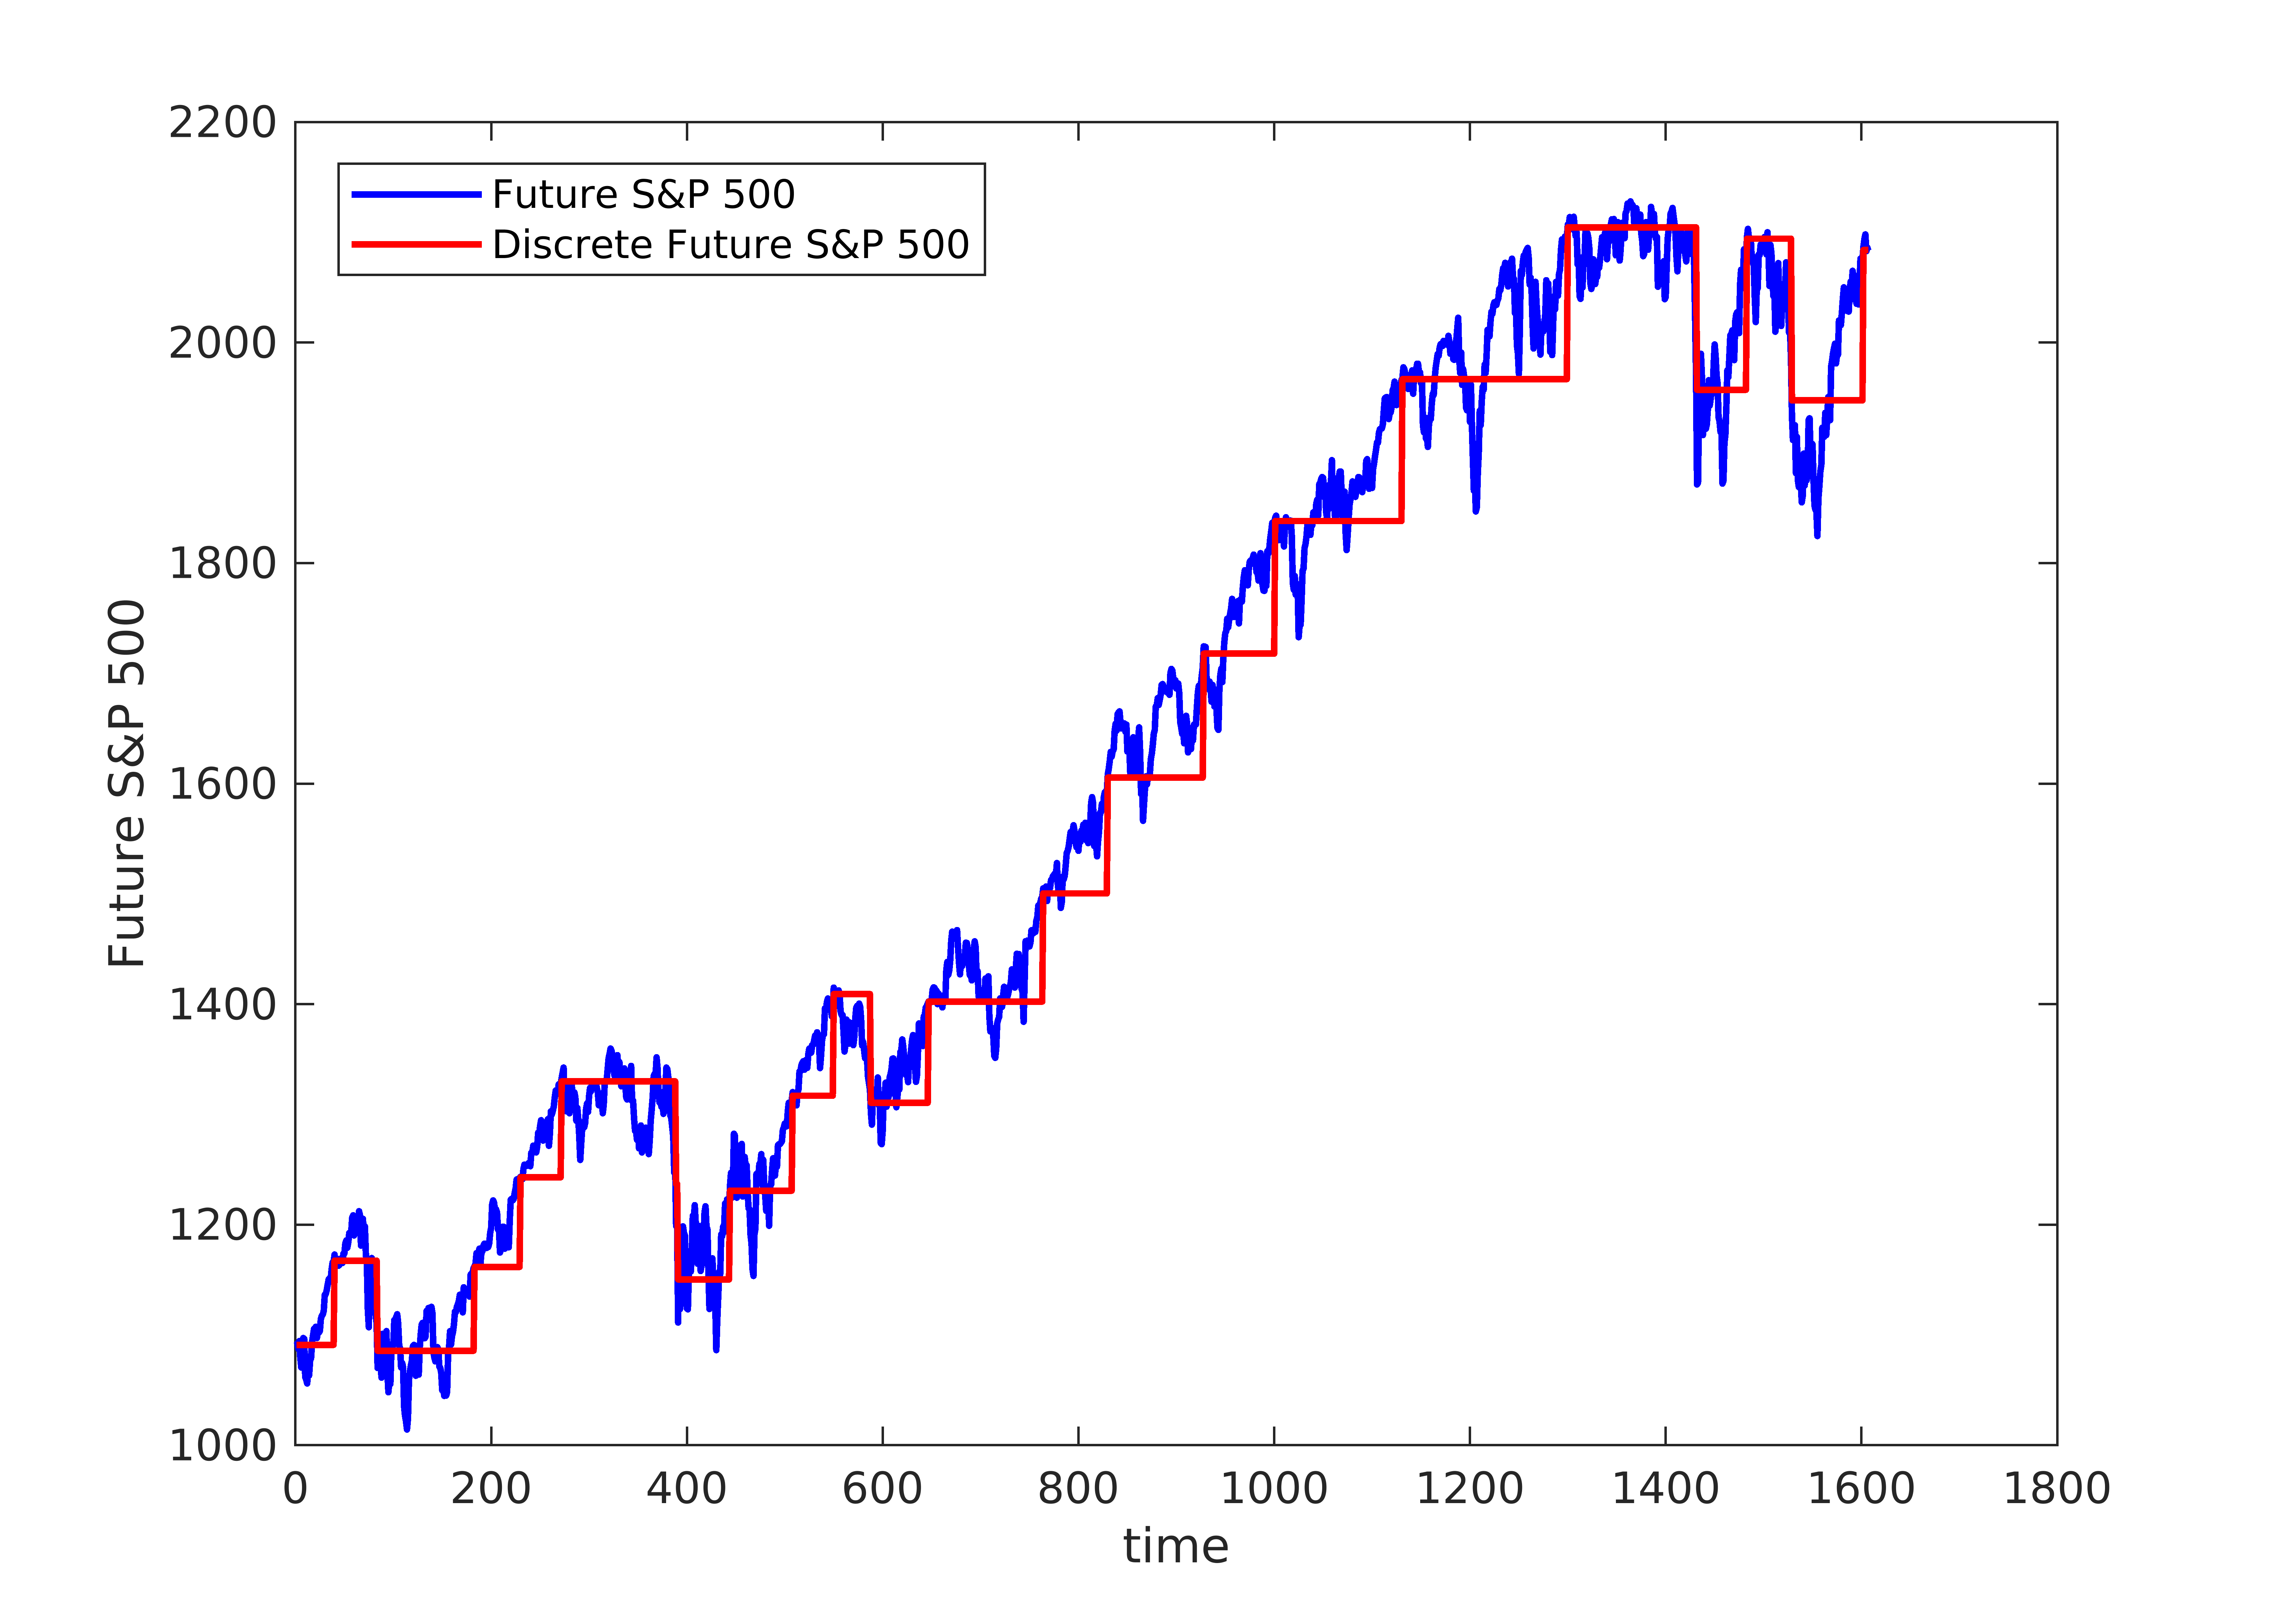
\includegraphics[scale = 0.7]{Images/DiscreteDynamics}
	\caption{Future S\&P 500 and its discrete time series. The discrete time series was obtained with a jump size $J=7\%$}
	\label{fig:DiscreteDynamics}
\end{figure}
The likelihood function can be written as follows
\begin{equation*}
\begin{split}
L(\lambda,p;\mathbf{y}) & = \prod_{i=1}^{n}f_{N^{\Delta t}_{k+1}}(y_i;\lambda,p)\\
& =\Big(\prod_{y_i = 0}\exp(-\lambda\Delta t) \Big)
\Big(\prod_{y_i=1}\big(1-\exp(-\lambda\Delta t) \big)p \Big)
\Big(\prod_{y_i=-1}\big(1-\exp(-\lambda\Delta t)\big)(1-p) \Big)\\
& = \Big(\exp(-\lambda\Delta t) \Big)^\alpha
\Big(\big(1-\exp(-\lambda\Delta t) \big)p \Big)^\beta
\Big(\big(1-\exp(-\lambda\Delta t)\big)(1-p) \Big)^\gamma
\end{split}
\end{equation*}
where 
con 
\[ \alpha =  \text{card}\{y_i = 0 \colon i = 1,\ldots,n\}\]
\[ \beta =  \text{card}\{y_i = 1 \colon i = 1,\ldots,n\}\]
\[ \gamma =  \text{card}\{y_i = -1 \colon i = 1,\ldots,n\}\]
and $\Delta t$ has been set to 1/252. Imposing the first order optimality condition $\nabla \log(L(\lambda,p;\mathbf{y}))=\bm{0}$
and solving with respect to $p$ and $\lambda$ we obtain the following estimates
\begin{align}
\widehat{\lambda} &= -\frac{1}{\Delta t}\log\Big(\frac{\alpha}{\alpha+\beta+\gamma}\Big)\\[2ex]
\widehat{p}& = \frac{\beta}{\beta+\gamma}
\end{align}
The point $(\widehat{p},\widehat{\lambda})$ is actually a maximizer since the Hessian matrix computed in this point is definite negative.
\begin{remark}
	As $\alpha+\beta+\gamma$ equals $n$ (the sample size), the estimator of $\lambda$ depends only on the number of interval in which there are no jumps ($\alpha$). Conversely, the estimator of $p$ depends only on the number of positive and negative jumps, as it was reasonable to expect.  
\end{remark}
\section{Numerical Results}
\begin{figure}
	%\centering
	\makebox[\textwidth][c]{
	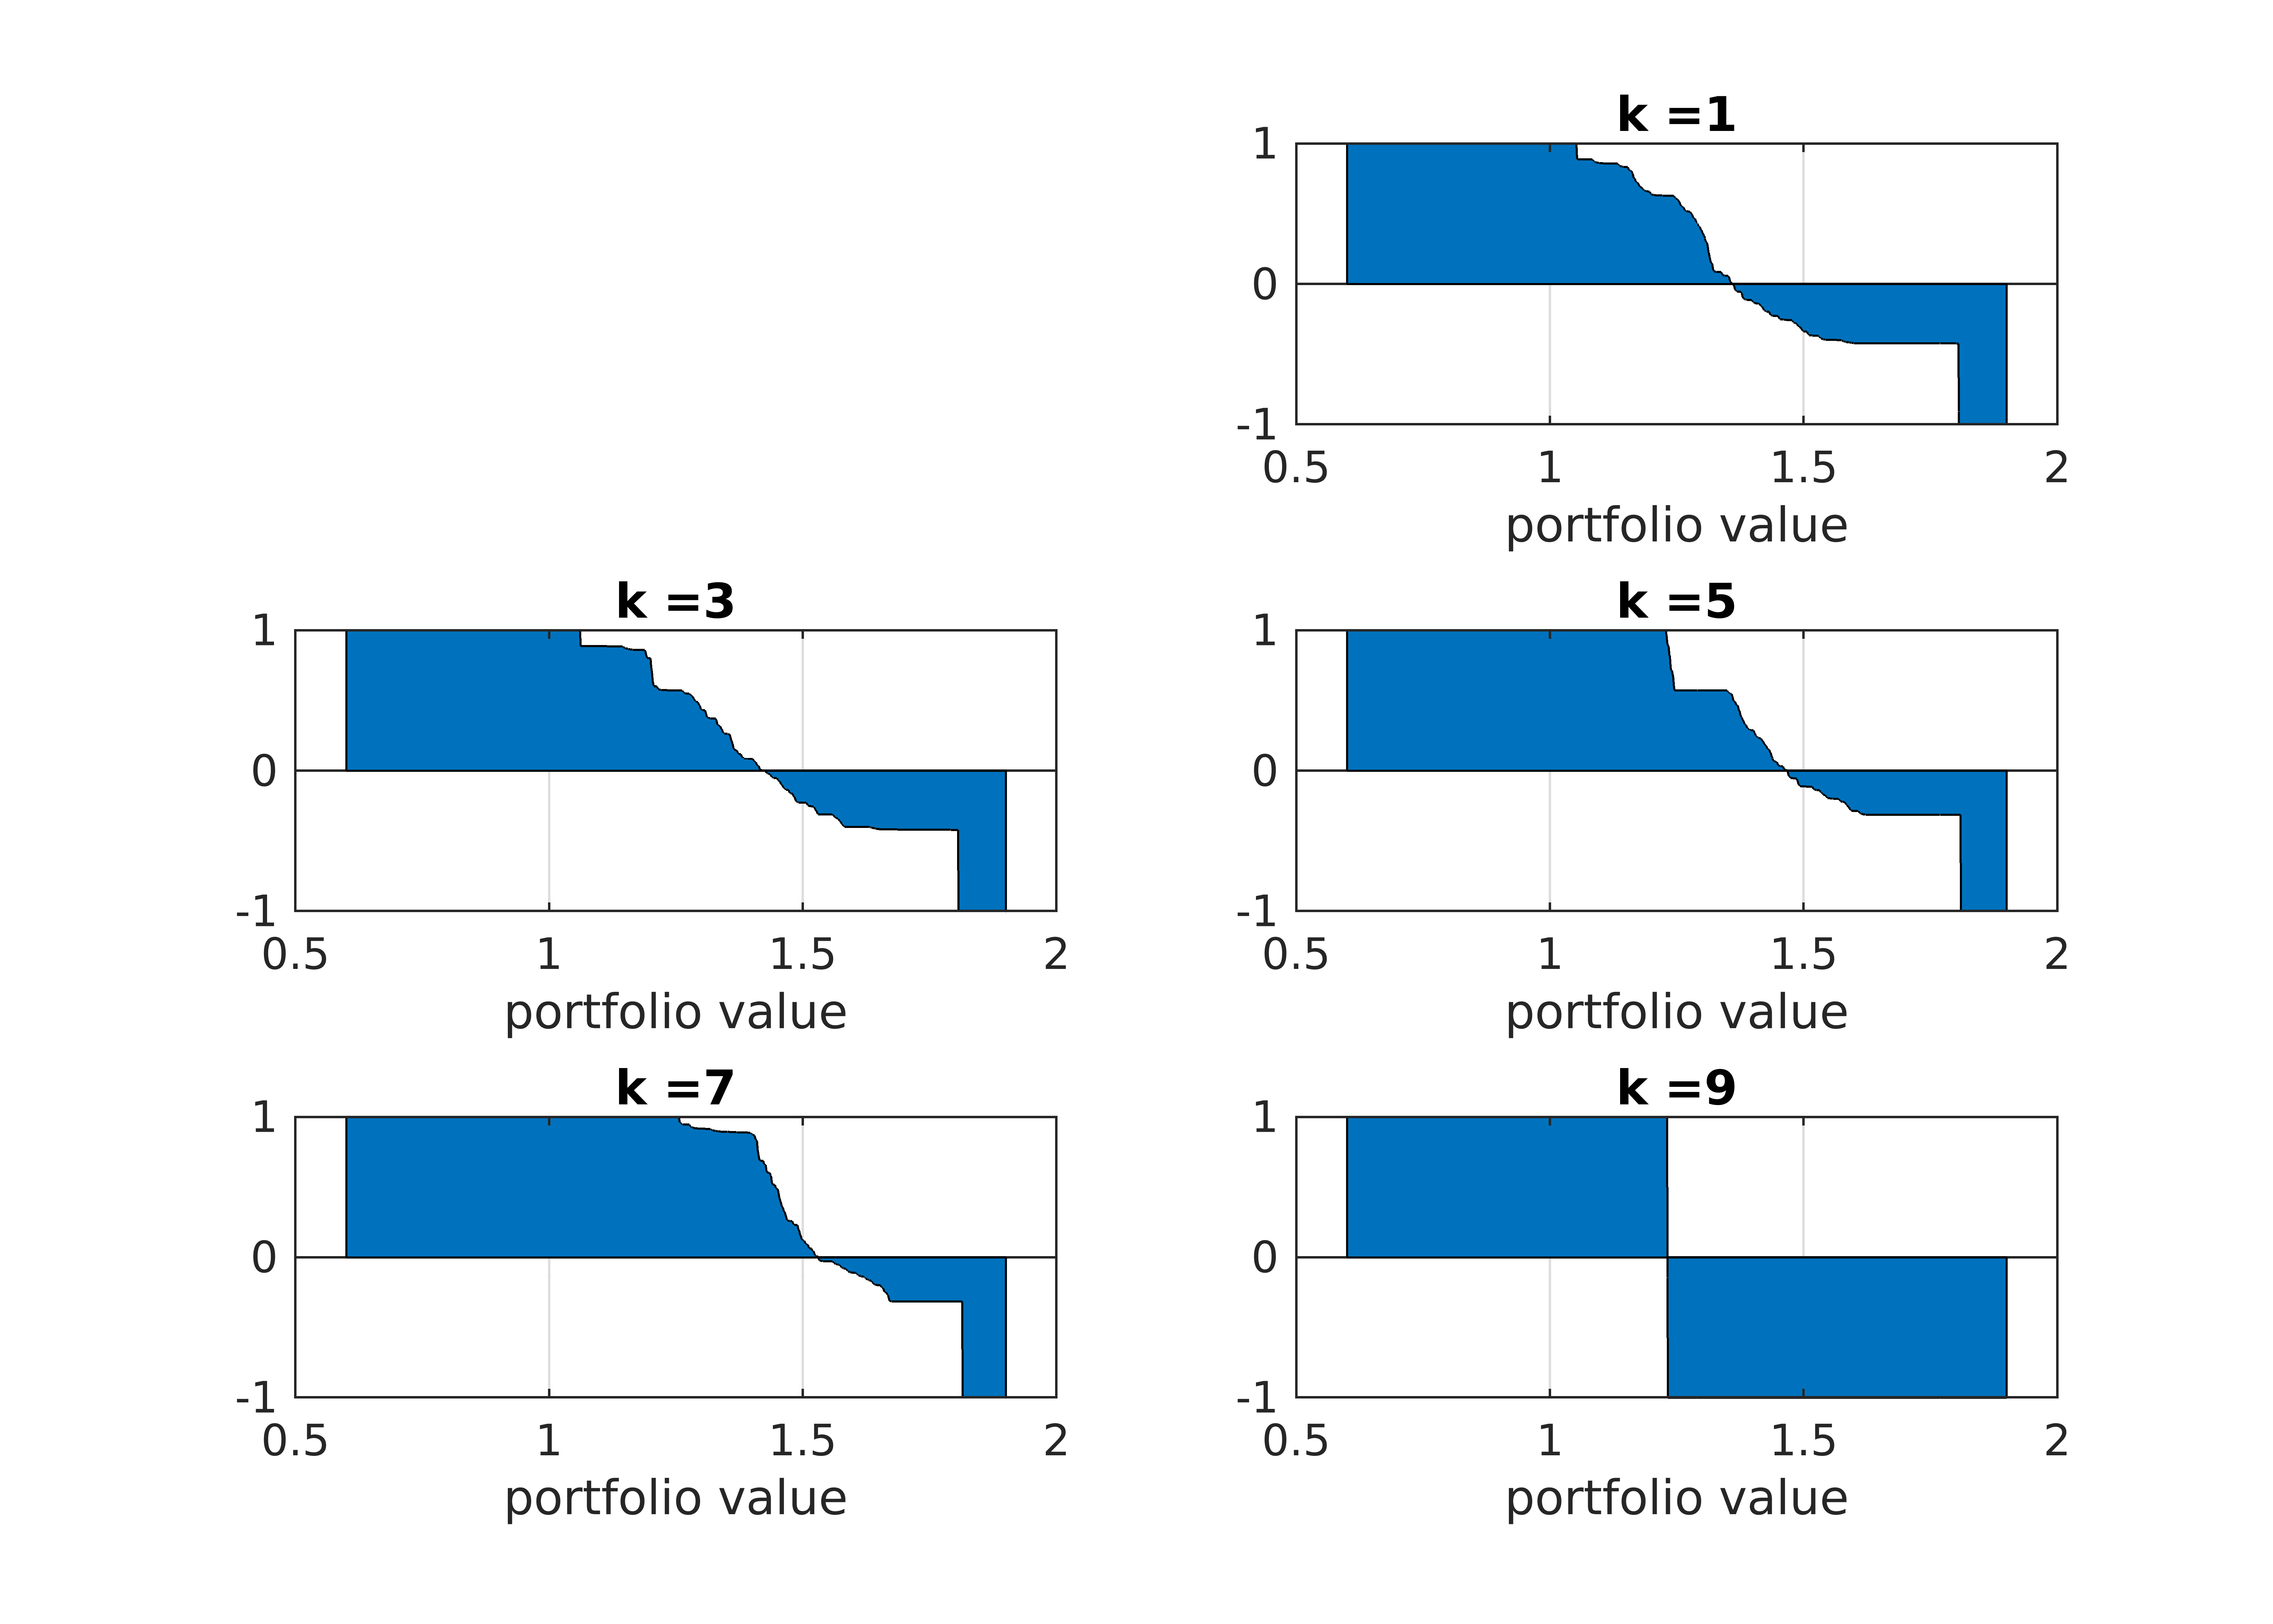
\includegraphics[scale = 0.6]{Images/mapsbasic}}
	\caption{allocation maps}
	\label{fig:basic_maps}
\end{figure}




\chapter{Model Extensions}\label{chpt:Model_Extensions}
The prime objective of this chapter is to extend the event-driven model of Chapter \ref{chpt:ED} in two different ways. On one hand, in Section \ref{sec:GBM} the risky asset will be modeled in continuous-time as a \gls{GBM}, on the other hand, in Section \ref{sec:Interest_rate_dynamics} we no longer let the risk-free asset evolve deterministically but instead its short-rate will evolve according to the Vasicek model. 
\section{A GBM dynamics for the risky asset}\label{sec:GBM}
Let us consider the same portfolio as the one in Chapter \ref{chpt:ED}, namely a risky and a risk-free asset. As far as the risk-free asset is concerned, the deterministic model of Chapter \ref{chpt:ED} remains unchanged. On the other hand, the following dynamics for the risky asset is assumed
\begin{equation}\label{eq:GBM_SDE}
\begin{cases*}
dS_t  = \mu S_t dt + \sigma S_t dW_t\\
S_{t_k} = S_k, \quad t\geq t_k
\end{cases*}
\end{equation}
where $\{W_t\}_{t\geq t_k}$ is a unidimensional Brownian motion, $\mu \in \mathbb{R}$, $\sigma > 0$ and $t_k$ is the time when the $k$th event occurs. Solving the above \gls{SDE} brings 
\begin{align*}
S_t & = S_k \exp\big\{(\mu-\sigma^2/2)(t-t_k)+\sigma(W_t-W_{t_k})\}\\
& = S_k \exp\big\{\widetilde{\mu}(t-t_k)+\sigma(W_t-W_{t_k})\}
\end{align*}
where we defined $\widetilde{\mu}= \mu-\sigma^2/2$. The cumulative risky asset log-return (starting from $t_k$) is denoted by $\{X_t\}_{t\geq t_k}$ and is equal to
\begin{equation}
X_t = \log\big(S_t/S_{t_k}\big)=\widetilde{\mu}(t-t_k) + \sigma(W_t-W_{t_k}).
\end{equation}
Given that in the development of the model it will be more convenient to have the time starting from 0, exploiting the Translation Invariance property of Brownian motion we define the translated log-return process as follows
\begin{equation}\label{eq:translatedGBM}
\widetilde{X}_t = X_{t+t_k} = \widetilde{\mu}t + \sigma(W_{t+t_k}-W_{t_k}) = \widetilde{\mu}t + \sigma \widetilde{W}_t \quad t\geq 0.
\end{equation}
In this case $t$ represents the interevent time instead of clock time.
\subsection{The double exit problem }
In the event-driven setting introduced in the previous chapter, what triggers a portfolio rebalancing is the fact that the absolute value of process $\widetilde{X}_t$ exceeds the barrier $J$. When this happens, we say, in the event-driven jargon, that an event has occurred. Therefore, it is of prime interest  modeling the stochastic time instant in which the next event takes place. This could be done by defining the following stopping time
\begin{align}\label{eq:stopping_time}
\tau_{k+1} & = \inf\big\{t\geq 0 \colon \lvert\widetilde{X}_t\lvert\geq J \big\}\\\nonumber
& = \inf\big\{t\geq 0 \colon \widetilde{X}_t \notin (-J,J) \big\}.
\end{align}
Given that the density function of $x_{k+1}$ is needed in the \gls{ODAA} algorithm, we are interested in the distribution of random variable (\ref{eq:stopping_time}). This problem is known in literature as \textit{the double exit problem of a Brownian motion with drift}. The central result is given by the following theorem, which covers a more general case in which the upper and lower barrier are different. The theorem is taken from \cite{Hieber2012} as is.
\begin{theorem}[double exit problem]\label{thm:double_exit_problem}
	Let $X_t = \mu t + \sigma W_t$ be a Brownian motion with drift, $\mu \in \mathbb{R}$ and $\sigma > 0$. Moreover, assume there are two constant barriers $b<0<a$. The distribution of $\tau = \inf\big\{t\geq 0 \colon X_t \notin (b,a) \big\}$ is 
	\[
	F_{\tau}(t) = 1-\bigg(\exp\Big\{\frac{\mu b}{\sigma^2}\Big\}K_t^{\infty}(a)-\exp\Big\{\frac{\mu a}{\sigma^2}\Big\}K_t^{\infty}(b) \bigg)
	\]
	where
	\[
	K_t^N(k)= \frac{\sigma^2\pi}{(a-b)^2}\sum_{n=1}^{N}\frac{n(-1)^{n+1}}{\frac{\mu^2}{2\sigma^2}+\frac{\sigma^2n^2\pi^2}{2(a-b)^2}}\exp\bigg\{-\bigg(\frac{\mu^2}{2\sigma^2}+\frac{\sigma^2n^2\pi^2}{2(a-b)^2}\bigg)t\bigg\}\sin\Big(\frac{n\pi k}{a-b}\Big).
	\]
	Applying the theorem to our case ($a=J, b=-J$) we get 
	\begin{equation}\label{eq:cdf_ext1}
	F_{\tau_{k+1}}(t)=1-\bigg[2\cosh\Big(\frac{\widetilde{\mu}J}{\sigma^2}\Big)K_t^{\infty}(J)\bigg],
	\end{equation}
	where we used the fact that $K_t^N(k)$ is odd as a function of $k$.
\end{theorem}

\begin{remark}
	Theorem \ref{thm:double_exit_problem} does not assume the upper and lower barrier to be equal. This generality would allow us to consider a more realistic case in which a portfolio riallocation is triggered, for example, when the cumulative return process is grater than a barrier $J_{up}$ or lower than $-J_{down}$, where $J_{up} > J_{down}$.
\end{remark}
\subsection{Portfolio dynamics and the density of $x_{k+1}$}
Following the same path as in Chapter \ref{chpt:ED}, we are left to compute the event-driven portfolio dynamics and the portfolio value density function. As far as the first issue is concerned, the dynamics can be written as follows
\begin{equation}\label{eq:GBM_portfolio_dynamics}
\boxed{x_{k+1}=x_k\big(\exp\{r\tau_{k+1}\} + u_k\widetilde{X}_{\tau_{k+1}}\big)} \qquad k \in \mathbb{N}
\end{equation}
where $r$ is the constant risk-free asset return, $\tau_{k+1}$ is the stopping time (\ref{eq:stopping_time}), $u_k$ is the risky asset portfolio weight and $\widetilde{X}_{\tau_{k+1}}$ is the return process computed at the random time $\tau_{k+1}$. $\widetilde{X}_{\tau_{k+1}}$ can only assume value $J$ or $-J$, therefore it is a Bernoullian random variable. The value of its parameter $p$ is given in the following lemma (which closely follows exercise 5.20, \cite{baldi2017})
\begin{lemma}\label{lemma:probability_positive_jump}
	Let $\widetilde{X}_t$ be the return process (\ref{eq:translatedGBM}) and $\tau_{k+1}$ the stopping time (\ref{eq:stopping_time}). Then $\widetilde{X}_{\tau_{k+1}} \sim B(p)$ where 
	\begin{align}
	p &= \mathbb{P}\Big(\widetilde{X}_{\tau_{k+1}}=J\Big)\\[2ex]\nonumber
	&=\frac{1-\exp\{2\widetilde{\mu}J/\sigma^2\}}{\exp\{-2\widetilde{\mu}J/\sigma^2\} - \exp\{2\widetilde{\mu}J/\sigma^2\}} \\[2ex]\nonumber
	& = \frac{\exp\{2\widetilde{\mu}J/\sigma^2\}-1}{2\sinh(2\widetilde{\mu}J/\sigma^2)}.
	\end{align}
\end{lemma}
\begin{proof}
	The first step of the proof consists in finding $\xi \in \mathbb{R}\setminus\{0\}$ such that $M=\exp\{\xi \widetilde{X}_t\}$ is a martingale. To this end, we apply Ito's formula (\cite{baldi2017}, Theorem 8.1) to $M_t$:
	\begin{align}\label{eq:Mt_dynamics}
	\nonumber
	dM_t & = \xi M_t d\widetilde{X}_t+\frac{1}{2}\xi^2M_t\sigma^2dt\\
	     & = \Big(\widetilde{\mu}\xi + \frac{1}{2}\sigma^2\xi^2\Big)M_t dt + \sigma\xi M_t d\widetilde{W}_t.
	\end{align}
	If the drift in (\ref{eq:Mt_dynamics}) is null then $\{M_t\}_{t\geq0}$ is a martingale. Therefore, we impose the condition $\widetilde{\mu}\xi + \frac{1}{2}\sigma^2\xi^2 = 0$ which brings $ \xi = -2\widetilde{\mu}/\sigma^2$.
	
	The second part of the proof starts by noticing that also the process $\{M_{t\wedge\tau}\}_{t\geq 0}$ is a martingale\footnote{for the sake of clarity, we dropped the subscript $k+1$ from $\tau_{k+1}$}(Proposition 5.6, \cite{baldi2017}). Moreover, since $\lvert M_{t\wedge\tau} \lvert \leq J$ for every $t\geq0$, we can apply the Dominated Convergence Theorem (Proposition 4.2, \cite{baldi2017}) in the following way:
	\begin{align*}
	\mathbb{E}\big[M_{\tau}\big] & = \mathbb{E}\Big[\lim\limits_{t\to\infty}M_{t\wedge\tau}\Big] = & (\text{Dominated Conv. Theorem})\\[2ex]
	& = \lim\limits_{t\to\infty}\underbrace{\mathbb{E}\big[M_{t\wedge\tau}\big]}_{1}=\\
	& = 1
	\end{align*}
	hence
	\begin{align*}
	\mathbb{E}\big[M_{\tau}\big] & = \exp\{2\widetilde{\mu}J/\sigma^2\}\mathbb{P}\Big(\widetilde{X}_{\tau}=-J\Big) + \exp\{-2\widetilde{\mu}J/\sigma^2\}\mathbb{P}\Big(\widetilde{X}_{\tau}=J\Big) \\[2ex]
	& = \exp\{2\widetilde{\mu}J/\sigma^2\}\bigg(1-\underbrace{\mathbb{P}\Big(\widetilde{X}_{\tau}=J\Big)}_{p}\bigg) + \exp\{-2\widetilde{\mu}J/\sigma^2\}\underbrace{\mathbb{P}\Big(\widetilde{X}_{\tau}=J\Big)}_{p} \\
	& = 1.
	\end{align*}
	Finally, solving for $p$ we obtain the result.
\end{proof}

In order to apply the \gls{ODAA} algorithm we need the probability density function of random variable $x_{k+1}$. Its explicit form is given in the following proposition.
\begin{proposition}
	Let $x_{k+1}$ be the random variable (\ref{eq:GBM_portfolio_dynamics}) (where $x_k$ has been fixed to $x \in \mathcal{X}$). Its density function is
	\begin{equation}\label{eq:DensityGBM}
	f_{x_{k+1}}(z) = \frac{2\cosh\big(\frac{\tilde{\mu}J}{\sigma^2}\big)}{rx}\Big[p \Gamma^\infty_{\frac{z-\xi}{x}}(J) \mathbbm{1}_{(x+\xi,\infty)} + (1-p)\Gamma^\infty_{\frac{z+\xi}{x}}(J) \mathbbm{1}_{(x-\xi,\infty)}  \Big]
	\end{equation}
	where $\xi = xu_kJ$, $p$ is the probability given by Lemma \ref{lemma:probability_positive_jump} and
	\begin{equation}\label{eq:Gamma}
	\Gamma^\infty_{z}(J) =\frac{\sigma^2\pi}{4J^2}\sum_{n=1}^{\infty}n(-1)^{n+1}z^{-\frac{1}{r}\big(\frac{\tilde{\mu}^2}{2\sigma^2} + \frac{\sigma^2n^2\pi^2}{8J^2}\big)-1}\sin(\frac{\pi}{2}n)
	\end{equation}
\end{proposition}
\begin{proof}
	The scheme of the proof is the same as the one in Proposition \ref{prop:density_portfolio_basic}. Let us rewriting the portfolio dynamics as 
	\[ x_{k+1}=x\exp\{r\tau_{k+1}\}+xu_k\widetilde{X}_{\tau_{k+1}}=Y+xu_k\widetilde{X}_{\tau_{k+1}}. \]
	The first step is to find the cdf of $Y$.Thanks to Theorem \ref{thm:double_exit_problem} we have
	\begin{align*}
	F_Y(y) & =\mathbb{P}\Big(x\exp\{r\tau_{k+1}\}\leq y\Big)= F_{\tau_{k+1}}\Big(\frac{1}{r}\log\big(y/x\big)\Big) \\[2ex]
	& = \bigg\{ 1-\Big[2\cosh(\widetilde{\mu}J/\sigma^2)K_{\frac{1}{r}\log(\frac{y}{x})}^{\infty}(J)  \Big]\bigg\}\mathbbm{1}_{[x,\infty)}.
	\end{align*}
	By invoking the Law of Total Probability we can write
	\begin{align*}
	F_{x_{k+1}}(z) & = \mathbb{P}\big(x_{k+1}\leq z\big) \\[2ex]
	& = \mathbb{P}\Big(Y\leq z-xu_k\widetilde{X}_{\tau_{k+1}}\lvert\widetilde{X}_{\tau_{k+1}}=J\Big)\mathbb{P}\Big(\widetilde{X}_{\tau_{k+1}}=J\Big)+\\
	&\qquad + 
	\mathbb{P}\Big(Y\leq z-xu_k\widetilde{X}_{\tau_{k+1}}\lvert\widetilde{X}_{\tau_{k+1}}=-J\Big)\mathbb{P}\Big(\widetilde{X}_{\tau_{k+1}}=-J\Big)\\[2ex]
	& = F_Y(z-\xi)p + F_Y(z+\xi)(1-p)\\[2ex]
	& = p\bigg\{ 1-\Big[2\cosh(\widetilde{\mu}J/\sigma^2)K_{\frac{1}{r}\log(\frac{z-\xi}{x})}^{\infty}(J)\Big]\bigg\}\mathbbm{1}_{[x+\xi,\infty)}+\\
	& \qquad + (1-p)\bigg\{ 1-\Big[2\cosh(\widetilde{\mu}J/\sigma^2)K_{\frac{1}{r}\log(\frac{z+\xi}{x})}^{\infty}(J)\Big]\bigg\}\mathbbm{1}_{[x-\xi,\infty)}.
	\end{align*}
	where $\xi = xu_kJ$. Now, the density is obtained differentiating the cdf above. This amounts to compute $\frac{d}{dz}K_{\frac{1}{r}\log(\frac{z-\xi}{x})}^{\infty}(J)$ and $\frac{d}{dz}K_{\frac{1}{r}\log(\frac{z+\xi}{x})}^{\infty}(J)$. As an example, let us compute the first derivative:
	\begin{align*}
	\frac{d}{dz}K_{\frac{1}{r}\log(\frac{z-\xi}{x})}^{\infty}(J) & = \frac{d}{dz}\bigg(\frac{\sigma^2\pi}{4J^2}\sum_{n=1}^{\infty}\frac{n(-1)^{n+1}}{\frac{\tilde{\mu}^2}{2\sigma^2} + \frac{\sigma^2n^2\pi^2}{8J^2}}\Big(\frac{z-\xi}{x}\Big)^{-\frac{1}{r}\big(\frac{\tilde{\mu}^2}{2\sigma^2} + \frac{\sigma^2n^2\pi^2}{8J^2}\big)}\sin\big(\frac{\pi}{2}n\big)  \bigg)\\[2ex]
	& = \big(-\frac{1}{rx}\big)\frac{\sigma^2\pi}{4J^2}\sum_{n=1}^{\infty}n(-1)^{n+1} \Big(\frac{z-\xi}{x}\Big)^{-\frac{1}{r}\big(\frac{\tilde{\mu}^2}{2\sigma^2} + \frac{\sigma^2n^2\pi^2}{8J^2}\big)-1}\sin\big(\frac{\pi}{2}n\big)\\[2ex]
	& = \big(-\frac{1}{rx}\big)\Gamma_{\frac{z-\xi}{x}}^{\infty}(J).
	\end{align*}
	Substituting into
	\[
	f_{x_{k+1}}(z) =2\cosh\Big(\frac{\widetilde{\mu}J}{\sigma^2}\Big)\Big[-p\frac{d}{dz}K_{\frac{1}{r}\log(\frac{z-\xi}{x})}^{\infty}(J)\mathbbm{1}_{(x+\xi,\infty)}-(1-p)\frac{d}{dz}K_{\frac{1}{r}\log(\frac{z+\xi}{x})}^{\infty}(J)\mathbbm{1}_{(x-\xi,\infty)}\Big]
	\]
	and rearranging, gives us the result.
\end{proof}
Density (\ref{eq:DensityGBM}) is plotted in Figure \ref{fig:PtfDensity} for different values of the risky asset portfolio weight $u_k$.
\begin{figure}[]
	%\centering
	\makebox[\textwidth][c]{
		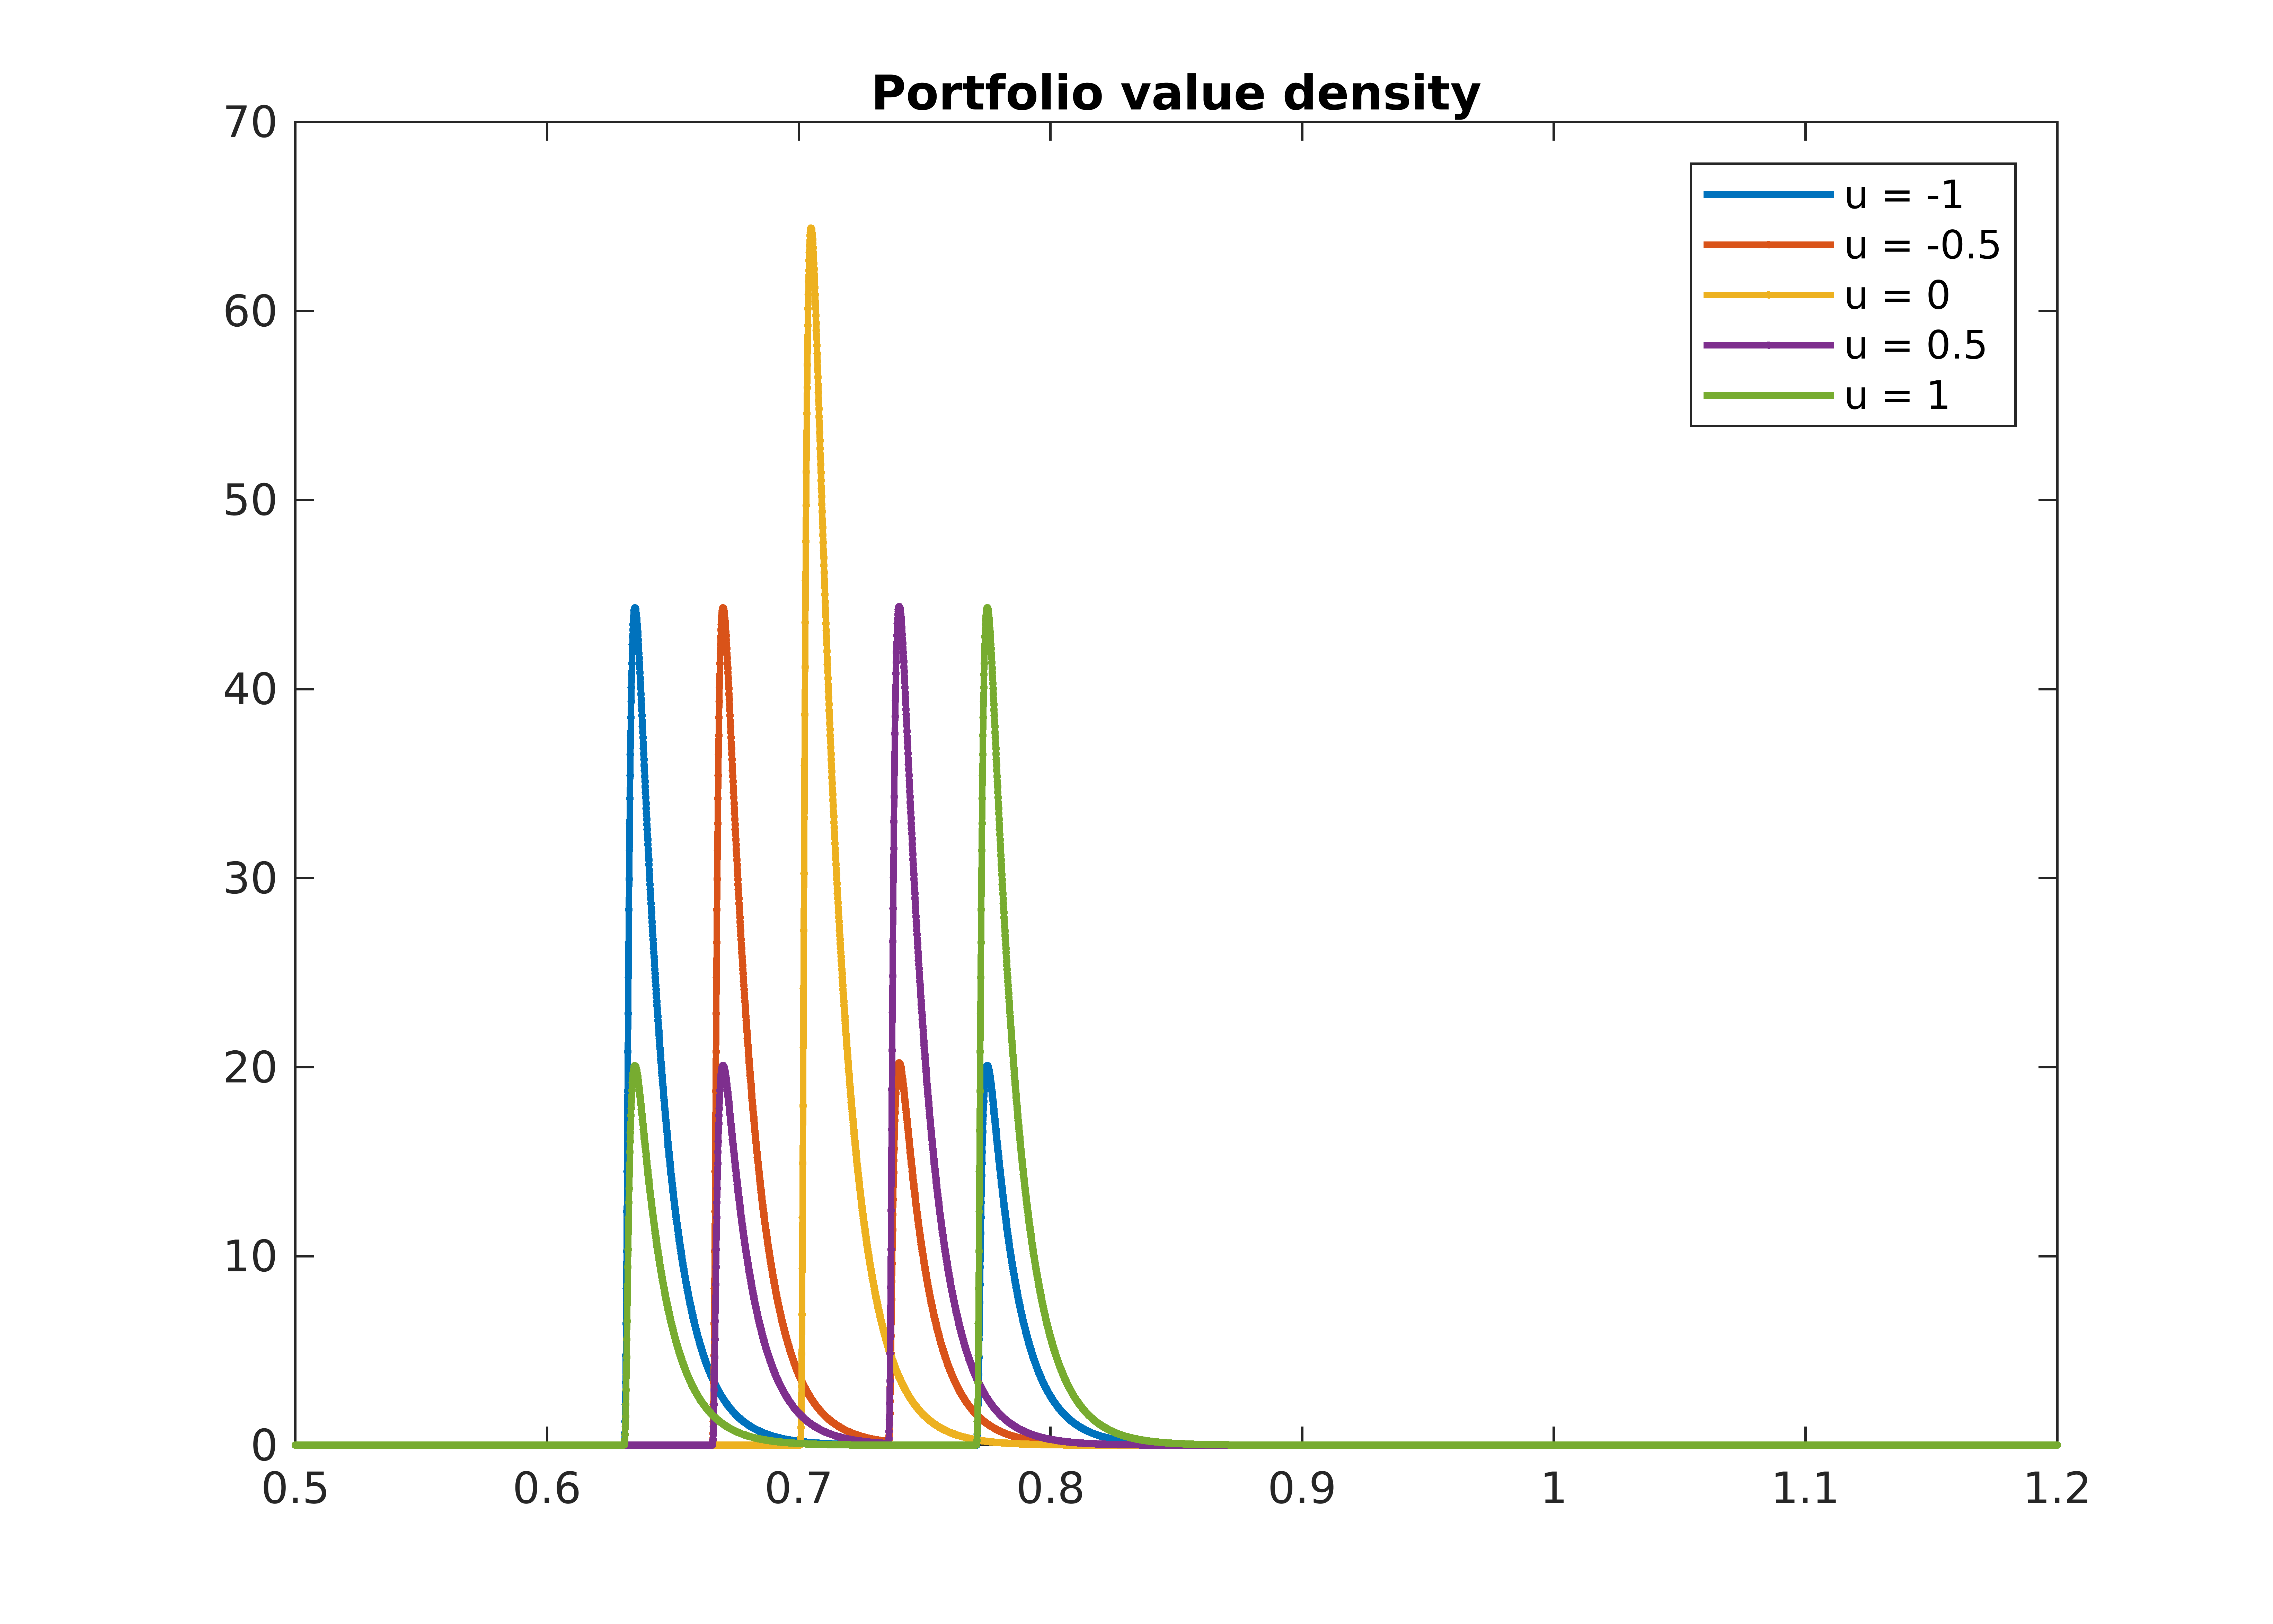
\includegraphics[scale = 0.5]{Images/PtfDensity}}
	\caption{Probability density function of random variable variable $x_{k+1}$ for different value of the risky-asset weight $u_k$ and the following parameters: $x=0.7$, $r=5.5\%$, $\mu=0.114$, $\sigma=0.1602$ and $J=10\%$}
	\label{fig:PtfDensity}
\end{figure}

\subsection{Numerical results}
In this section we report the results obtained by applying the \gls{ODAA} algorithm in an event-driven framework and modeling the risky asset as a Geometric Brownian Motion. Before showing the results however, we need to discuss the calibration of parameter $\mu$ and $\sigma$ of the \gls{GBM} dynamics to market data and the truncation of the series in (\ref{eq:Gamma}). As far as data is concerned, we use the same time series presented in Section \ref{sec:ED_dataset} (observations from the Future S\&P 500 index from 22 January 2010 to 25 April 2016).
\paragraph{\gls{GBM} calibration}
Let us consider the discretized solution of \gls{SDE} (\ref{eq:GBM_SDE})
\begin{align*}
S_{t_{k+1}} & = S_{t_k}\exp\big\{(\mu-\frac{1}{2}\sigma^2)\Delta t+\sigma(W_{t_{k+1}}-W_{t_k})\big\} \\
& = S_{t_k}\exp\big\{(\mu-\frac{1}{2}\sigma^2)\Delta t+\sigma\sqrt{\Delta t}Z\big\}
\end{align*}
where $Z \sim \mathcal{N}(0,1)$. In terms of log-return, we have
\[X_{t_{k+1}} = (\mu-\frac{1}{2}\sigma^2)\Delta t+\sigma\sqrt{\Delta t}Z.\] 
Let $x_1,\ldots,x_n$ be a random sample of log-returns from a normal population with mean $(\mu-\frac{1}{2}\sigma^2)\Delta t$ and variance $\sigma^2 \Delta t$. From this random sample we obtain the following estimates
\begin{align*}
\widehat{\sigma}^2 & = \frac{s^2}{\Delta t}\\[1.5ex]
\widehat{\mu} & = \frac{\bar{x}}{\Delta t} + \frac{1}{2}\widehat{\sigma}^2
\end{align*}
where $s^2$ is the sample variance and $\bar{x}$ the sample mean. Setting $\Delta t = 1/252$ and applying the equations above to our data we get $\widehat{\mu} = 0.1143$ and $\widehat{\sigma} = 0.1602$.


\paragraph{Series truncation}
In practice, the series in (\ref{eq:Gamma}) has to be truncated. Let $\Gamma^N_z(J)$ be the function in (\ref{eq:Gamma}) when the series is truncated at the $N$th term. The residual could be bounded in the following way
\begin{align*}
\big\lvert\Gamma^{\infty}_z(J)-\Gamma^N_z(J)\big\lvert & \leq \frac{\sigma^2\pi}{4J^2}\bigg\lvert\sum_{n=N+1}^{\infty}n(-1)^{n+1}z^{-\frac{1}{r}\big(\frac{\tilde{\mu}^2}{2\sigma^2} + \frac{\sigma^2n^2\pi^2}{8J^2}\big)-1}\sin(\frac{\pi}{2}n)\bigg\lvert\\
& \leq \frac{\sigma^2\pi}{4J^2} \sum_{n=N+1}^{\infty}nz^{-\frac{1}{r}\big(\frac{\tilde{\mu}^2}{2\sigma^2} + \frac{\sigma^2n^2\pi^2}{8J^2}\big)-1}\\
& \leq \frac{\sigma^2\pi}{4J^2} \int_{N}^{\infty}nz^{-\frac{1}{r}\big(\frac{\tilde{\mu}^2}{2\sigma^2} + \frac{\sigma^2n^2\pi^2}{8J^2}\big)-1}\mathrm{d}n\\
& \leq \frac{r}{\pi \log z}z^{-\frac{1}{r}\big(\frac{\tilde{\mu}^2}{2\sigma^2} + \frac{\sigma^2N^2\pi^2}{8J^2}\big)-1}
\end{align*}
therefore, denoting by $\epsilon$ the maximum error tolerance, we obtain
\begin{equation}
N(z) \geq \sqrt{-\frac{8rJ^2}{\sigma^2\pi^2}\bigg\{\frac{\widetilde{\mu}^2}{2r\sigma^2}+\log_z\Big(\frac{\epsilon\pi z \log z}{r}\Big) \bigg\}}.
\end{equation}
which is the minimum number of terms in the series in order to have the specified accuracy.

We considered an investment characterized by the following parameters:
\begin{itemize}
	\item Initial wealth $x_0 = 1$.
	\item $J = 10\%$.
	\item $N = 10$ portfolio rebalancings.
	\item The following target sets: $X_0 = \{1\}$, $X_k = [0,\infty)$ for $k = 1,\ldots,9$ and $X_{10} = [(1+\theta)^3,\infty)$  with $\theta=7\%$. In the implementation, they were approximated by $X_k = [0.7,2]$ for $k = 1,\ldots,9$ and $X_{10} = [(1+\theta)^3,2]$ and discretized with a step length of $2 \times 10^{-4}$.
	\item $r = 1\%$ (risk-free rate of return).
\end{itemize}
The allocation maps obtained via \gls{ODAA} algorithm exhibit the \textit{contatrian} attitude typical of all the \gls{ODAA} strategies presented so far. The joint probability of reaching the target sets is $p^{\star}=J(x_0) = 0.8834$. This result is verified by running a Monte Carlo simulation with $2\times10^6$ replications at each rebalancing period. The outcome in terms of joint probability and other investment statistics, is reported in Table \ref{tab:performance_ext1}. Finally, in Figure \ref{fig:ext1_investment_return} we show the empirical density function of the annualized investment return.




%\begin{figure}[]
%	%\centering
%	\makebox[\textwidth][c]{
%		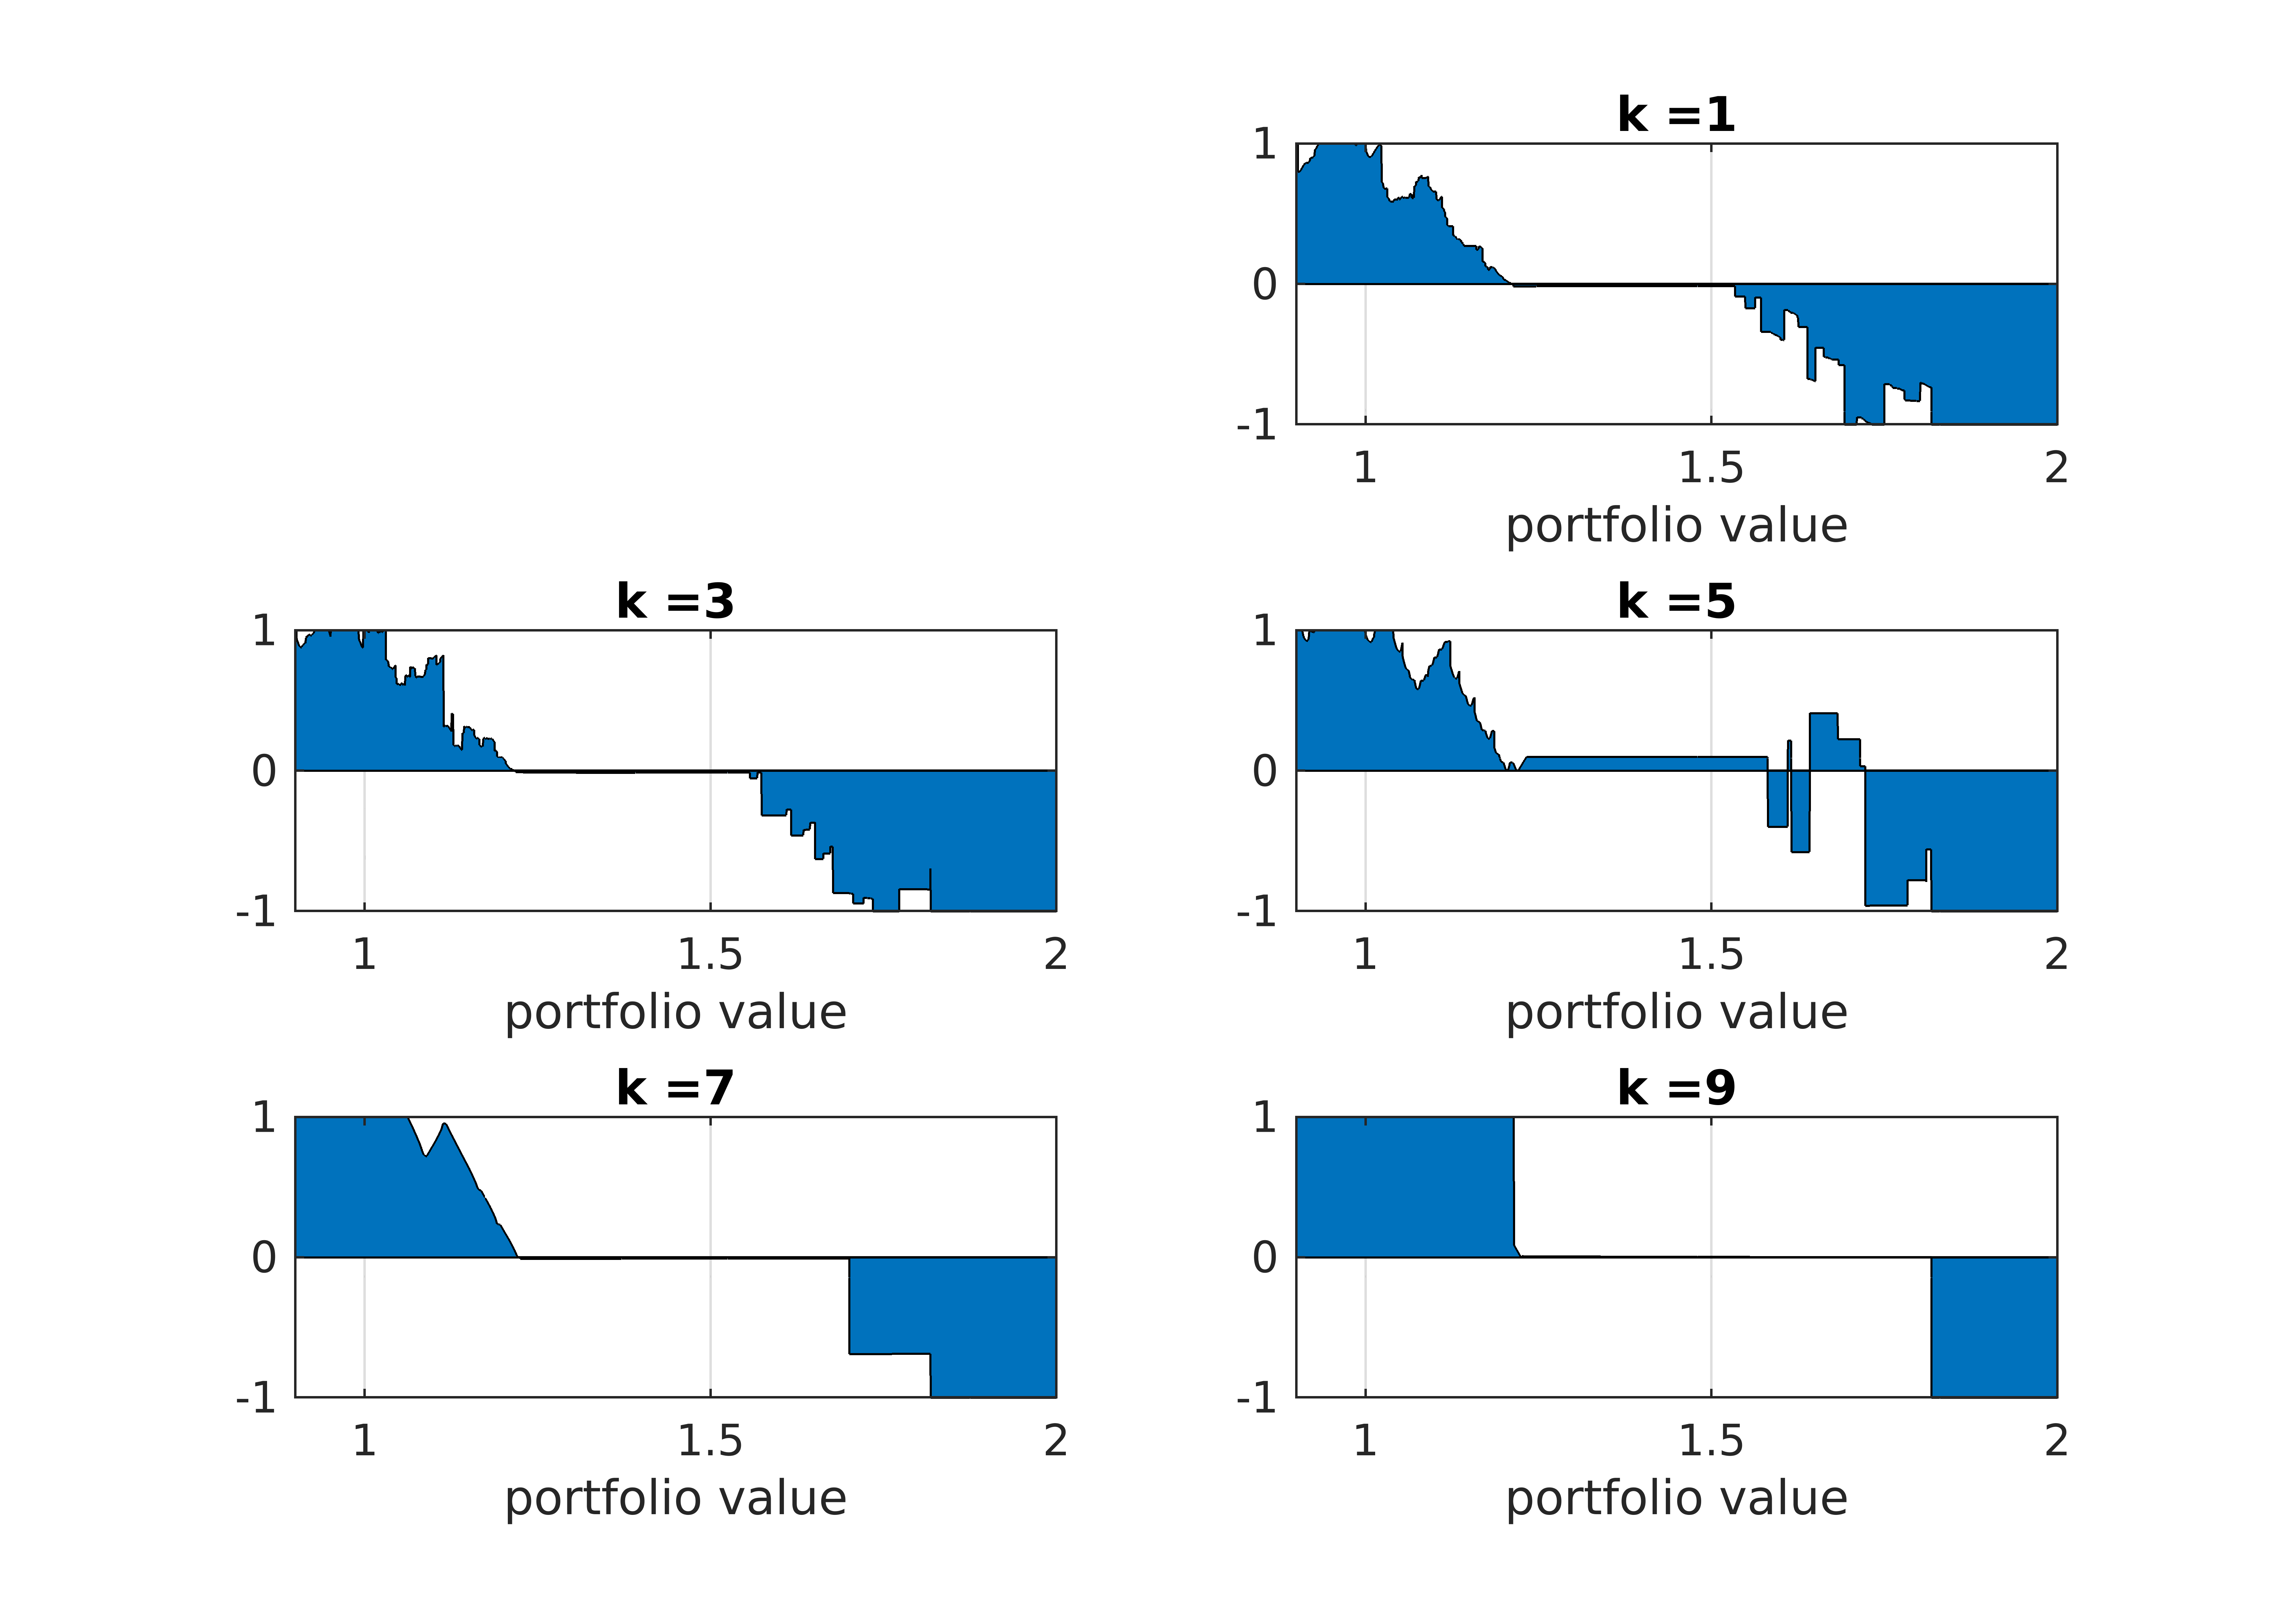
\includegraphics[scale = 0.8]{Images/mapsext1}}
%	\caption{allocation maps for the risky asset, which is modeled according to a Geometric Brownian Motion }
%	\label{fig:ext1_maps}
%\end{figure}


\begin{figure}[]
	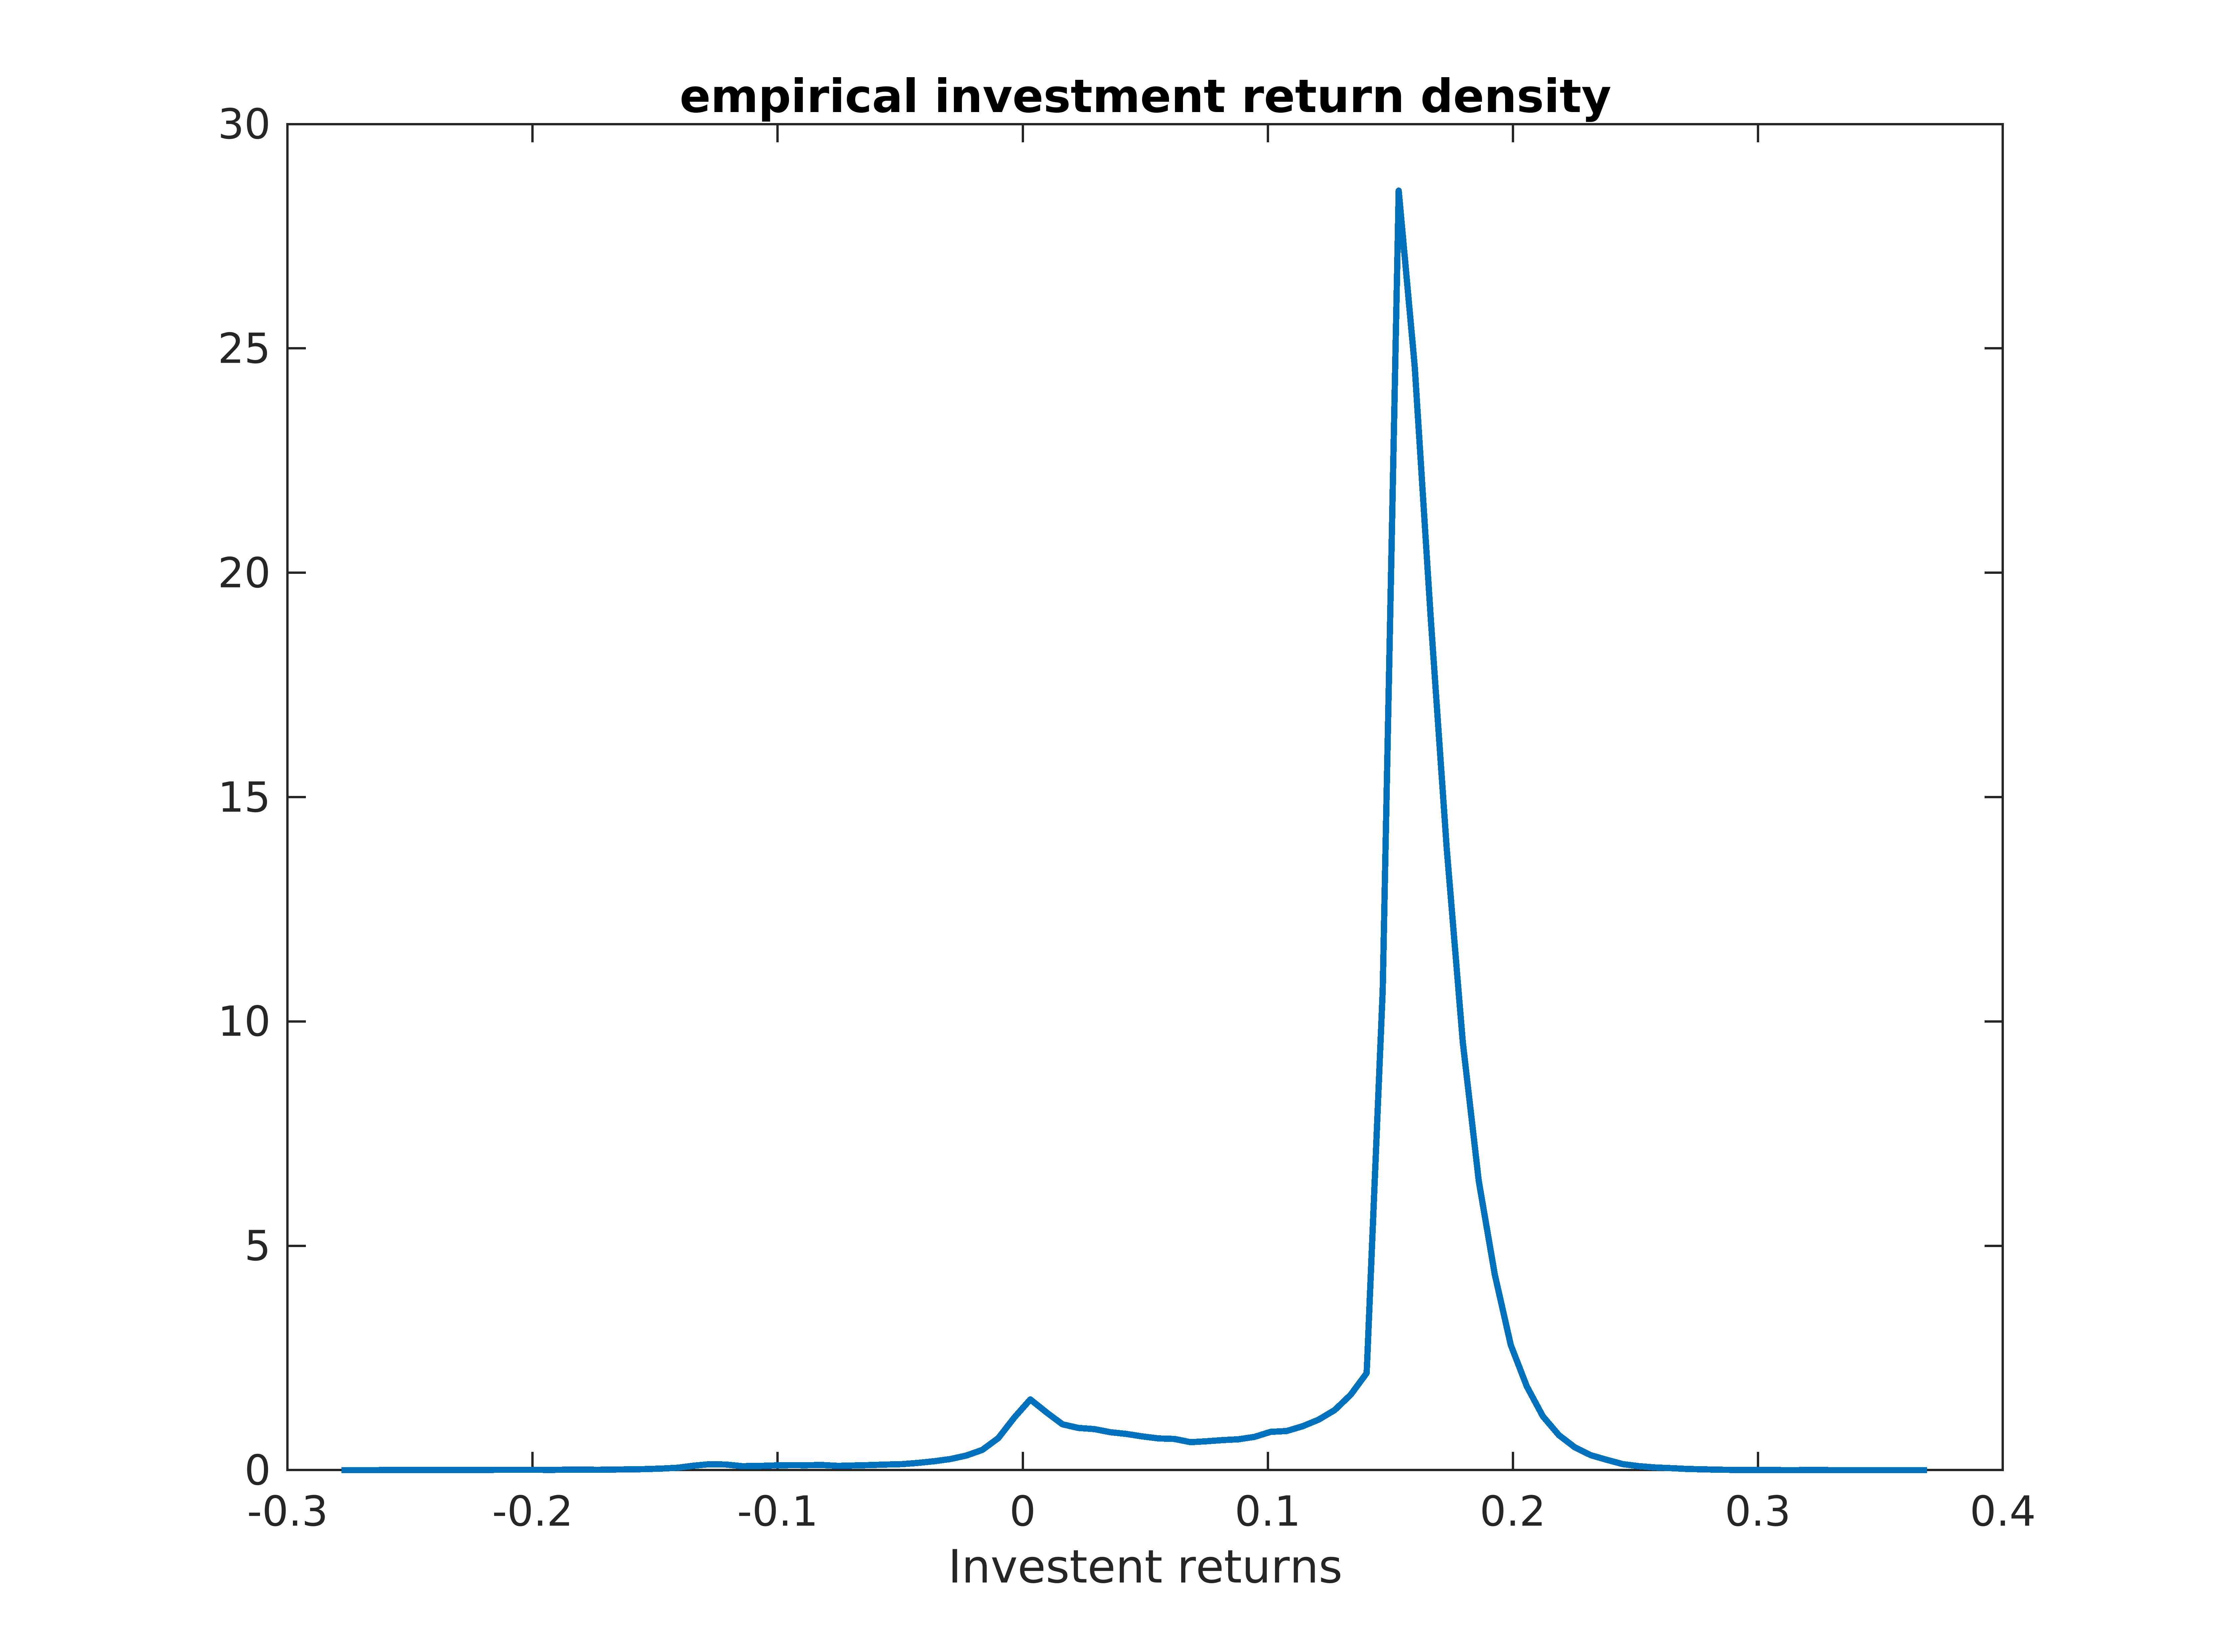
\includegraphics[scale = 0.4]{Images/Densityext1}
	\caption{Empirical density function of the annualized investment return when the risky asset is modeled as a \gls{GBM}.}
	\label{fig:ext1_investment_return}
\end{figure}
\begin{table}[]
	\centering
		\begin{tabular}{@{}lc@{}}
			\toprule
			Statistics & value  \\
			%\addlinespace[0.5em]
			\midrule
			$p^{\star}$ & 0.8834\\
			\addlinespace[0.5em]	
			$p_{MC}$ & 0.8835\\
			\addlinespace[0.5em]
			Mean Return (ann) & 5.40\%\\
			\addlinespace[0.5em]
			Volatility (ann) & 3.51\%\\
			\addlinespace[0.5em]
			Median Return (ann) & 5.94\%\\
			\addlinespace[0.5em]
			Skewness & -2.43\\
			\addlinespace[0.5em]
			Kurtosis & 12.30\\
			\addlinespace[0.5em]
			Sharpe Ratio & 1.249\\
			\addlinespace[0.5em]
			Avg horizon [years] & 3.70 \\
			\addlinespace[0.5em]
			yearly $V@R^{0.99}_{0.01}$ & 8.77\%\\	
			\bottomrule
		\end{tabular}
		\caption{Investment performance obtained via Monte-Carlo simulation with $2\times10^6$ replication at each rebalancing time.}
		\label{tab:performance_ext1}
\end{table}

\subsection{V@R constraint}
Although the probability of reaching the target set after 10 reallocations is quite high, Figure \ref{fig:ext1_investment_return} and the V@R figure in Table \ref{tab:performance_ext1} show that in some scenarios the loss could be particularly severe. We could hedge the portfolio against this downfall of performance by imposing an \textit{ex-ante} V@R constraint when synthesizing the allocation maps in the \gls{ODAA} algorithm, as we already did in the time-driven case and in Section \ref{subsec:Var_basic}. Once the investor has given us his risk profile through a monthly value-at-risk specification ($V@R^m_{1-\alpha}$), the idea is to bound portfolio volatility in the time span between two reallocations. In formula $\Var{w_{k+1}} \leq \sigma_{max}$, where $w_{k+1}$ is defined as follows
\begin{equation}\label{eq:return_ext1}
\frac{x_{k+1}-x_k}{x_k}\colon=w_{k+1}=\exp\{r\tau_{k+1}\}-1+u_k\widetilde{X}_{\tau_{k+1}}.
\end{equation}
and $\sigma_{max} = \frac{\sqrt{12\mathbb{E}[\tau_{k+1}]}V@R^m_{1-\alpha}}{z_{1-\alpha}}$.
We now want to compute the variance of random variable $w_{k+1}$. Using the fact that $\tau_{k+1} \perp \widetilde{X}_{\tau_{k+1}}$ (see \cite{baldi2017}), we have
\begin{equation}\label{eq:variance_ext1}
\Var{w_{k+1}} = \Var{\exp\{r\tau_{k+1}\}} + u_k^2\Var{\widetilde{X}_{\tau_{k+1}}}.
\end{equation}
Unfortunately, variance (\ref{eq:variance_ext1}) cannot be computed because $\exp\{r\tau_{k+1}\} \notin L^1(\Omega)$, which implies $\exp\{r\tau_{k+1}\} \notin L^2(\Omega)$. However, as the quantity $r\tau_{k+1}$ is small enough in our applications, we consider the first-order approximation of the exponential term in (\ref{eq:return_ext1}). In this way, portfolio variance becomes
\begin{equation}\label{eq:variance_ext1_approx}
\Var{w_{k+1}} = r^2\Var{\tau_{k+1}} + u_k^2\Var{\widetilde{X}_{\tau_{k+1}}}.
\end{equation}
The second term in (\ref{eq:variance_ext1_approx}) presents no particular difficulties, indeed we have $\Var{\widetilde{X}_{\tau_{k+1}}} = 4J^2p(1-p)$, where $p$ is given in Lemma \ref{lemma:probability_positive_jump}. More delicate is the computation of the first term. This means calculating $\mathbb{E}[\tau_{k+1}^2]$ and $\mathbb{E}[\tau_{k+1}]$.
In the following, we will give the detailed derivation of the first expectation, the second follows the same logic.


Using the well-known formula for the expectation of positive random variables together with the cdf (\ref{eq:cdf_ext1}), we obtain
\begin{align*}
\mathbb{E}[\tau_{k+1}^2] & = \int_{0}^{\infty}\mathbb{P}\big(\tau_{k+1}^2>t\big)\mathrm{d}t = \int_{0}^{\infty}\mathbb{P}\big(\tau_{k+1}>\sqrt{t}\big)\mathrm{d}t\\[1.5ex]
& = 2\cosh\Big(\frac{\widetilde{\mu}J}{\sigma^2}\Big)\int_{0}^{\infty}K_{\sqrt{t}}^{\infty}(J)\mathrm{d}t \\[1.5ex]
& = 2\cosh\Big(\frac{\widetilde{\mu}J}{\sigma^2}\Big)\frac{\sigma^2\pi}{4J^2}\sum_{n=1}^{\infty}\frac{n(-1)^{n+1}}{\alpha(n)}\sin(\frac{\pi}{2}n)
\underbrace{\int_{0}^{\infty}\exp\big\{-\alpha(n)\sqrt{t} \big\}\mathrm{d}t}_{2/\alpha(n)^2}\\
& = 2\cosh\Big(\frac{\widetilde{\mu}J}{\sigma^2}\Big)\frac{\sigma^2\pi}{4J^2}\sum_{n=1}^{\infty}\frac{2n(-1)^{n+1}}{\alpha(n)^3}\sin(\frac{\pi}{2}n)
\end{align*}
where we defined $\alpha(n) = \frac{\tilde{\mu}^2}{2\sigma^2} + \frac{\sigma^2n^2\pi^2}{8J^2}$. The expected interevent time is equal to

\begin{equation*}
\mathbb{E}[\tau_{k+1}] = 2\cosh\Big(\frac{\widetilde{\mu}J}{\sigma^2}\Big)\frac{\sigma^2\pi}{4J^2}\sum_{n=1}^{\infty}\frac{n(-1)^{n+1}}{\alpha(n)^2}\sin(\frac{\pi}{2}n).
\end{equation*}
The \textit{risk} constraint is now fully characterized, and therefore it can be used in the event-driven \gls{ODAA} algorithm to control the risky asset exposure. As a matter of fact, in order to implement it, we still need to address the issue related to the truncation of series $\sum_{n=1}^{\infty}\frac{n(-1)^{n+1}}{\alpha(n)^m}\sin(\frac{\pi}{2}n)$, where $m= 2,3$. The minimum number of terms $N$ required to obtained a residual smaller than $\epsilon$ could be derived as follows
\begin{align*}
\bigg\lvert \sum_{n=N+1}^{\infty}\frac{n(-1)^{n+1}}{\alpha(n)^m}\sin(\frac{\pi}{2}n)  \bigg\lvert   &\leq \sum_{n=N+1}^{\infty}\frac{n}{\alpha(n)^m}\\
& \leq \int_{N}^{\infty}\frac{n}{\big(\frac{\sigma^2n^2\pi^2}{8J^2}\big)^m}\mathrm{d}n\\
& = \Big(\frac{8J^2}{\sigma^2\pi^2}\Big)^m\frac{1}{(2m-2)}N^{-(2m-2)}\leq \epsilon
\end{align*}
which brings
\begin{equation}
N \geq \bigg\{\Big(\frac{8J^2}{\sigma^2\pi^2}\Big)^m\frac{1}{(2m-2)\epsilon}  \bigg\}^{\frac{1}{2m-2}}.
\end{equation}


The allocation maps obtained by adding the V@R constraint do not let the risky exposure exceed $68.41\%$.
In figure \ref{tab:performance_VaRext1} we report some sample statistics obtained by running a Monte Carlo simulation with $2\times10^6$ replications at each reallocation and the same investment parameters of the previous case. The \textit{ex-ante} monthly V@R specification has been set to $7\%$. 
\begin{table}[]
	\centering
	\begin{tabular}{@{}lc@{}}
		\toprule
		Statistics & value  \\
		%\addlinespace[0.5em]
		\midrule
		$p^{\star}$ & 0.7865\\
		\addlinespace[0.5em]	
		$p_{MC}$ & 0.7866\\
		\addlinespace[0.5em]
		Mean Return (ann) & 5.12\%\\
		\addlinespace[0.5em]
		Volatility (ann) & 3.18\%\\
		\addlinespace[0.5em]
		Median Return (ann) & 5.63\%\\
		\addlinespace[0.5em]
		Skewness & -1.62\\
		\addlinespace[0.5em]
		Kurtosis & 7.70\\
		\addlinespace[0.5em]
		Sharpe Ratio & 1.294\\
		\addlinespace[0.5em]
		Avg horizon [years] & 3.70 \\
		\addlinespace[0.5em]
		yearly $V@R^{0.99}_{0.01}$ & 6.10\%\\	
		\bottomrule
	\end{tabular}
	\caption{Investment performance obtained via Monte-Carlo simulation with $2\times10^6$ replication at each rebalancing time and the addition of the V@R constraint.}
	\label{tab:performance_VaRext1}
\end{table}


\section{Interest rate dynamics for the risk-free asset}\label{sec:Interest_rate_dynamics}
In this section we try to extend the model presented in Chapter \ref{chpt:ED} by assuming a dynamics for the interest rate of the bank account. Starting from the portfolio dynamics (\ref{eq:ptf_dynamic_ED}), our aim is replacing it with
\begin{equation}\label{eq:portfolio_dynamic_Vasicek}
\boxed{x_{k+1} = x_k\big( \exp\Big\{\int_{t_k}^{t_k+\tau_{k+1}}\!\!\!\!\!\!\!\!r_s\mathrm{d}s \Big\} + u_kJ\widetilde{N}_{k+1}\big)} \qquad k \in \mathbb{N}
\end{equation}
where $\{r_t\}_{t\geq t_k}$ is the short-rate process and everything else remains unchanged from Chapter \ref{chpt:ED}. Due to its analytical tractability, we decided to model the short-rate according to the Vasicek Model (see \cite{brigo2007}). The following \gls{SDE} provides the dynamics of the short-rate
\begin{equation}\label{eq:VasicekSDE}
\begin{cases*}
dr_t = a(b-r_t)dt + \sigma dW_t\\
r_{t_k} = r_k, \qquad t \geq t_k
\end{cases*}
\end{equation}
where $a,b,\sigma$ and $r_k$ are positive constant and $\{W_t\}_{t\geq t_k}$ an unidimensional Brownian motion. The main feature of the Vasicek model is the \textit{mean reversion} property: the process will tend to move to its average over time. Moreover, the process has a non-null probability to became negative. This is no longer a taboo since negative interest rates are seen in the market.

The solution of \gls{SDE} (\ref{eq:VasicekSDE}) is the following Ornstein–Uhlenbeck process
\begin{equation}\label{eq:solution_VasicekSDE}
r_t = r_ke^{-a(t-t_k)}+b(1-e^{-a(t-t_k)}) + \sigma e^{-a(t-t_k)}\int_{t_k}^{t}e^{a(s-t_k)}dW_s.
\end{equation}
However, we are interested in an explicit expression of the integrated version of process $r_t$ since it appears in the portfolio dynamics. For this reason, let us define the integrated short-rate process by $v_t=\int_{t_k}^{t}r_s\mathrm{d}s$. In order to find its explicit form, we integrate (\ref{eq:VasicekSDE}) from $t_k$ to a generic instant $t$, obtaining
\begin{equation}\label{eq:integrated_VasicekSDE}
r_t = r_k + a\big(b(t-t_k) - v_t\big) + \sigma(W_t-W_{t_k}).
\end{equation}
After equating (\ref{eq:integrated_VasicekSDE}) and (\ref{eq:solution_VasicekSDE}) and solving for $v_t$ we get
\begin{equation}\label{eq:v_t}
v_t = \frac{1}{a}\Big[(r_k-b)(1-e^{-a(t-t_k)})+ab(t-t_k)+\sigma\int_{t_k}^{t}(1-e^{-a(t-s)})dW_s\Big].
\end{equation}
From Appendix \ref{app:IntegratedOU} and (\cite{baldi2017}, Proposition 7.1) we have that
\begin{align}
\nonumber
v_t & \sim \mathcal{N}\Big(\eta(t-t_k),\zeta^2(t-t_k)\Big)\\[2ex]
\label{eq:Vasicek_mean}
\eta(t-t_k) & = \mathbb{E}[v_t]= \frac{1}{a}\Big[(r_k - b)\big(1-e^{-a(t-t_k)}\big)+ab(t-t_k)\Big]\\[2ex]
\label{eq:Vasicek_variance}
\zeta^2(t-t_k) & = \Var{v_t}= \frac{\sigma^2}{2a^3}\Big[2a(t-t_k) + 4e^{-a(t-t_k)}-e^{-2a(t-t_k)}-3\Big]
\end{align}
where $t \in \mathbb{R}^{+}$.
\begin{remark}
	The parameters $\eta(t-t_k)$ and $\zeta(t-t_k)$ depends only on the difference $t-t_k$, therefore the distribution of $v_t$ is stationary. This fact will be particularly useful in the following since the distribution of $v_{t_k+t}$ (which is the one we are interested in) depends only on $t$.
\end{remark}
\subsection{The density of $x_{k+1}$}
The last step is find the probability density function of the random variable $x_{k+1}$. 
\begin{proposition}
	Let $x_{k+1}$ be the random variable (\ref{eq:portfolio_dynamic_Vasicek}). Then, its probability density function is
	\begin{align*}
	f_{x_{k+1}}(z) &=\frac{p}{(z-\xi)}\bigg\{ \int_{0}^{\infty}\varphi\Big(\frac{\log\big(\frac{z-\xi}{x}\big)-\eta(t)}{\zeta(t)}\Big)\Big(\frac{1}{\zeta(t)}\Big)f_{\tau_{k+1}}(t)\mathrm{d}t\bigg\}\mathbbm{1}_{[x+\xi,\infty)} \nonumber +\\
	& + \frac{(1-p)}{(z+\xi)}\bigg\{ \int_{0}^{\infty}\varphi\Big(\frac{\log\big(\frac{z+\xi}{x}\big)-\eta(t)}{\zeta(t)}\Big)\Big(\frac{1}{\zeta(t)}\Big)f_{\tau_{k+1}}(t)\mathrm{d}t\bigg\}\mathbbm{1}_{[x-\xi,\infty)}
	\end{align*}
	where $\xi=xJu_k$, $f_{\tau_{k+1}}= \big\{\lambda e^{-\lambda t}\big\}\mathbbm{1}_{[0,\infty)}$ is the density of random variable $\tau_{k+1}$, $\varphi$ is the density of a standard normal and $\eta(t),\zeta(t)$ are functions (\ref{eq:Vasicek_mean}) and the square root of (\ref{eq:Vasicek_variance}) respectively computed in $t+t_k$.
\end{proposition}
\begin{proof}
	Let us rewrite the portfolio dynamics in the following way
	\[
	x_{k+1}=x\exp\{v_{t_k+\tau_{k+1}}\} + xJu_k\widetilde{N}_{k+1}=Y+\xi\widetilde{N}_{k+1}.
	\]
	The first step of the proof is finding the cdf of Y:
	\begin{align*}
	F_Y(y) & = \mathbb{P}\big(x\exp\{v_{t_k+\tau_{k+1}}\}\leq y\big)\\
	& = \int_{0}^{\infty}\mathbb{P}\Big(v_{t_k+\tau_{k+1}}\leq \log(y/x)\lvert \tau_{k+1}=t\Big)f_{\tau_{k+1}}(t)\mathrm{d}t\\
	& = \int_{0}^{\infty}\mathbb{P}\Big(v_{t_k+t}\leq \log(y/x)\Big)f_{\tau_{k+1}}(t)\mathrm{d}t\\
	& = \Bigg\{\int_{0}^{\infty}\varphi\Big(\frac{\log(y/x)-\eta(t)}{\zeta(t)}\Big)f_{\tau_{k+1}}(t)\mathrm{d}t \Bigg\}\mathbbm{1}_{[x,\infty)}
	\end{align*}
	where we used the Law of Total Probability in the continuous case and the fact that $v_{t_k+t}$ is Gaussian with parameters $\eta(t)$ and $\zeta(t)$ (which are the functions (\ref{eq:Vasicek_mean}) and the square root of (\ref{eq:Vasicek_variance}) respectively computed in $t+t_k$).
	
	
Repeating the usual steps, we are able to find the cdf of $x_{k+1}$:
\begin{align*}
F_{x_{k+1}}(z) & = \mathbb{P}\big(Y+\xi\widetilde{N}_{k+1}\big) \\
& = F_Y(z-\xi)p+F_Y(z+\xi)(1-p)\\
& = p\bigg\{ \int_{0}^{\infty}\Phi\Big(\frac{\log\big(\frac{z-\xi}{x}\big)-\eta(t)}{\zeta(t)}\Big)f_{\tau_{k+1}}(t)\mathrm{d}t\bigg\}\mathbbm{1}_{[x+\xi,\infty)}+\\
& + (1-p)\bigg\{ \int_{0}^{\infty}\Phi\Big(\frac{\log\big(\frac{z+\xi}{x}\big)-\eta(t)}{\zeta(t)}\Big)f_{\tau_{k+1}}(t)\mathrm{d}t\bigg\}\mathbbm{1}_{[x-\xi,\infty)}.
\end{align*}
where $\Phi$ is the cdf of a standard normal and $p$ the probability that $\widetilde{N}_{k+1}$ is equal to 1. Finally, deriving with respect to $z$ under the integral sign gives us the result.
\end{proof}
\subsection{The calibration of the Vasicek model}
In this section we see how parameters $a$, $b$ and $\sigma$ of the Vasicek model can be calibrated to data using the linear regression. We closely follow \cite{Bernal2016}.

The first step is to discretize Equation (\ref{eq:VasicekSDE}) in order to find a linear relation 
\begin{align}\label{eq:Vasicek_discretized}
\nonumber
r_{t+\Delta t} & = r_t + a(b-r_t)\Delta t+\sigma\sqrt{\Delta t}Z \\
& = (1-a\Delta t)r_t+ab\Delta t+\sigma\sqrt{\Delta t}Z
\end{align}
where $Z \sim \mathcal{N}(0,1)$. From (\ref{eq:Vasicek_discretized}) is clear the linear relation between $r_{t+\Delta t}$ and $r_t$. Therefore, the above equation can be rewritten in a fashion suitable for the linear regression estimation as follows
\[
r_{t+\Delta t} = \alpha r_t + \beta + \varepsilon
\]
where 
\begin{equation*}
\begin{cases*}
\alpha = 1-a\Delta t\\
\beta = ab\Delta t
\end{cases*}
\end{equation*}
and $\varepsilon \sim \mathcal{N}(0,\sigma^2\Delta t)$ is the error term. Let us suppose to have a random sample $\{r_1,\ldots,r_n\}$ (for example daily 3-month LIBOR). The independent variable and the response are
\[ \bm{y} = \begin{bmatrix}
r_2\\
\vdots\\
r_n
\end{bmatrix} \qquad
\bm{x}= \begin{bmatrix}
r_1\\
\vdots\\
r_{n-1}
\end{bmatrix}.
\]
The linear relation between $\bm{y}$ and $\bm{x}$ is reported in Figure (\ref{fig:linear_regression}).

\begin{figure}
	\centering
	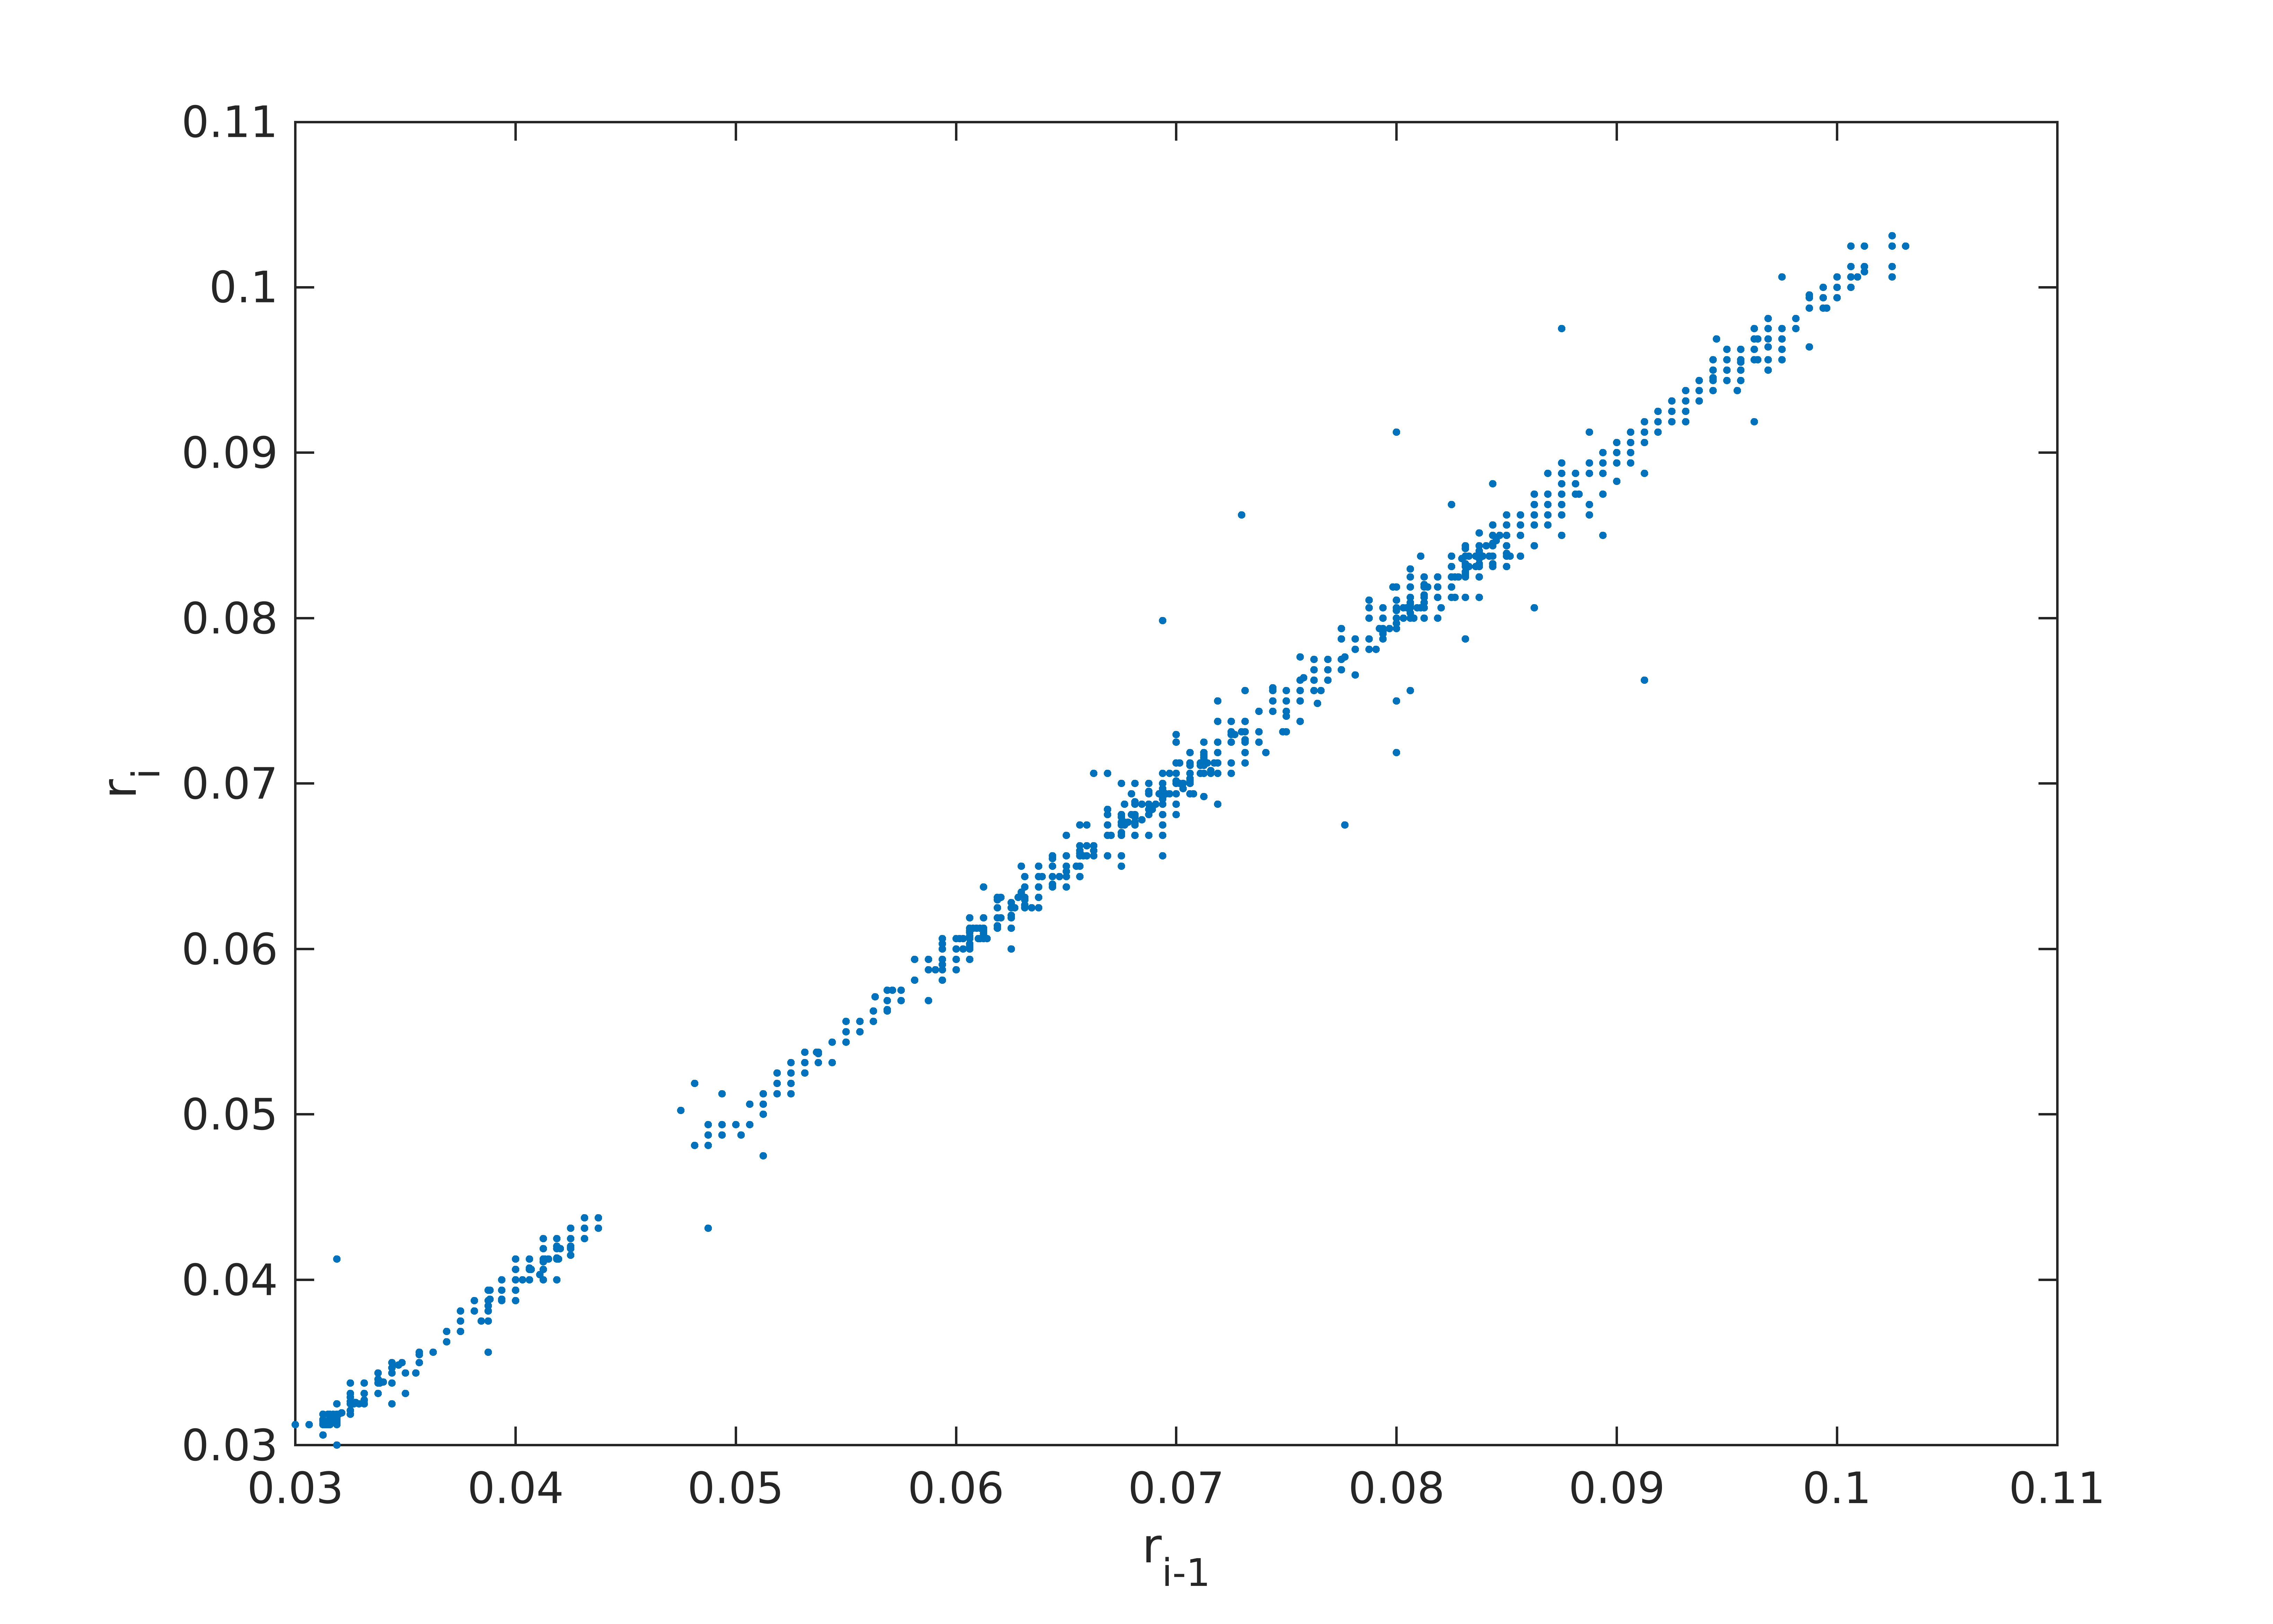
\includegraphics[scale=0.5]{Images/LinearRegression}
	\caption{linear relation between consecutive daily 3-month LIBOR rate quotes. }
	\label{fig:linear_regression}
\end{figure}


Once the least square estimates $\widehat{\alpha}$ and $\widehat{\beta}$ have been found, we can recover the estimates of the Vasicek model parameters in the following way
\begin{equation*}
\begin{cases*}
\widehat{a}=\frac{1}{\Delta t}(1-\widehat{\alpha})\\[2ex]
\widehat{b}= \widehat{\beta}/(\widehat{a}\Delta t)\\[2ex]
\widehat{\sigma}=\frac{RSE}{\Delta t}
\end{cases*}
\end{equation*}
where $RSE$ is the residual standard error of the fitting.

Applying this method to daily ($\Delta t = 1/252$) quotes of 3-month LIBOR starting from 22 January 2010 to 25 April 2016 brings the following estimates
\begin{equation*}
\begin{cases*}
\widehat{a}=0.1670\\
\widehat{b}=0.0280 \\
\widehat{\sigma}=0.0160
\end{cases*}.
\end{equation*}














\subsection{Numerical results}





\chapter{Conclusions}\label{chpt:Conclusions}
In this final chapter we summarize what has been achieved in this thesis and then suggest some directions for future research.

\section{The thesis in a nutshell}
Recent results in Stochastic Reachability have been the basis for this thesis. These results (e.g. the \gls{ODAA} theorem) allowed us to cast the asset allocation problem in a Control System setting. The generality of this approach permitted portfolio rebalancings to be driven first by time and then by the occurrence of discrete events. In the time-driven case, a universe of three asset classes (Cash, Bond and Equity) was considered and the allocation maps for a 2-year investment were obtained. These maps exhibited a \textit{contrarian} attitude: the higher the portfolio performance the less risky the asset class mix, the lower the performance the riskier the mix. In the 2-year investment example, the \gls{ODAA} strategy outperformed both the \gls{CPPI} and the constant-mix in terms of annualized returns while showing a comparable risk profile. In the event-driven case, the portfolio consisted of a risk-free asset (a bank account) and a risky asset (an exposure to a future index). In this context, the risky asset allocation maps, obtained via \gls{ODAA} algorithm, showed a \textit{contrarian} behavior in the sense that when portfolio performance is up the risky asset is shorted, when it is down a long position is taken instead.

As far as the time-driven model is concerned, a small contribution to the literature has been the use of Generalized Hyperbolic distributions, as an alternative to the Gaussian Mixture model proposed in \cite{Pola12}, to describe the statistical properties of asset class returns.
The personal contribution to the event-driven literature has been the extension of the model introduced in \cite{specchio2011} in two innovative ways. In particular, first the risky asset has been modeled as a Geometric Brownian Motion, then an interest rate dynamics as been considered for the bank account. In the first case, the usual \textit{contrarian} allocation maps for the risky asset were obtained. In the second case, the complexity of the formulas involved made the implementation quite difficult; a future research direction could be finding suitable numerical methods to tackle these issues. 
\section{Further developments}
The first idea could be casting the asset allocation problem in a stochastic hybrid system setting. A stochastic hybrid system is a control system whose evolution has a continuous and a discrete component. For instance, the problem of maintaining the temperature of $r \in \mathbb{N}$ different rooms within a certain range over time could be modeled as a stochastic hybrid system. The discrete state space being the mode (ON or OFF) of the heater switches and the continuous state space the room temperatures. In an asset allocation problem, the discrete state space could be the states of the economy. Main references are \cite{ABATE2008} for the discrete-time case and \cite{Boj2012} for the continuous-time case.






%----------------------------------------------------------------------------------------
%	THESIS CONTENT - APPENDICES
%----------------------------------------------------------------------------------------

\appendix
\chapter{Probability Distributions} \label{app:B}
In this appendix we give further details about the probability distributions used in part I. Main references are \cite{Brey2013}, \cite{paolella2007intermediate} and \cite{McNeil2005}.
\section{Generalized Inverse Gaussian}
\begin{definition}[Bessel function]
	The modified Bessel function of the third kind (simply called \textbf{Bessel function}) is defined as \[ K_{\nu}(x) = \frac{1}{2}\int_{0}^{\infty}t^{\nu-1}\exp\big\{-\frac{1}{2}x(t + t^{-1})\big\}\mathrm{d}t, \quad x > 0.  \]
\end{definition}
\begin{definition}[Generalized Inverse Gaussian]
	the density of a \textbf{Generalized Inverse Gaussian} (GIG) random variable $W$ $(W \sim \mathcal{N}^-\big(\lambda,\chi,\psi \big))$ is 
	\begin{equation}\label{eq:GIGdensity}
	f_{GIG}(w) = \Big(\frac{\psi}{\chi}\Big)^{\frac{\lambda}{2}}\frac{w^{\lambda-1}}{2K_{\lambda}(\sqrt{\chi\psi})}\exp\Big\{-\frac{1}{2}\big(\frac{\chi}{w}+\psi w\big)\big)\Big\} 
	\end{equation}
	with parameters satisfying 
	\[
	\begin{cases}
	\chi >0,\psi \geq 0, \quad \text{if} \quad \lambda <0\\
	\chi >0,\psi > 0, \quad \text{if} \quad \lambda =0\\
	\chi \geq0,\psi > 0, \quad \text{if} \quad \lambda >0\\
	\end{cases}
	\]
\end{definition}
\paragraph{Useful formulas}
The following formulas are used in the text:
\begin{equation}\label{eq:GIG_moment}
\mathbb{E}[W^n] = \Big(\frac{\chi}{\psi}\Big)^{\frac{n}{2}}\frac{K_{\lambda+n}(\sqrt{\chi\psi})}{K_{\lambda}(\sqrt{\chi\psi})}
\end{equation}
\begin{equation}\label{eq:GIG_log}
\mathbb{E}[\log W] = \Big\{\frac{\mathrm{d}\mathbb{E}[X^{\alpha}]}{\mathrm{d}\alpha}\Big\}_{\alpha=0}
\end{equation}
\section{Density Functions}
We give here the probability density function for the general multivariate GH distribution and same special cases
\subsection{GH}
\begin{equation}
f(\bm{x}) = c\frac{K_{\lambda-\frac{m}{2}}\Big(\sqrt{\big(\chi+Q(\bm{x})\big)\big(\psi+\bm{\gamma}^T\bm{\Sigma}^{-1}\bm{\gamma} \big)}\Big)\exp\big\{(\bm{x}-\bm{\mu})^T\Sigma^{-1}\bm{\gamma}\big\}}{\Big(\sqrt{\big(\chi+Q(\bm{x})\big)\big(\psi+\bm{\gamma}^T\bm{\Sigma}^{-1}\bm{\gamma} \big)}\Big)^{\frac{m}{2}-\lambda}}
\end{equation}
where $Q(\bm{x})=(\bm{x}-\bm{\mu})^T\bm{\Sigma}^{-1}(\bm{x}-\bm{\mu})$ and \[ c=\frac{\big(\sqrt{\chi\psi}\big)^{-\lambda}\psi^{\lambda}\big(\psi+\bm{\gamma}^T\bm{\Sigma}^{-1}\bm{\gamma} \big)^{\frac{m}{2}-\lambda}}{(2\pi)^{\frac{m}{2}}\lvert\bm{\Sigma}\lvert^{\frac{1}{2}}K_{\lambda}(\sqrt{\chi\psi})}  \]
\subsection{Student-t}
Setting the degree of freedom $\nu=-2\lambda$ the density reads
\begin{equation}
f(\bm{x}) = c\frac{K_{\frac{\nu+m}{2}}\Big(\sqrt{\big(\nu-2+Q(\bm{x})\big)\big(\bm{\gamma}^T\bm{\Sigma}^{-1}\bm{\gamma}\big)}\Big)\exp\big\{(\bm{x}-\bm{\mu})^T\Sigma^{-1}\bm{\gamma}\big\}}{\Big(\sqrt{\big(\nu-2+Q(\bm{x})\big)\big(\bm{\gamma}^T\bm{\Sigma}^{-1}\bm{\gamma}\big)}\Big)^{\frac{\nu+m}{2}}}
\end{equation}
where \[ c = \frac{\big(\nu-2\big)^{\frac{\nu}{2}}\big(\bm{\gamma}^T\bm{\Sigma}^{-1}\bm{\gamma}\big)^{\frac{\nu+m}{2}}}{(2\pi)^{\frac{m}{2}}\lvert\bm{\Sigma}\lvert^{\frac{1}{2}}\Gamma(\frac{\nu}{2})2^{\frac{\nu}{2}-1}} \]
\subsection{VG}
\begin{equation}
f(\bm{x}) = c\frac{K_{\lambda-\frac{m}{2}}\Big(\sqrt{Q(\bm{x})\big(2\lambda+\bm{\gamma}^T\bm{\Sigma}^{-1}\bm{\gamma} \big)}\Big)\exp\big\{(\bm{x}-\bm{\mu})^T\Sigma^{-1}\bm{\gamma}\big\}}{\Big(\sqrt{Q(\bm{x})\big(2\lambda+\bm{\gamma}^T\bm{\Sigma}^{-1}\bm{\gamma} \big)}\Big)^{\frac{m}{2}-\lambda}}
\end{equation}
where \[ c=\frac{2\lambda^{\lambda}\big(2\lambda+\bm{\gamma}^T\bm{\Sigma}^{-1}\bm{\gamma}\big)^{\frac{m}{2}-\lambda}}{(2\pi)^{\frac{m}{2}}\lvert\bm{\Sigma}\lvert^{\frac{1}{2}}\Gamma(\lambda)} \]





\input{Appendix/AppendixC}


\backmatter
%----------------------------------------------------------------------------------------
%	BIBLIOGRAPHY
%----------------------------------------------------------------------------------------

\backmatter
\nocite{*}
\bibliographystyle{acm}
\bibliography{Bibliography/biblio}



\end{document}          
